%\graphicspath{{./Imagenes/03/}}
\chapter{Resultados Obtenidos y Análisis}

\section{Pruebas unidimensionales}

\subsection{Test 1}
Sea $u=u(x)$ la función incognita, se resuelve la siguiente ecuacion dada por:
\begin{equation}
    -\frac{d^2u}{dx^2} + \frac{du}{dx} + u = f
\end{equation}
donde $f= (1+4\pi^2) \sin(2\pi x) - 2\pi\cos(2\pi x)$, para $x \in [0,1]$ sometido a condiciones de dirichlet homogeneas:
\begin{equation}
 u|_{x=0} = 0 \; , \; u|_{x=1}=0
\end{equation}
La solución exacta al problema es:
\begin{eqnarray}
    u = \sin( 2 \pi x ) \\
    \frac{du}{dx} = 2 \pi \cos( 2 \pi x )
\end{eqnarray}
Por fines investigativos, se resulve el mismo problema imponiendo condiciones naturales, es decir, considerando condiciones de Dirichlet - Neumann y Neumann - Dirichlet en los extremos izquierdo y derecho respectivamente. En la Figura \ref{fig:T1_caso-1_sol} se muestra la solución dada para 21 puntos de colocación utilizando la función de forma Maxent. En las Figuras \ref{fig:T1_caso-1_conv} \ref{fig:T1_caso-2_conv} y \ref{fig:T1_caso-3_conv} se muestras la convergencia de la solución
\begin{figure}
    \centering
    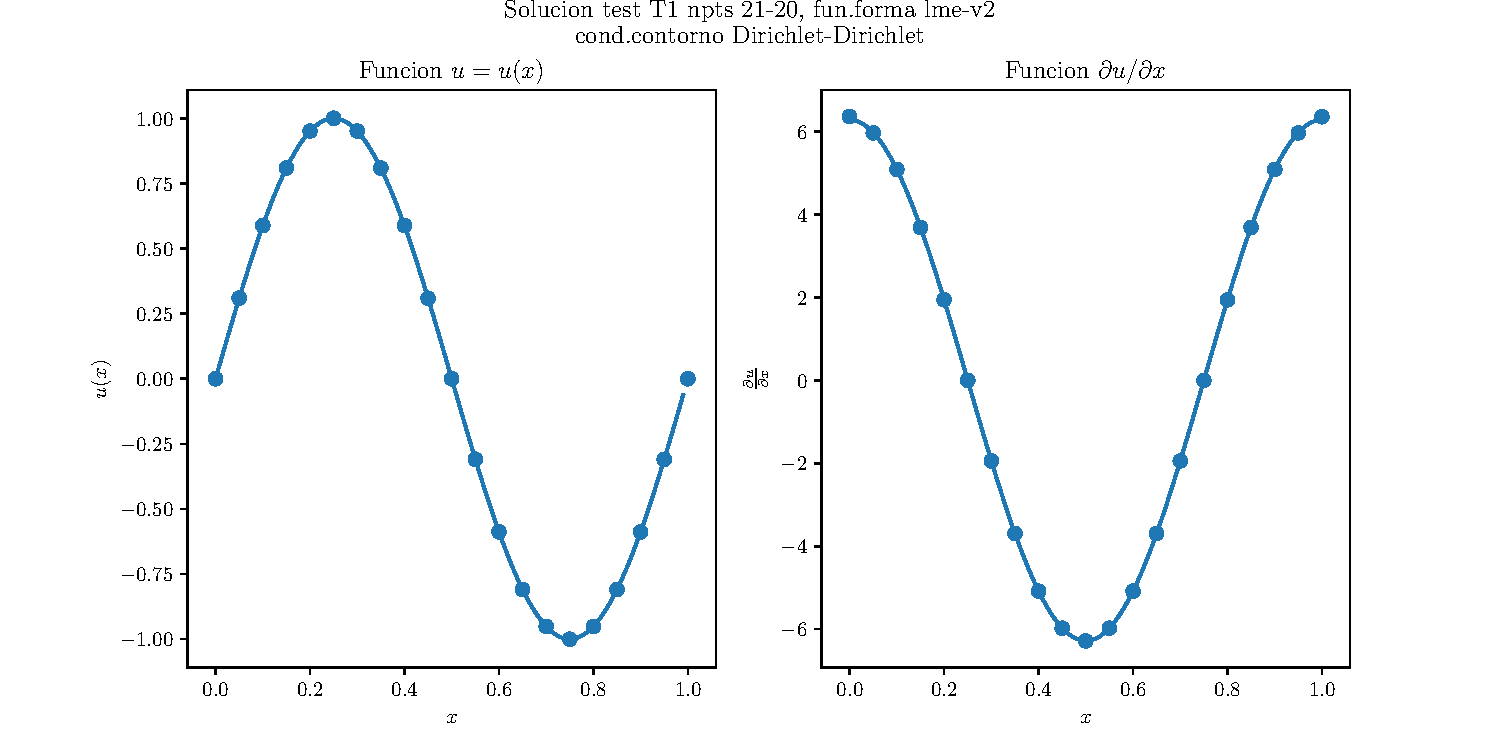
\includegraphics[width=1\textwidth]{./Imagenes/06/solucion/T1_21-20_regular_type-2_caso-1_lme-v2_direct_dgesv-lapack-blas.pdf}
    \caption{Solución del test T1} \label{fig:T1_caso-1_sol}
\end{figure}
%%%%%%%%%%%%%%%%%%%%%%%%%%%%%%%%%%%%%%%%%
\begin{figure}
    \centering
    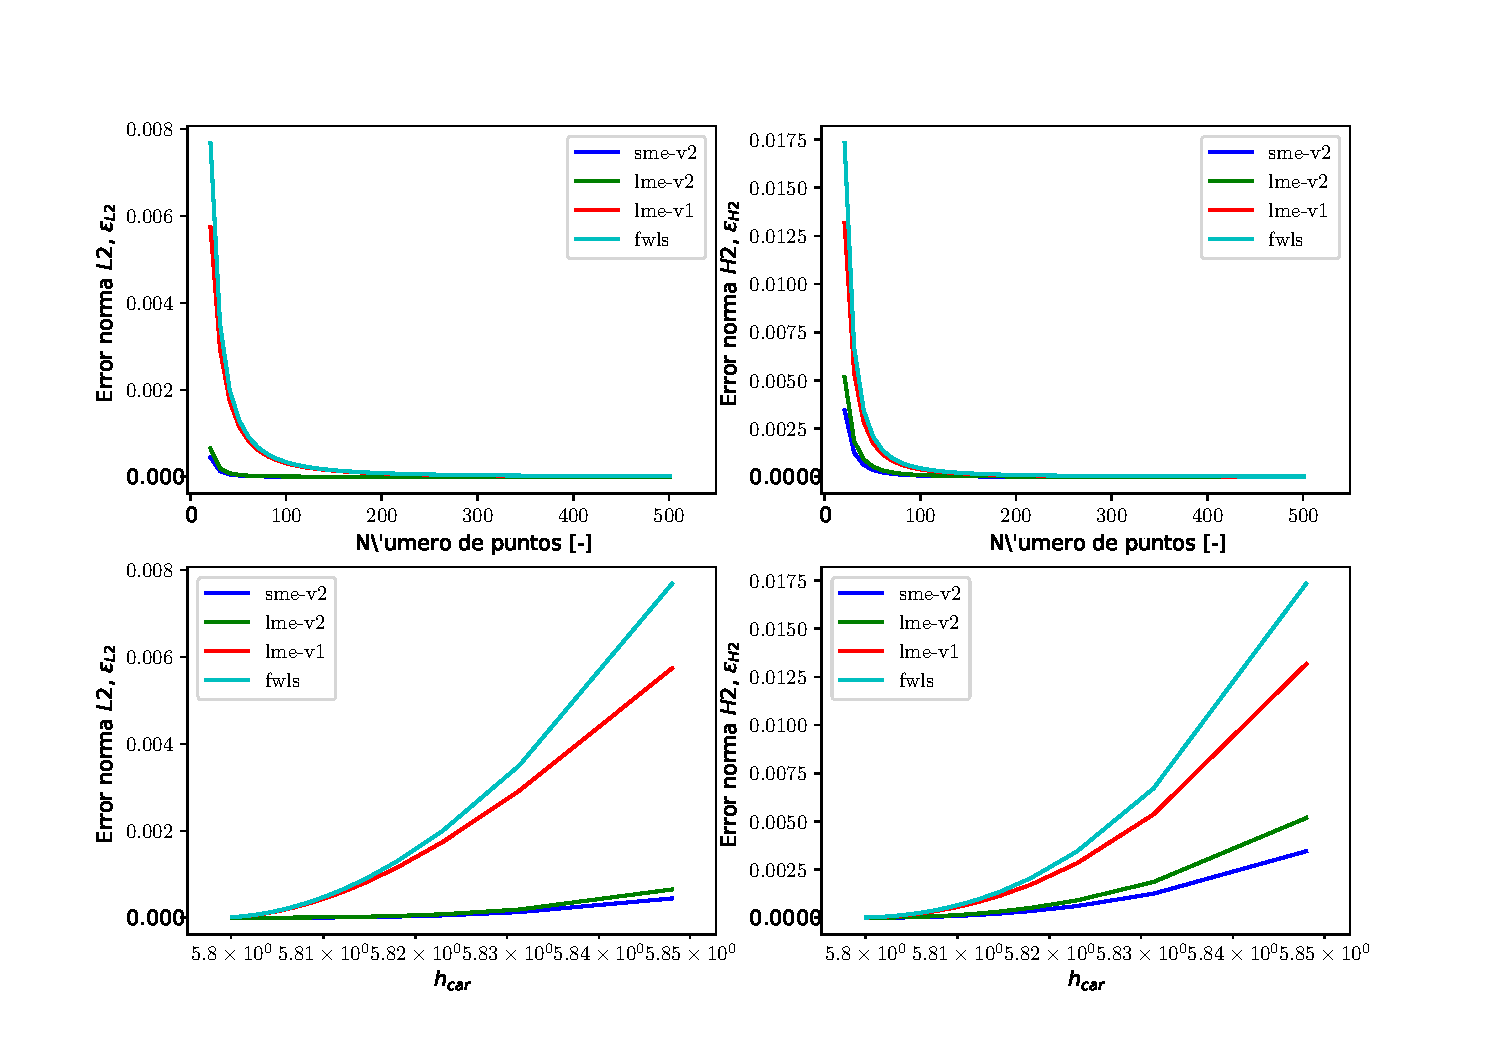
\includegraphics[width=1\textwidth]{./Imagenes/06/comparacion_shp_regular/T1_regular_type-2_caso-1_direct_dgesv-lapack-blas_sme-v2_lme-v2_lme-v1_fwls.pdf}
    \caption{Convergencia test T1 sujeto a condiciones Dirichlet - Dirichlet para una distribución regular} \label{fig:T1_caso-1_conv}
\end{figure}
\begin{figure}
    \centering
    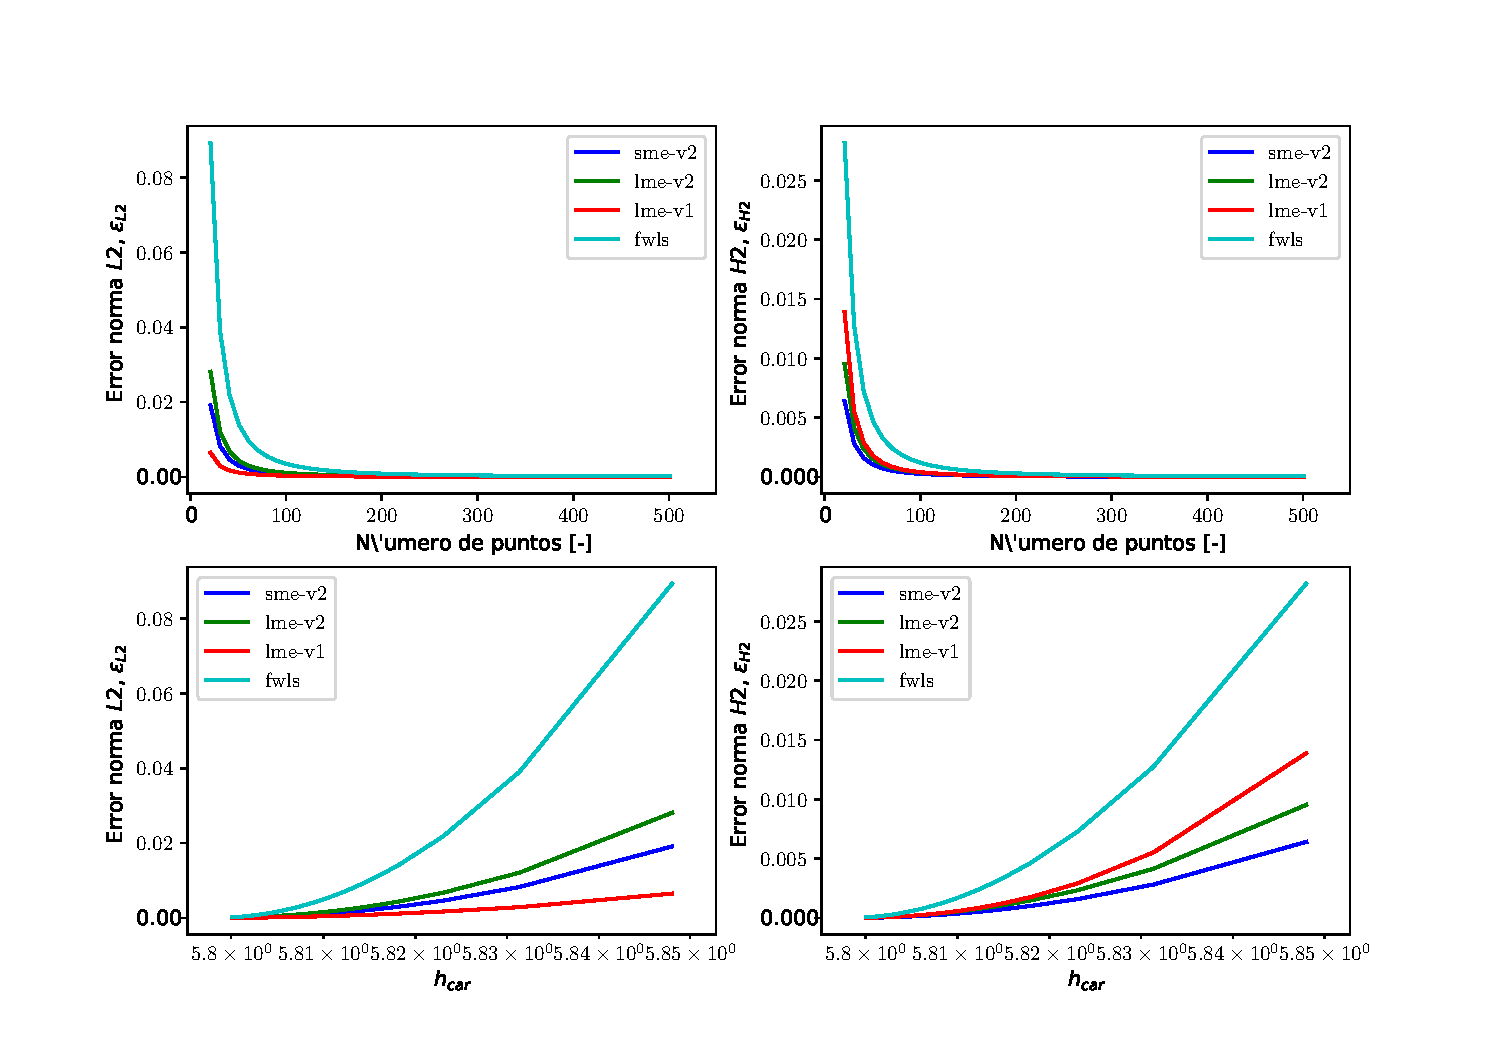
\includegraphics[width=1\textwidth]{./Imagenes/06/comparacion_shp_regular/T1_regular_type-2_caso-2_direct_dgesv-lapack-blas_sme-v2_lme-v2_lme-v1_fwls.pdf}
    \caption{Convergencia test T1 sujeto a condiciones Dirichlet - Neumann para una distribución regular} \label{fig:T1_caso-2_conv}
\end{figure}
\begin{figure}
    \centering
    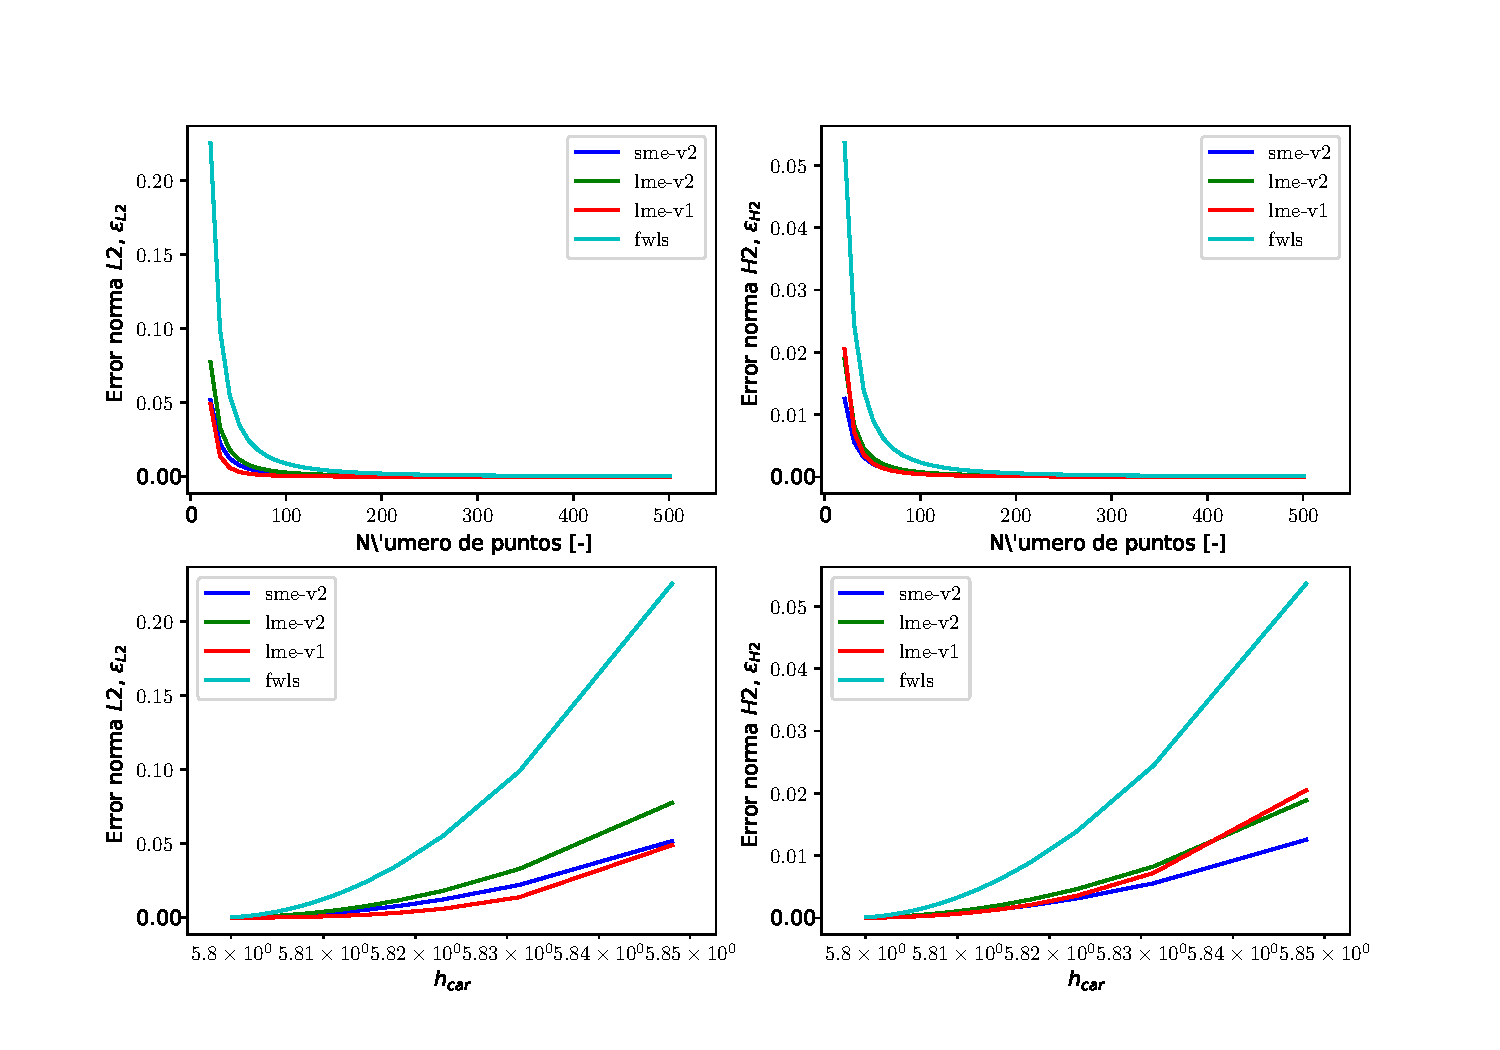
\includegraphics[width=1\textwidth]{./Imagenes/06/comparacion_shp_regular/T1_regular_type-2_caso-3_direct_dgesv-lapack-blas_sme-v2_lme-v2_lme-v1_fwls.pdf}
    \caption{Convergencia test T1 sujeto a condiciones Neumann - Dirichlet para una distribución regular} \label{fig:T1_caso-3_conv}
\end{figure}
%%%%%%%%%%%%%%%%%%%%%%%%%%%%%%%%%%%%%%%%%
\begin{figure}
    \centering
    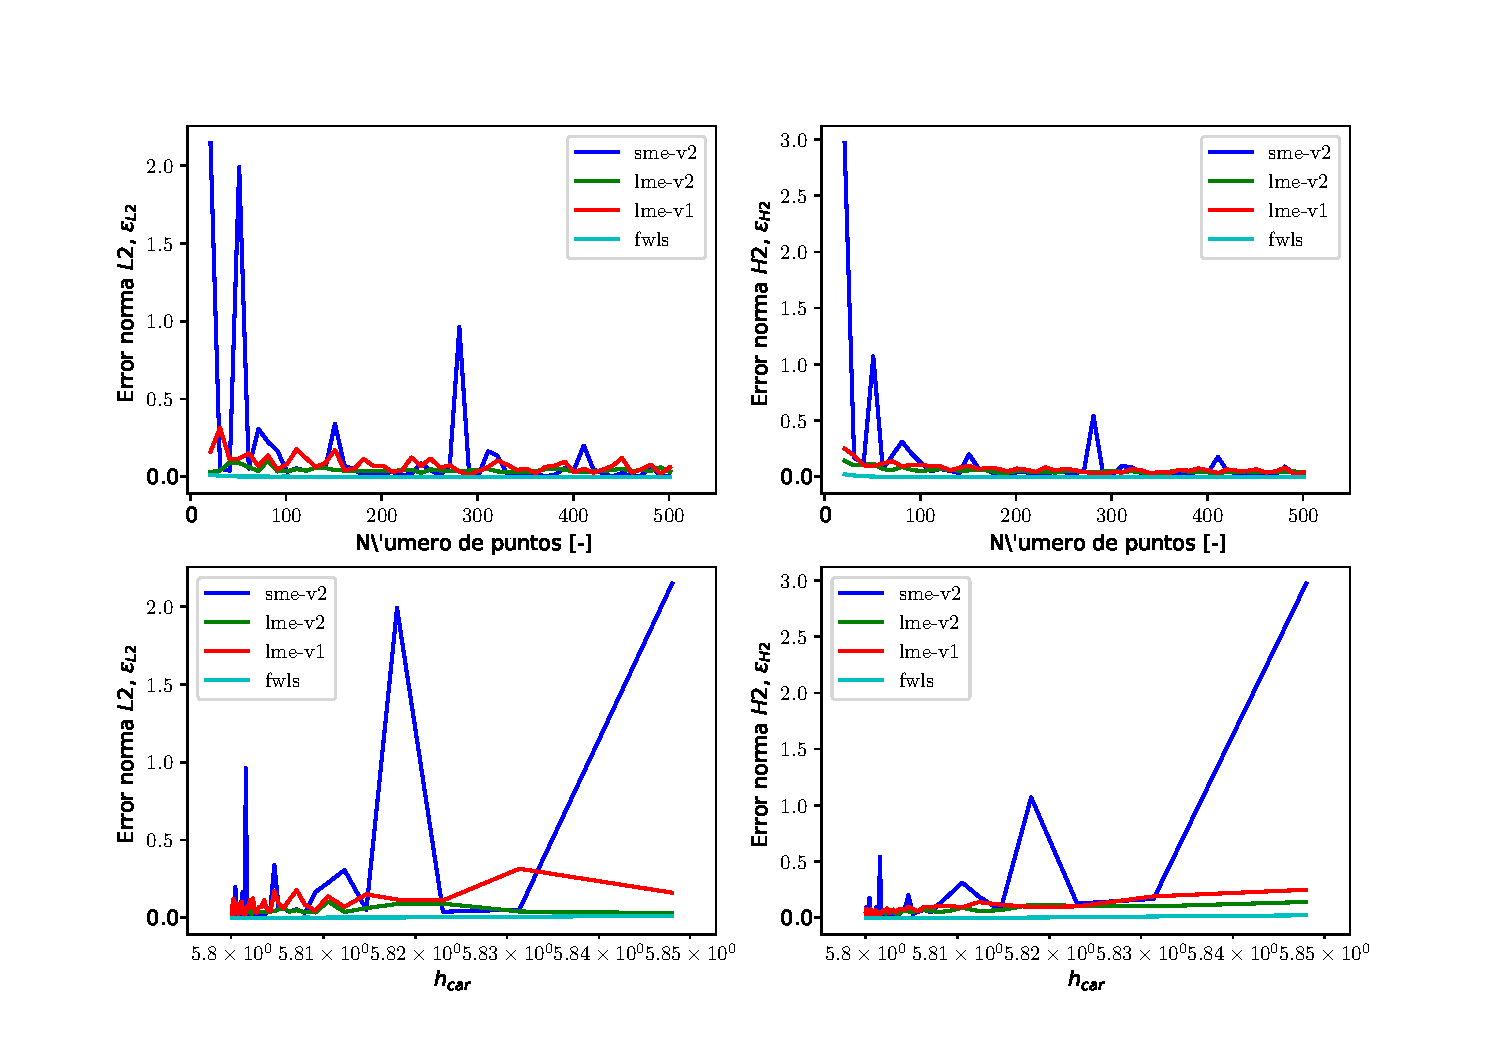
\includegraphics[width=1\textwidth]{./Imagenes/06/comparacion_shp_irreg/T1_irreg_type-2_caso-1_direct_dgesv-lapack-blas_sme-v2_lme-v2_lme-v1_fwls.pdf}
    \caption{Convergencia test T1 sujeto a condiciones Dirichlet - Dirichlet para una distribución irregular} \label{fig:T1_caso-1_conv_irreg}
\end{figure}
\begin{figure}
    \centering
    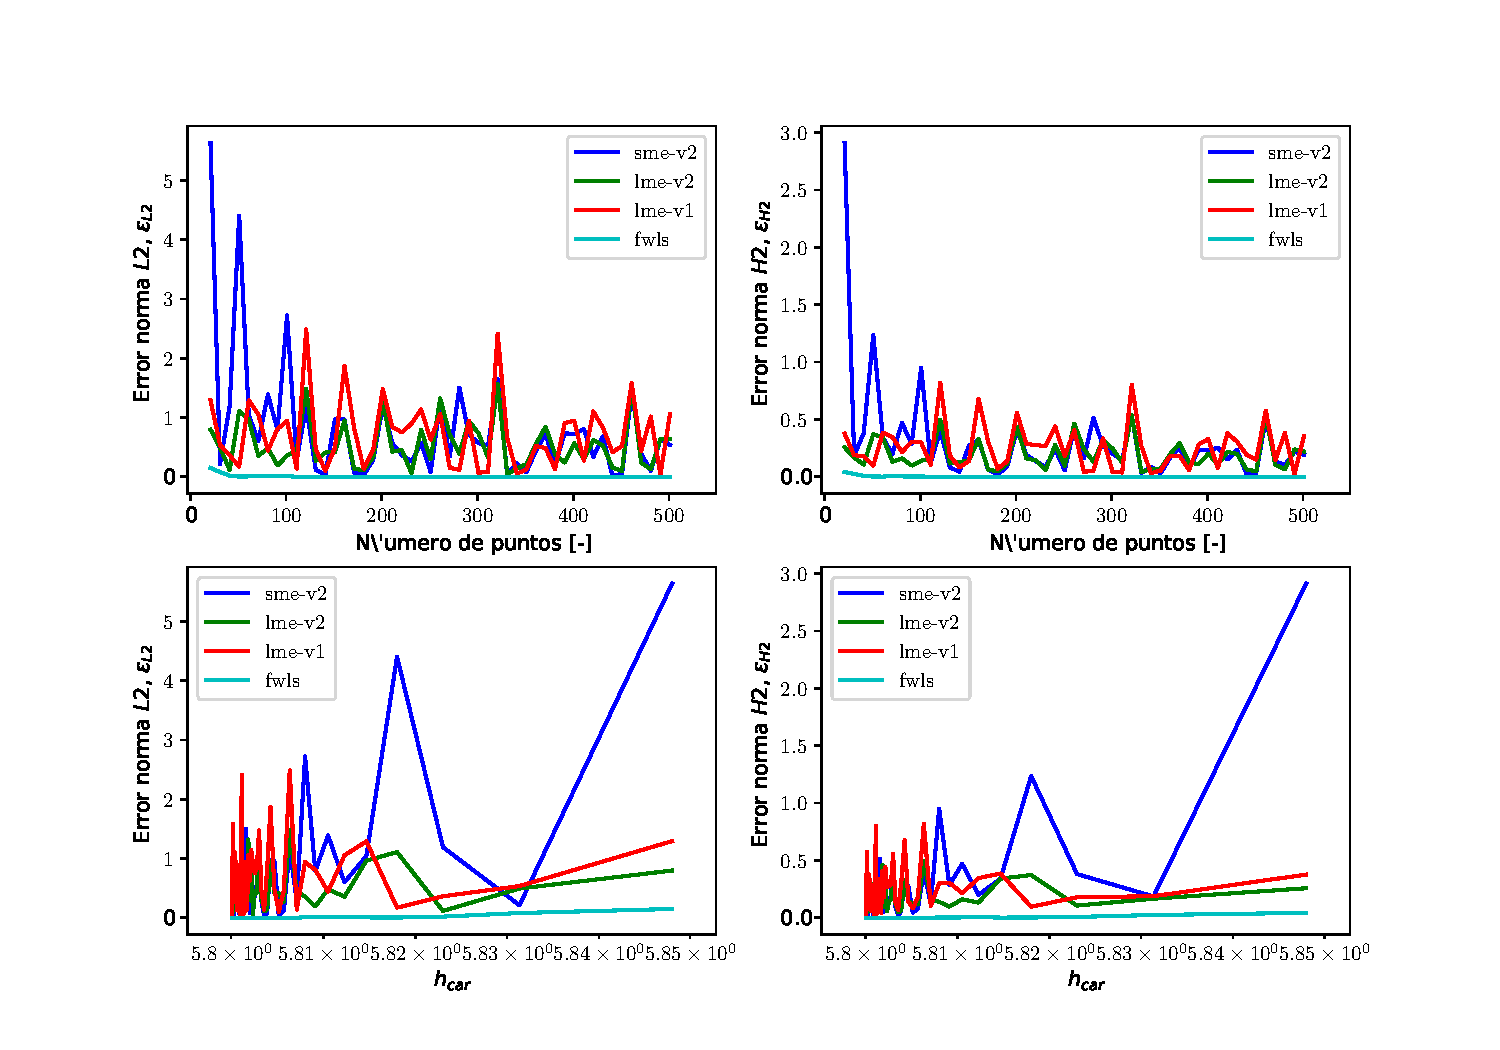
\includegraphics[width=1\textwidth]{./Imagenes/06/comparacion_shp_irreg/T1_irreg_type-2_caso-2_direct_dgesv-lapack-blas_sme-v2_lme-v2_lme-v1_fwls.pdf}
    \caption{Convergencia test T1 sujeto a condiciones Dirichlet - Neumann para una distribución irregular} \label{fig:T1_caso-2_conv_irreg}
\end{figure}
\begin{figure}
    \centering
    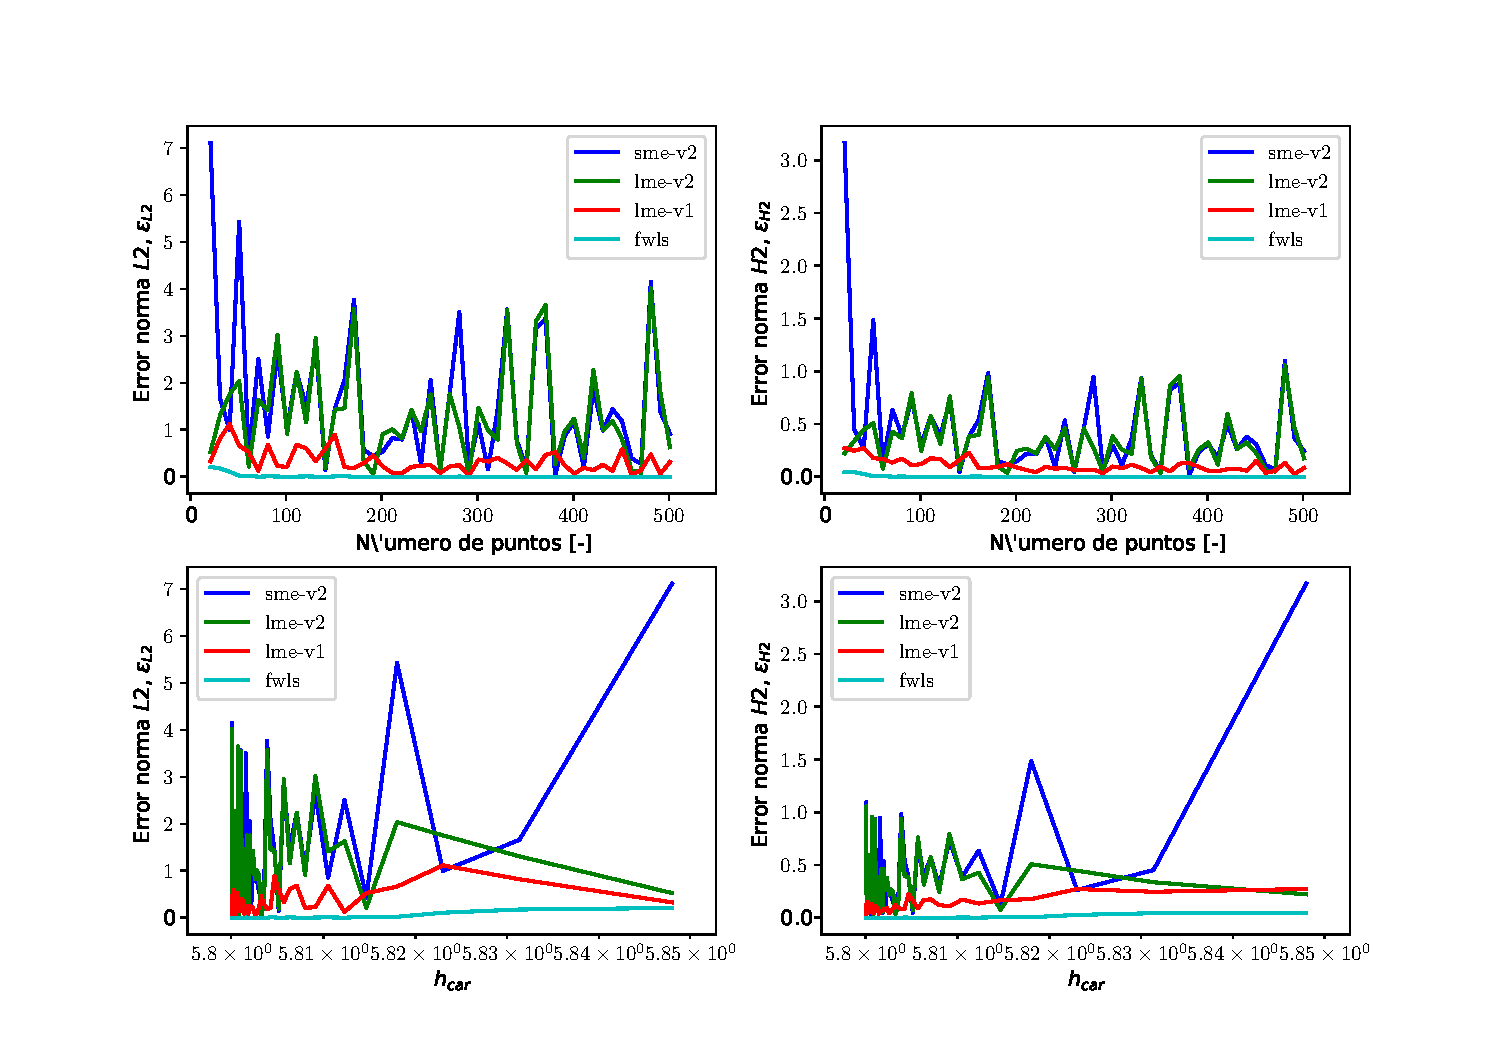
\includegraphics[width=1\textwidth]{./Imagenes/06/comparacion_shp_irreg/T1_irreg_type-2_caso-3_direct_dgesv-lapack-blas_sme-v2_lme-v2_lme-v1_fwls.pdf}
    \caption{Convergencia test T1 sujeto a condiciones Neumann - Dirichlet para una distribución irregular} \label{fig:T1_caso-3_conv_irreg}
\end{figure}


\subsection{Test 2}
Se resuelve la siguiente ecuación:
\begin{equation}
    u = 1 - x^3 + exp( -100x^2 )
\end{equation}
cuya solución exacta es
\begin{eqnarray}
    u  = 1 - x^3 + exp(-100 x^2 )
    du = - 3 x^2 -200 x \exp(-100 x^2 )
\end{eqnarray}
En la Figura \ref{fig:T2_caso-1_sol} aparece la gráfica de la solución aproximada, y en las Figuras \ref{fig:T2_caso-1_conv} \ref{fig:T2_caso-2_conv} y \ref{fig:T2_caso-3_conv} se muestra la convergencia de la solución
\begin{figure}
    \centering
    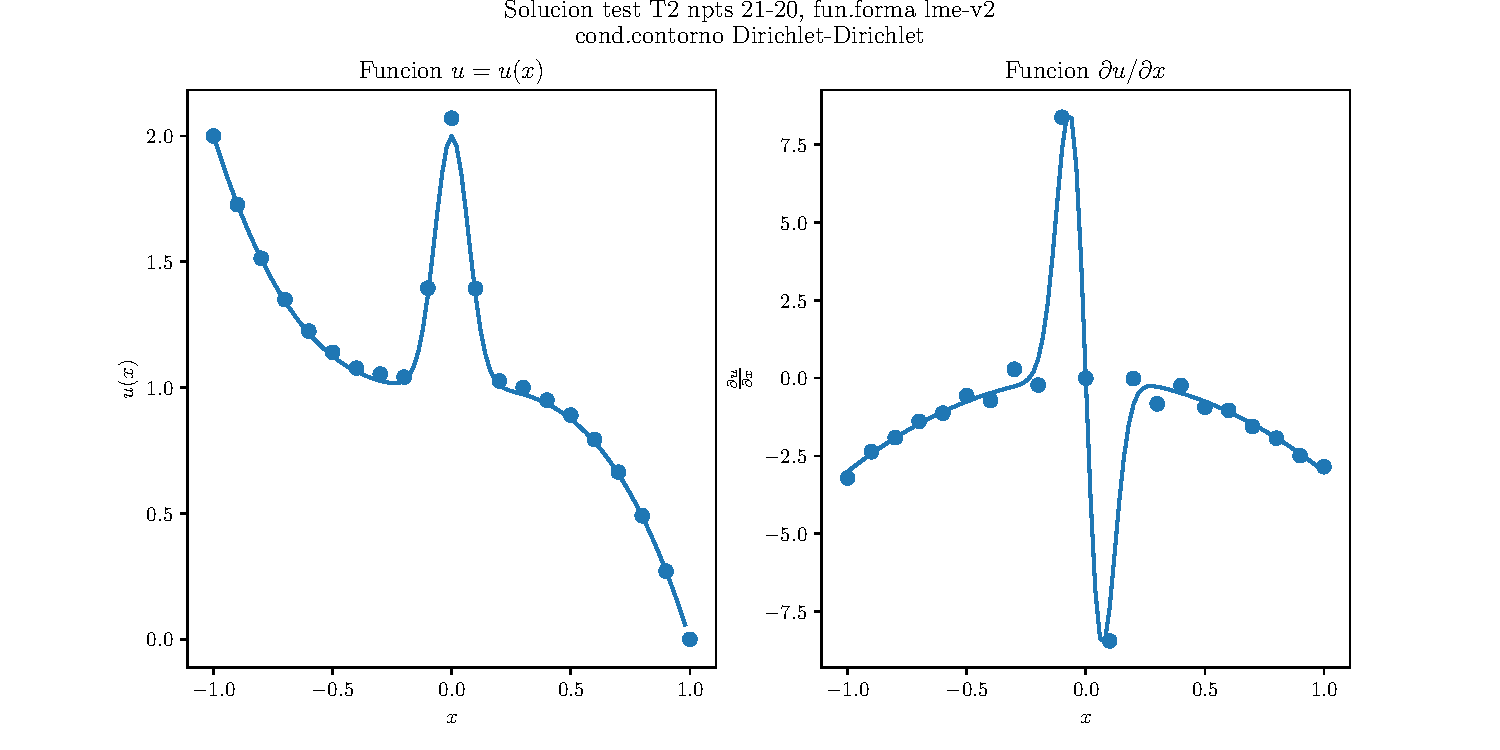
\includegraphics[width=1\textwidth]{./Imagenes/06/solucion/T2_21-20_regular_type-2_caso-1_lme-v2_direct_dgesv-lapack-blas.pdf}
    \caption{Solución del test T2} \label{fig:T2_caso-1_sol}
\end{figure}
%%%%%%%%%%%%%%%%%%%%%%%%%%%%%%%%%%%%%%%%%
\begin{figure}
    \centering
    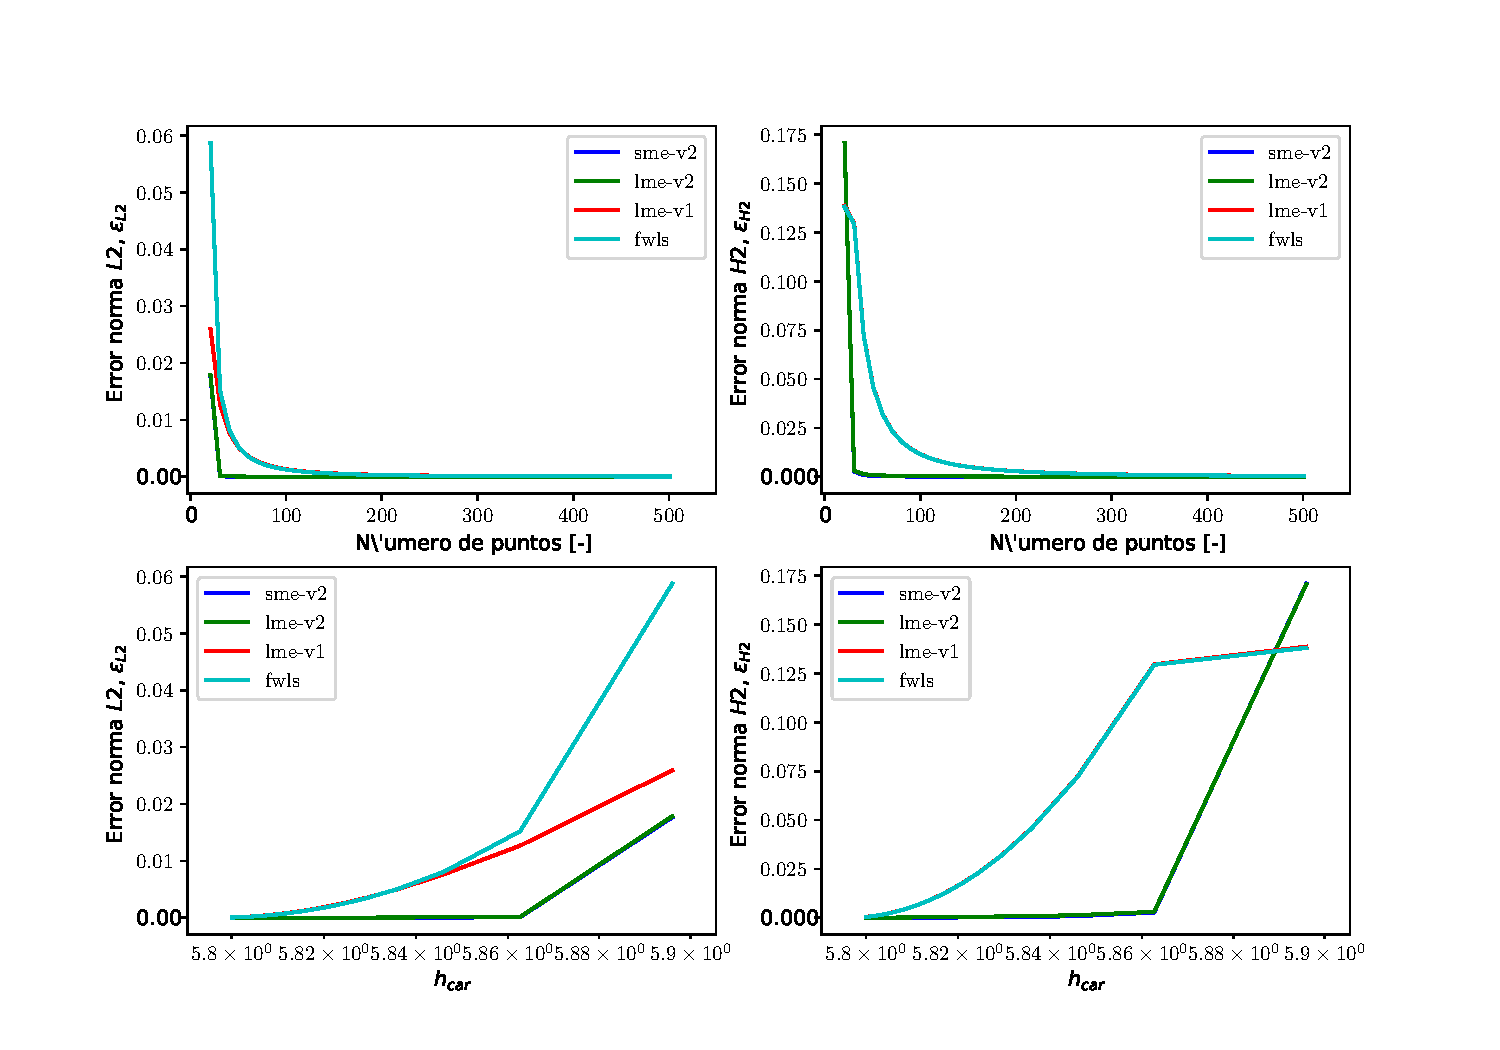
\includegraphics[width=1\textwidth]{./Imagenes/06/comparacion_shp_regular/T2_regular_type-2_caso-1_direct_dgesv-lapack-blas_sme-v2_lme-v2_lme-v1_fwls.pdf}
    \caption{Convergencia test T2 sujeto a condiciones Dirichlet - Dirichlet para una distribución regular} \label{fig:T2_caso-1_conv}
\end{figure}
\begin{figure}
    \centering
    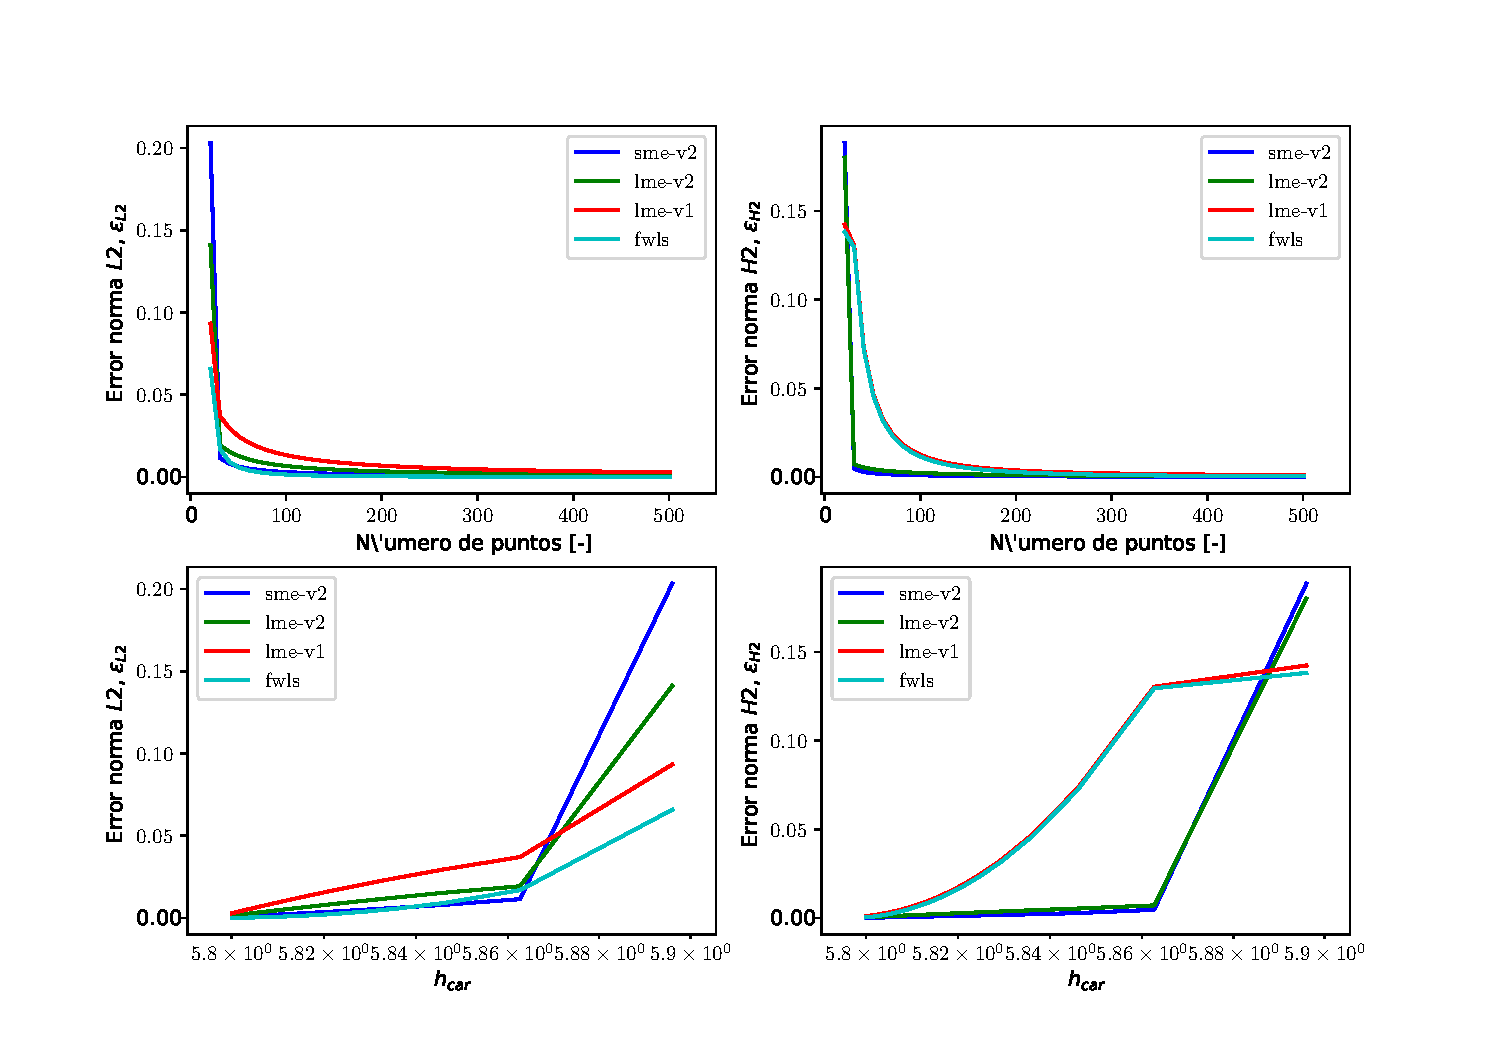
\includegraphics[width=1\textwidth]{./Imagenes/06/comparacion_shp_regular/T2_regular_type-2_caso-2_direct_dgesv-lapack-blas_sme-v2_lme-v2_lme-v1_fwls.pdf}
    \caption{Convergencia test T1 sujeto a condiciones Dirichlet - Neumann para una distribución regular} \label{fig:T2_caso-2_conv}
\end{figure}
\begin{figure}
    \centering
    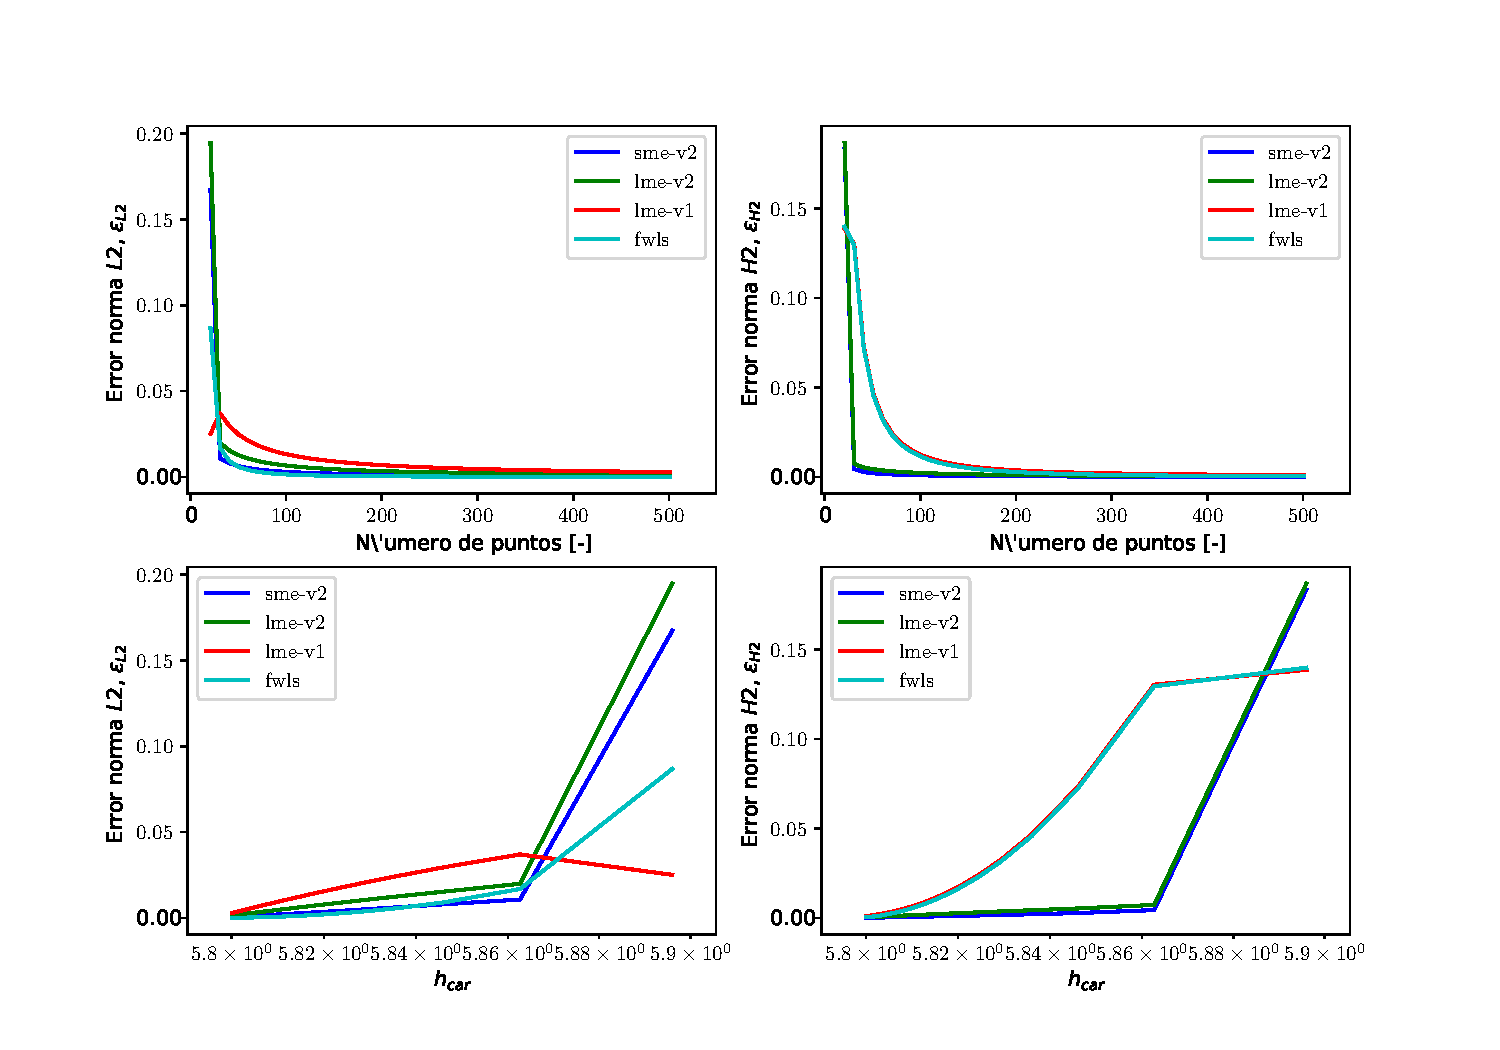
\includegraphics[width=1\textwidth]{./Imagenes/06/comparacion_shp_regular/T2_regular_type-2_caso-3_direct_dgesv-lapack-blas_sme-v2_lme-v2_lme-v1_fwls.pdf}
    \caption{Convergencia test T1 sujeto a condiciones Neumann - Dirichlet para una distribución regular} \label{fig:T2_caso-3_conv}
\end{figure}
%%%%%%%%%%%%%%%%%%%%%%%%%%%%%%%%%%%%%%%%%
\begin{figure}
    \centering
    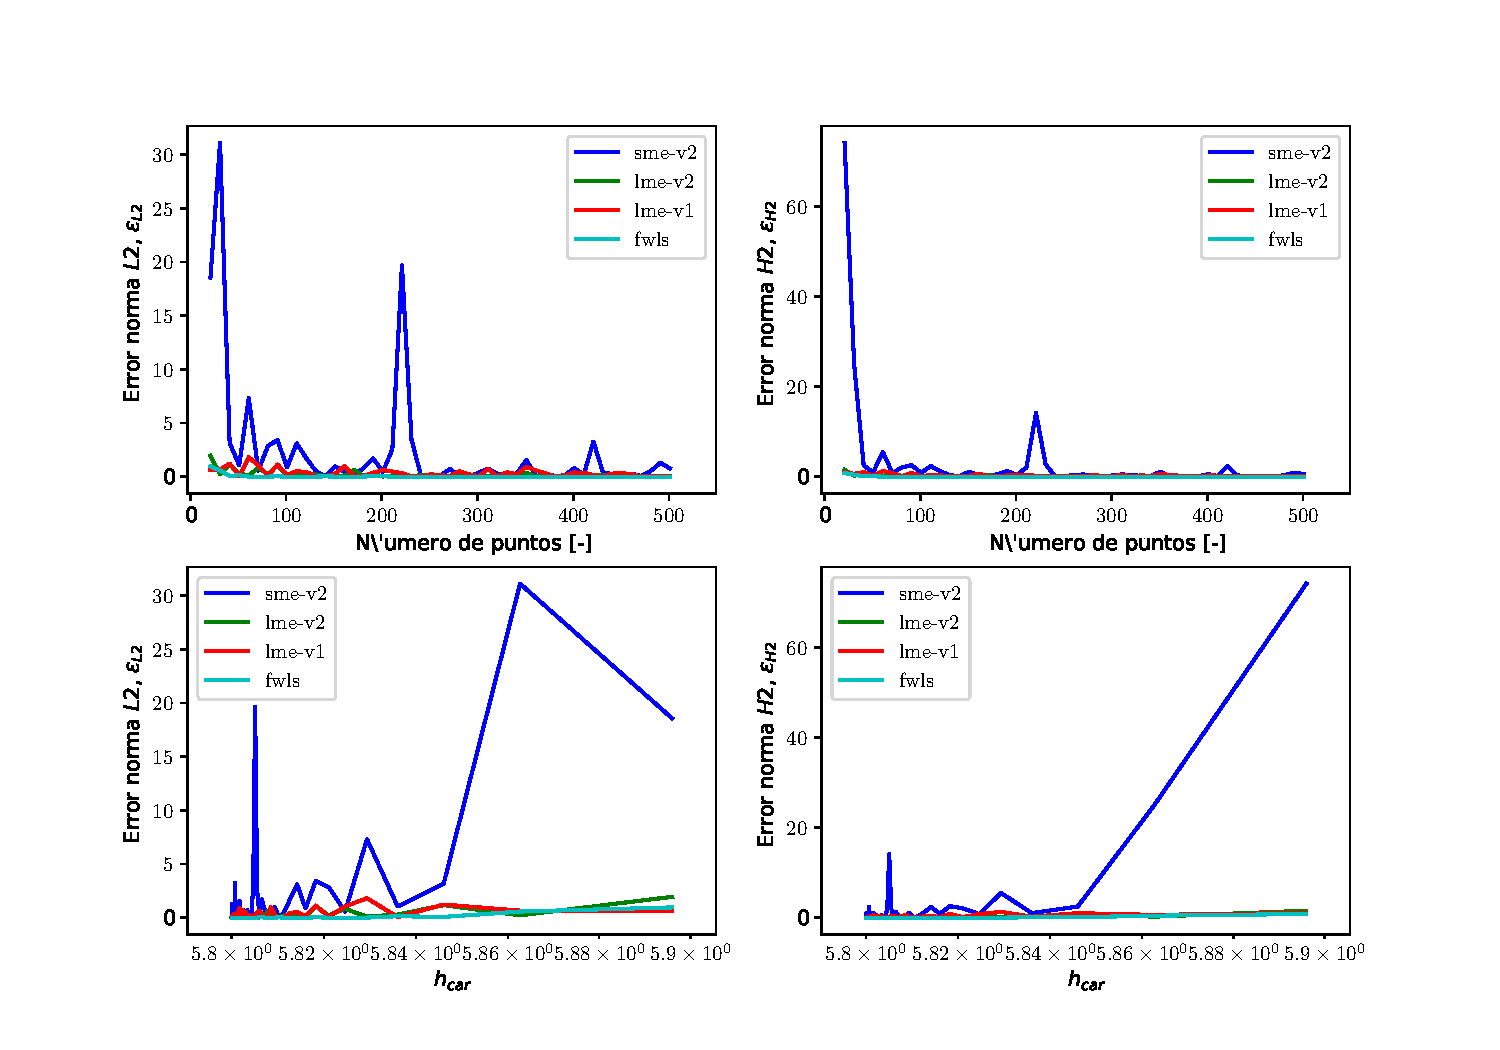
\includegraphics[width=1\textwidth]{./Imagenes/06/comparacion_shp_irreg/T2_irreg_type-2_caso-1_direct_dgesv-lapack-blas_sme-v2_lme-v2_lme-v1_fwls.pdf}
    \caption{Convergencia test T2 sujeto a condiciones Dirichlet - Dirichlet} \label{fig:T2_caso-1_conv_irreg}
\end{figure}
\begin{figure}
    \centering
    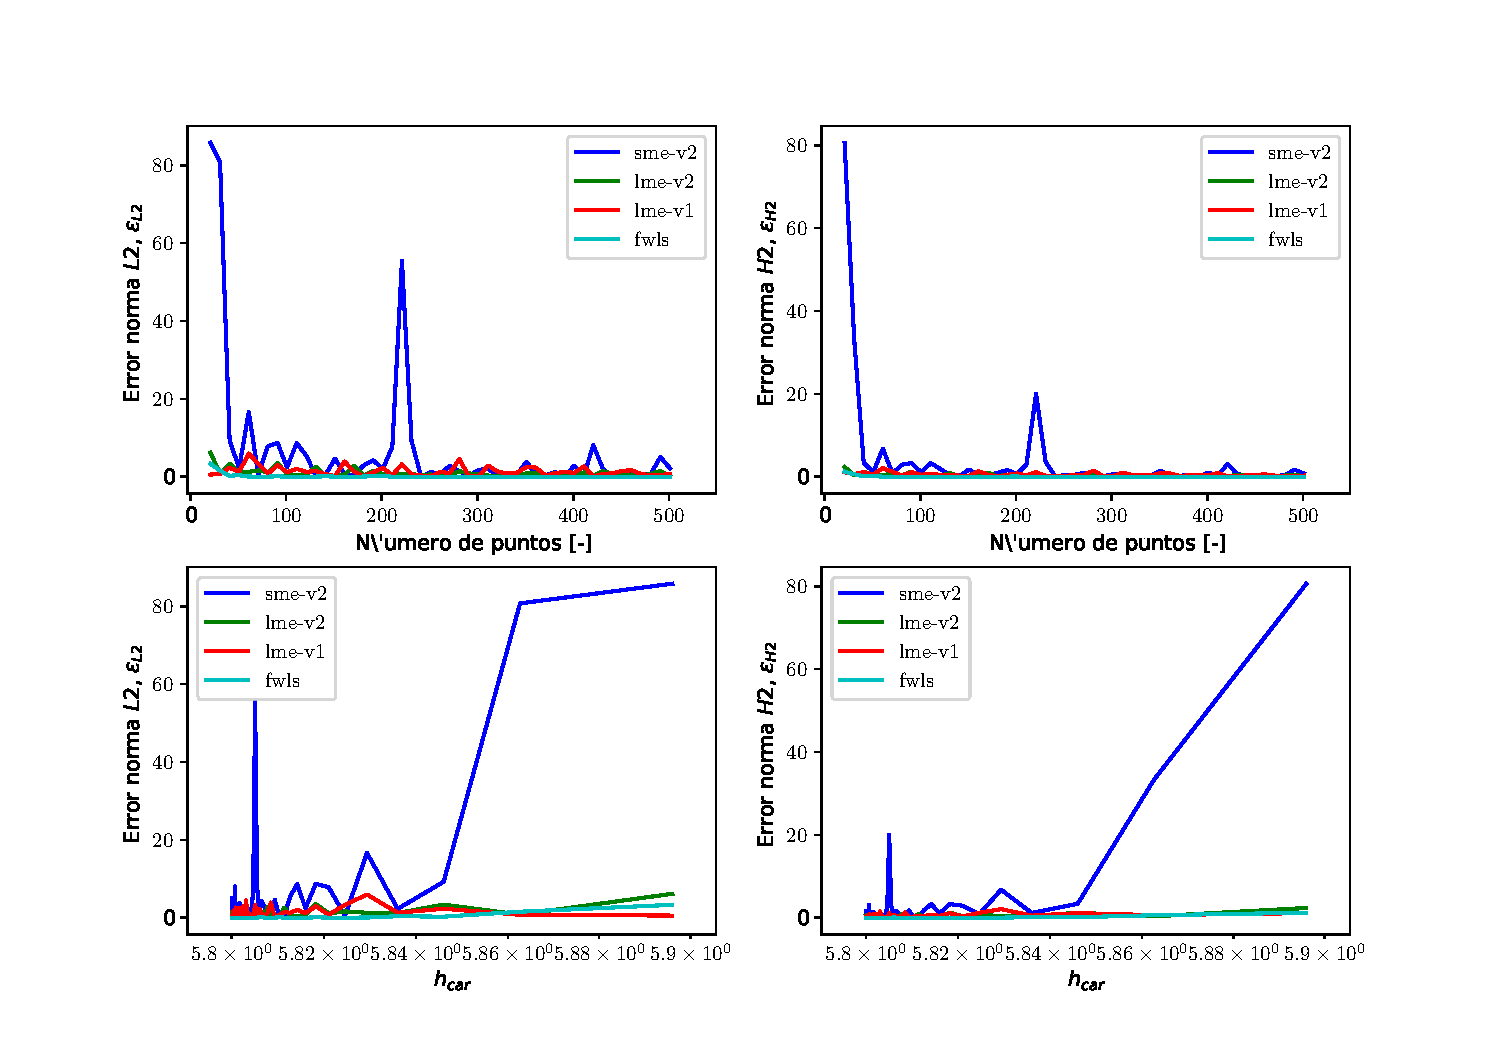
\includegraphics[width=1\textwidth]{./Imagenes/06/comparacion_shp_irreg/T2_irreg_type-2_caso-2_direct_dgesv-lapack-blas_sme-v2_lme-v2_lme-v1_fwls.pdf}
    \caption{Convergencia test T1 sujeto a condiciones Dirichlet - Neumann} \label{fig:T2_caso-2_conv_irreg}
\end{figure}
\begin{figure}
    \centering
    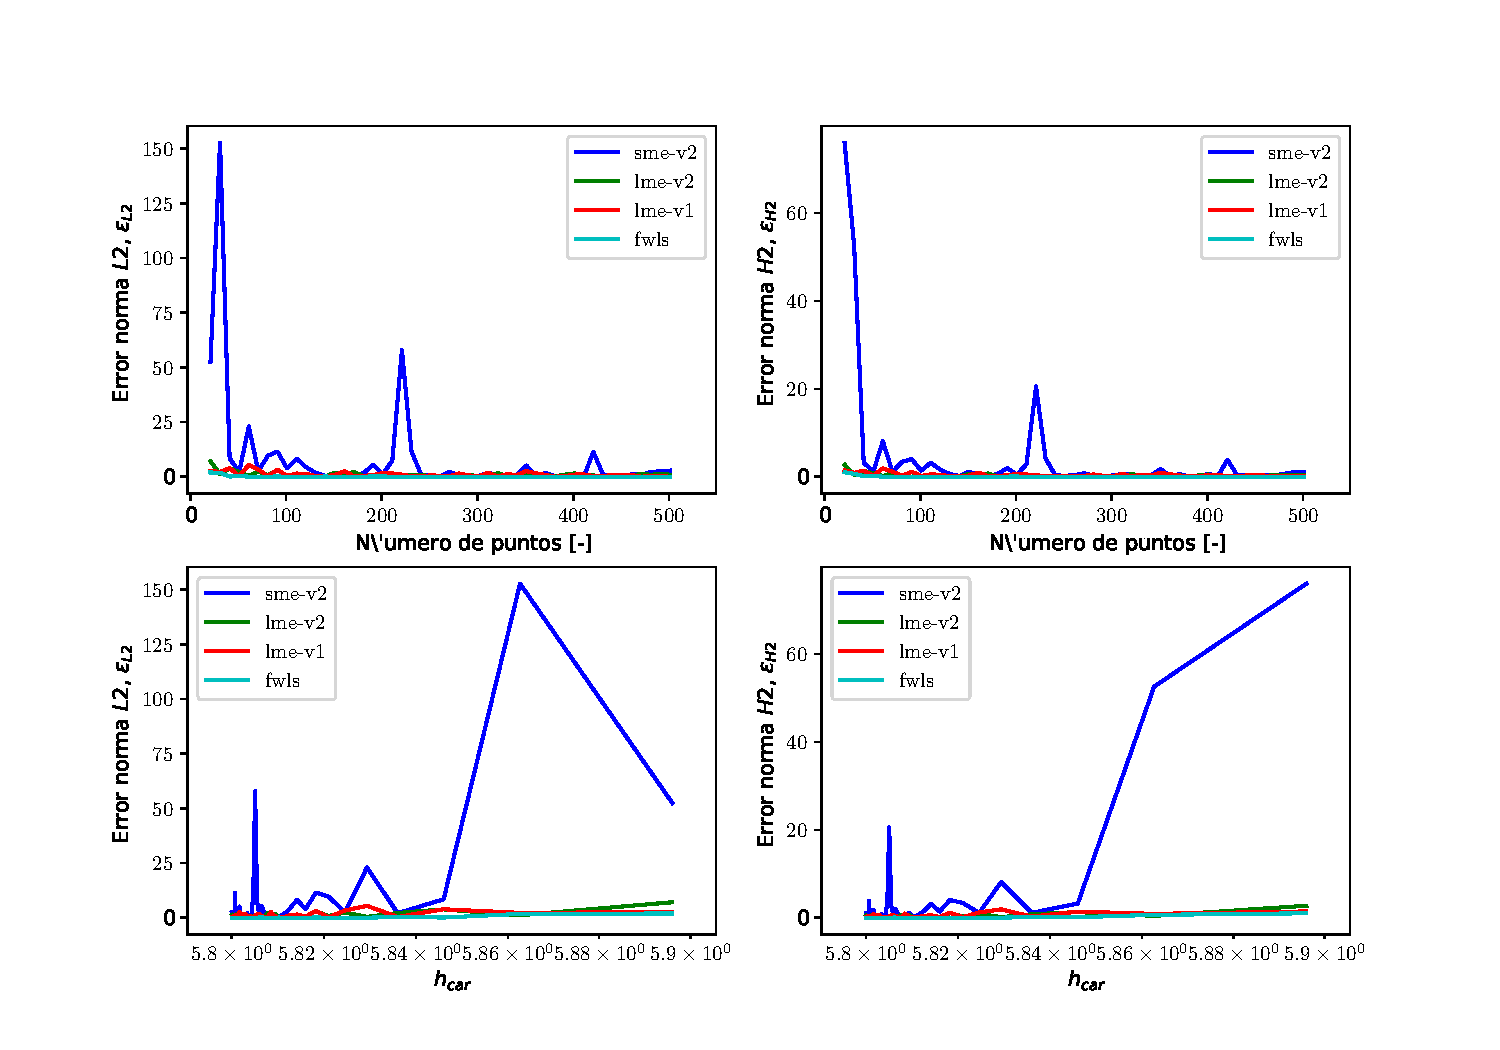
\includegraphics[width=1\textwidth]{./Imagenes/06/comparacion_shp_irreg/T2_irreg_type-2_caso-3_direct_dgesv-lapack-blas_sme-v2_lme-v2_lme-v1_fwls.pdf}
    \caption{Convergencia test T1 sujeto a condiciones Neumann - Dirichlet} \label{fig:T2_caso-3_conv_irreg}
\end{figure}

%%%%%%%%%%%%%%%%%%%%%%%%%%%%%%%%%%%%%%%%%%%%%%%%%%%%%%%%%%%%%%%%%%%%

\subsection{ElasticBar}
Se tiene una barra elastica lineal que sujeta a una fuerza de tracción la cual se encuentra en equilibrio. La ecuación governante está dada por:
\begin{equation}
    \frac{d^2}{dx^2} + b = 0
\end{equation}
\begin{eqnarray}
    u = \frac{1}{E} ( \frac{1}{2} x - \frac{x^3}{6})
    du = \frac{( 1 -x^2 )}{2}
\end{eqnarray}
En la Figura \ref{fig:ElasticBar_caso-1_sol} se muestra la solución y en las Figuras \ref{fig:ElasticBar_caso-1_conv} \ref{fig:ElasticBar_caso-2_conv} \ref{fig:ElasticBar_caso-3_conv} se muestra la convergencia de la solución
\begin{figure}
    \centering
    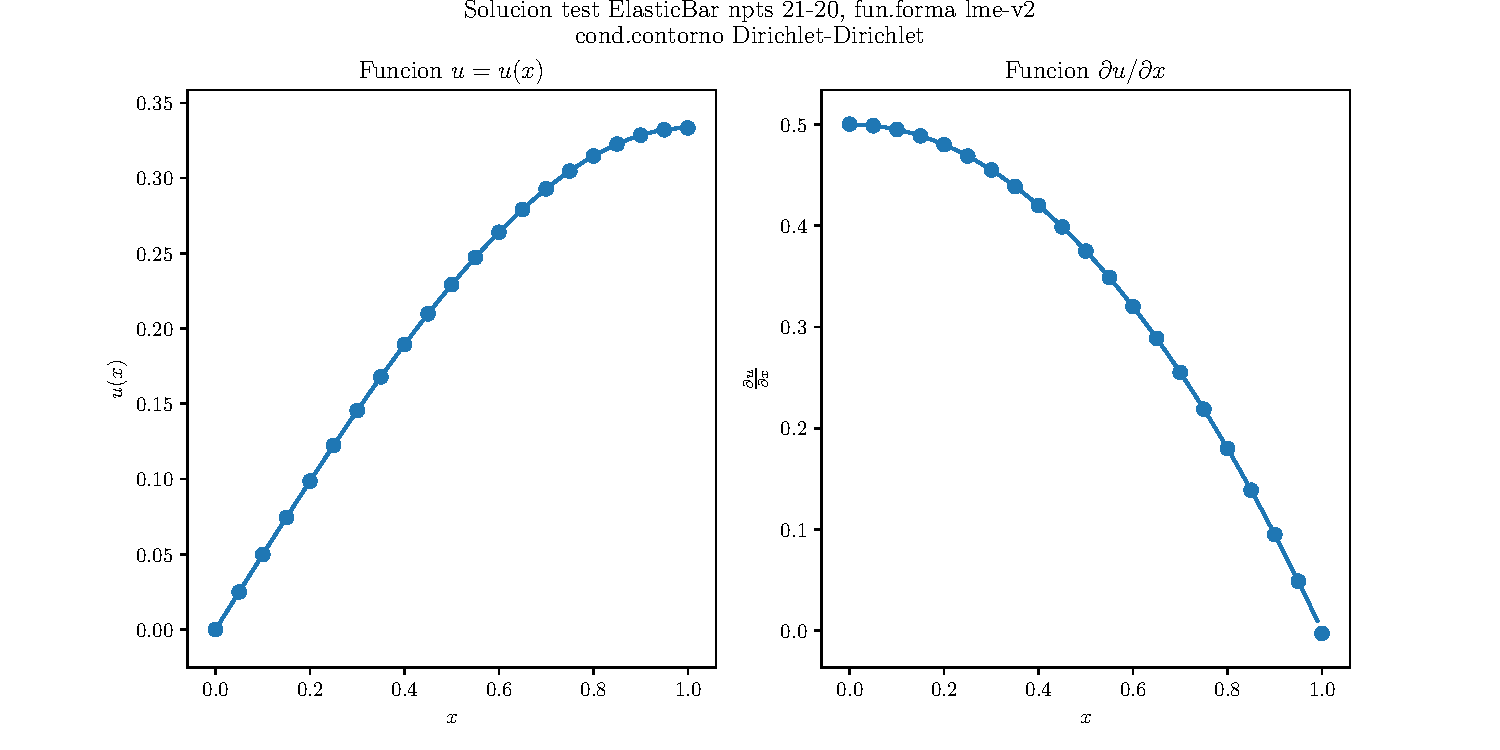
\includegraphics[width=1\textwidth]{./Imagenes/06/solucion/ElasticBar_21-20_regular_type-2_caso-1_lme-v2_direct_dgesv-lapack-blas.pdf}
    \caption{Solución del test ElasticBar} \label{fig:ElasticBar_caso-1_sol}
\end{figure}
%%%%%%%%%%%%%%%%%%%%%%%%%%%%%%%%%%%%%%%%%
\begin{figure}
    \centering
    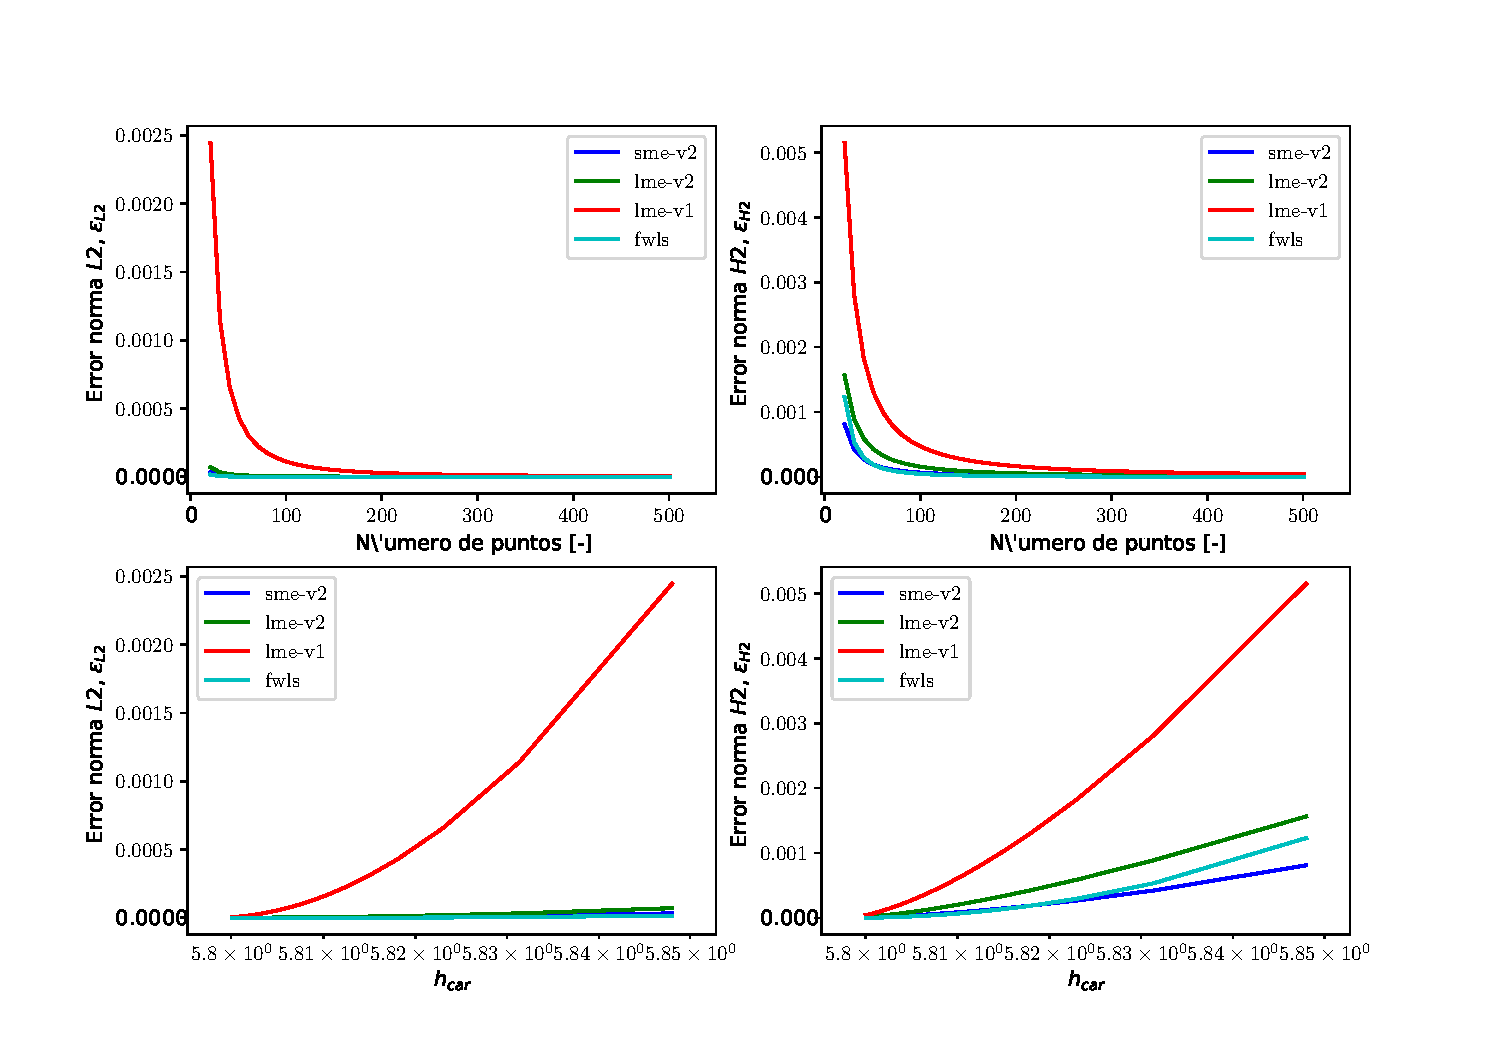
\includegraphics[width=1\textwidth]{./Imagenes/06/comparacion_shp_regular/ElasticBar_regular_type-2_caso-1_direct_dgesv-lapack-blas_sme-v2_lme-v2_lme-v1_fwls.pdf}
    \caption{Convergencia test ElasticBar sujeto a condiciones Dirichlet - Dirichlet para una distribución regular} \label{fig:ElasticBar_caso-1_conv}
\end{figure}
\begin{figure}
    \centering
    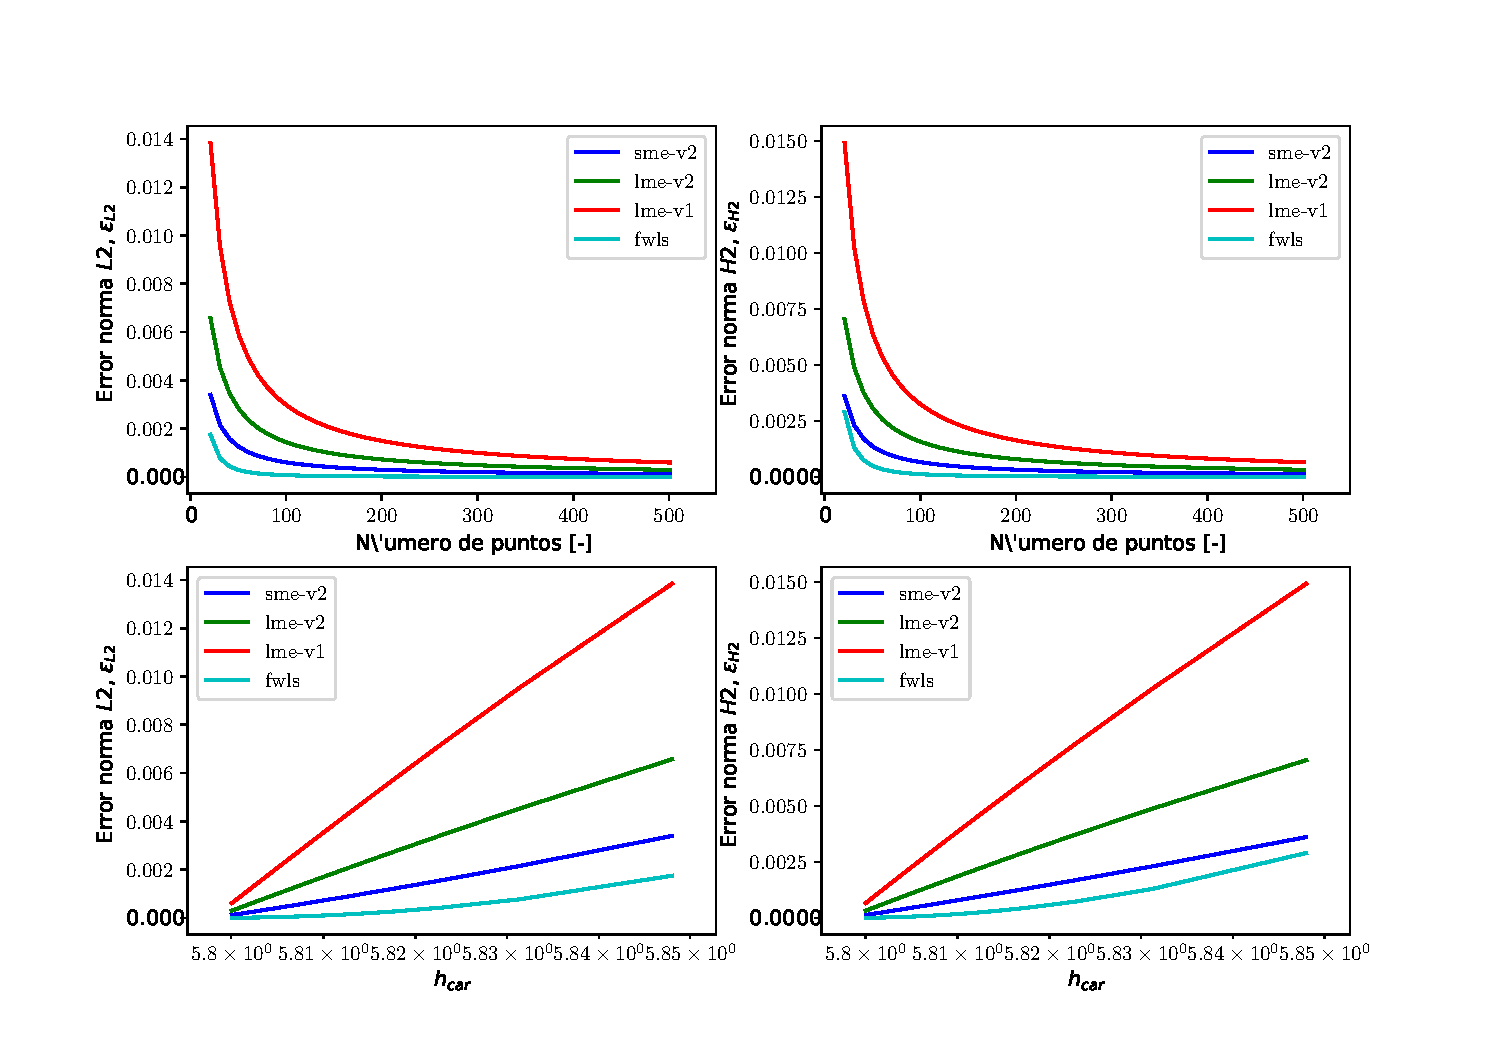
\includegraphics[width=1\textwidth]{./Imagenes/06/comparacion_shp_regular/ElasticBar_regular_type-2_caso-2_direct_dgesv-lapack-blas_sme-v2_lme-v2_lme-v1_fwls.pdf}
    \caption{Convergencia test ElasticBar sujeto a condiciones Dirichlet - Neumann para una distribución regular} \label{fig:ElasticBar_caso-2_conv}
\end{figure}
\begin{figure}
    \centering
    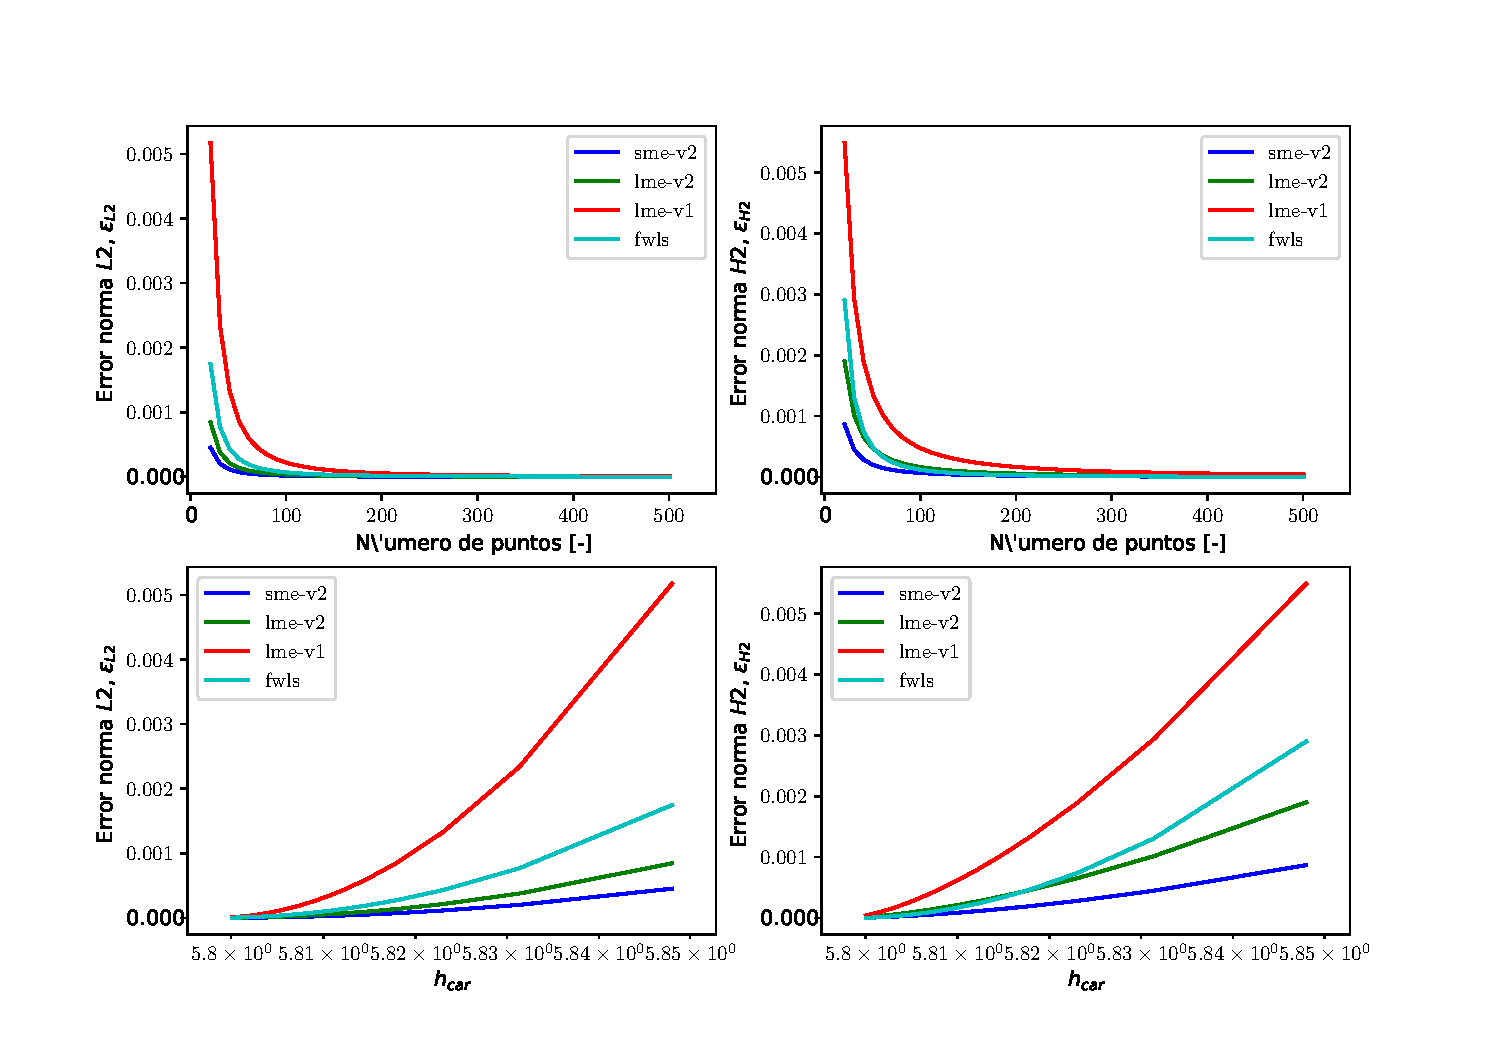
\includegraphics[width=1\textwidth]{./Imagenes/06/comparacion_shp_regular/ElasticBar_regular_type-2_caso-3_direct_dgesv-lapack-blas_sme-v2_lme-v2_lme-v1_fwls.pdf}
    \caption{Convergencia test ElasticBar sujeto a condiciones Neumann - Dirichlet para una distribución regular} \label{fig:ElasticBar_caso-3_conv}
\end{figure}
%%%%%%%%%%%%%%%%%%%%%%%%%%%%%%%%%%%%%%%%%
\begin{figure}
    \centering
    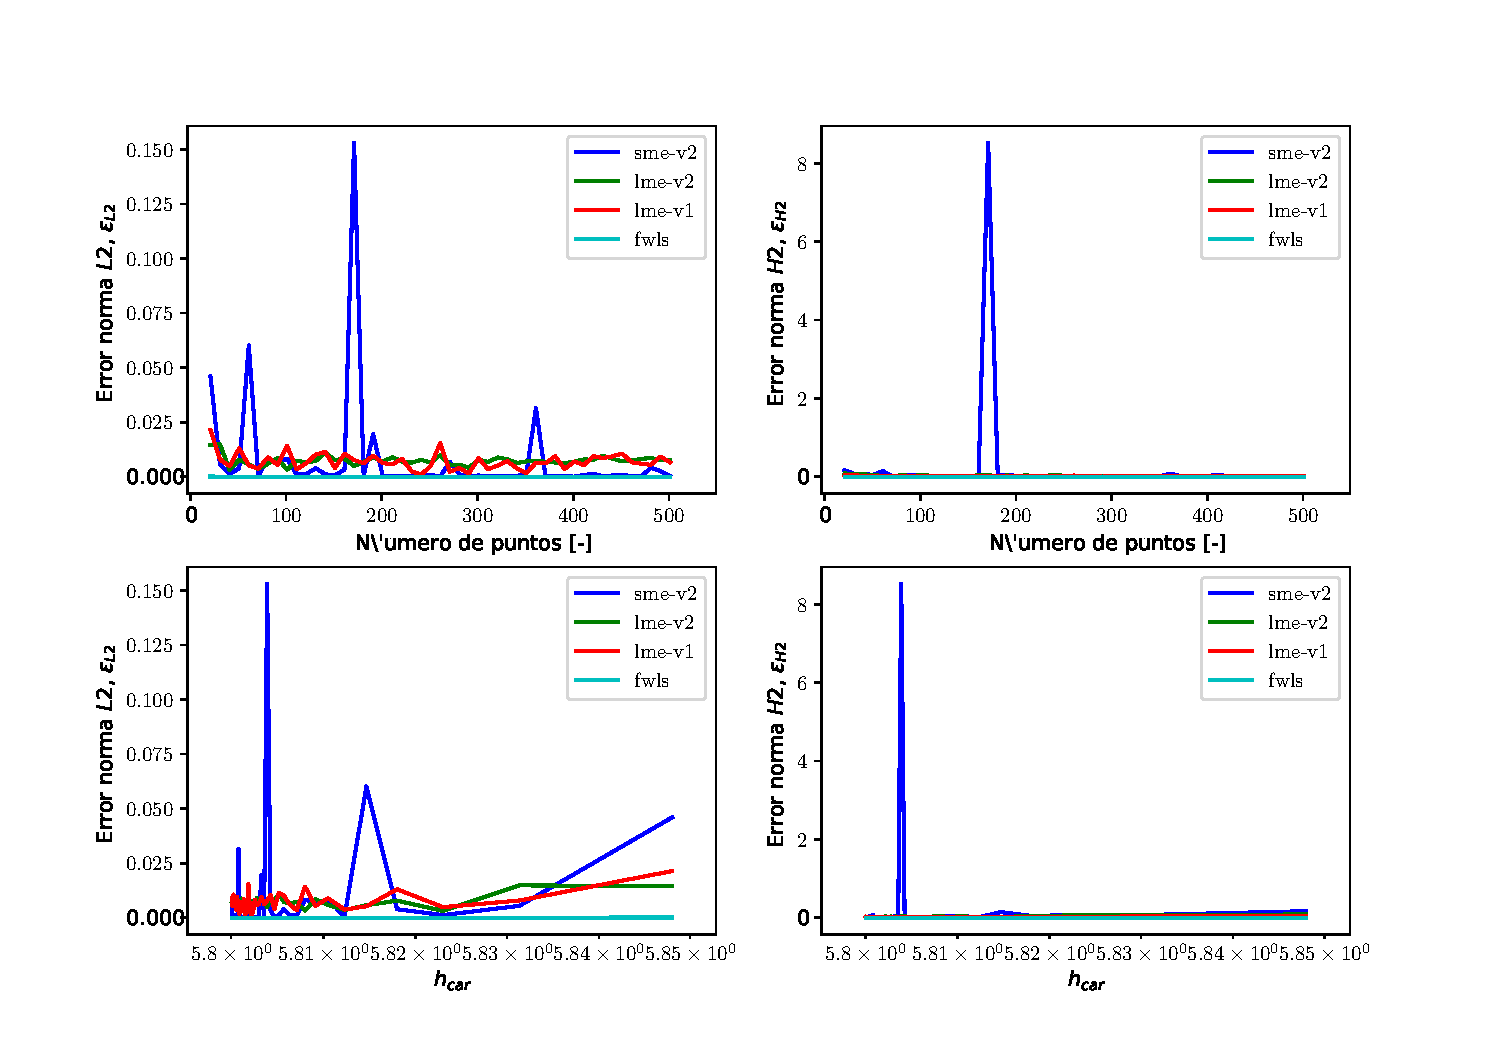
\includegraphics[width=1\textwidth]{./Imagenes/06/comparacion_shp_irreg/ElasticBar_irreg_type-2_caso-1_direct_dgesv-lapack-blas_sme-v2_lme-v2_lme-v1_fwls.pdf}
    \caption{Convergencia test ElasticBar sujeto a condiciones Dirichlet - Dirichlet} \label{fig:ElasticBar_caso-1_conv_irreg}
\end{figure}
\begin{figure}
    \centering
    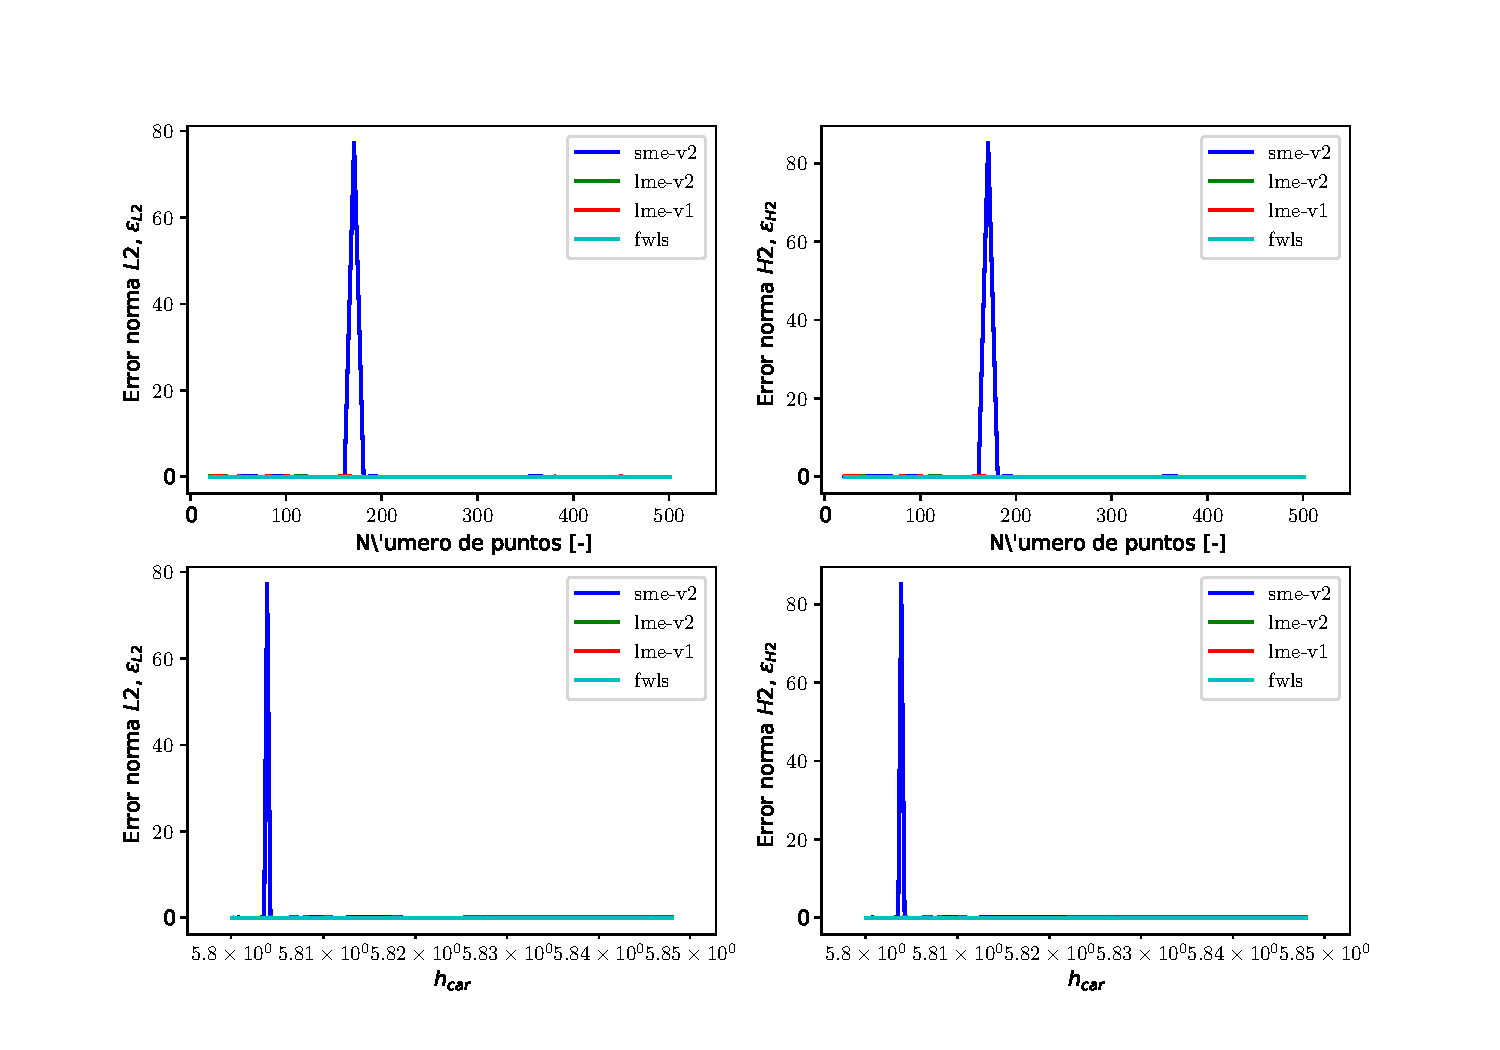
\includegraphics[width=1\textwidth]{./Imagenes/06/comparacion_shp_irreg/ElasticBar_irreg_type-2_caso-2_direct_dgesv-lapack-blas_sme-v2_lme-v2_lme-v1_fwls.pdf}
    \caption{Convergencia test ElasticBar sujeto a condiciones Dirichlet - Neumann} \label{fig:ElasticBar_caso-2_conv_irreg}
\end{figure}
\begin{figure}
    \centering
    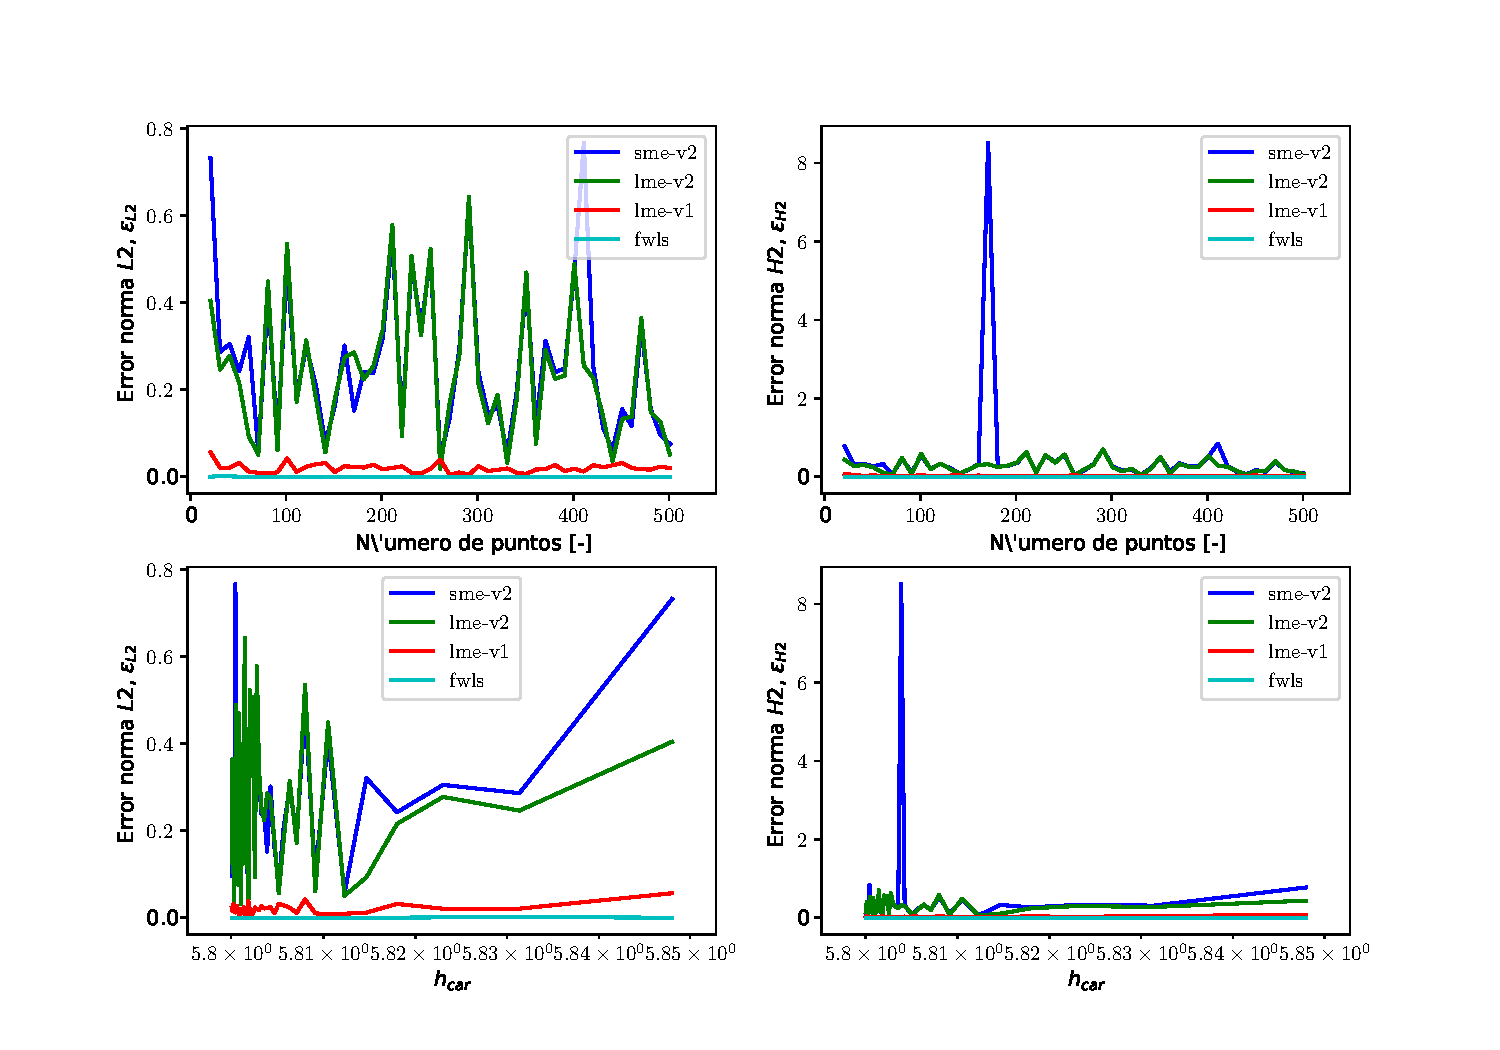
\includegraphics[width=1\textwidth]{./Imagenes/06/comparacion_shp_irreg/ElasticBar_irreg_type-2_caso-3_direct_dgesv-lapack-blas_sme-v2_lme-v2_lme-v1_fwls.pdf}
    \caption{Convergencia test ElasticBar sujeto a condiciones Neumann - Dirichlet} \label{fig:ElasticBar_caso-3_conv_irreg}
\end{figure}

%%%%%%%%%%%%%%%%%%%%%%%%%%%%%%%%%%%%%%%%%%%%%%%%%%%%%%%%%%%%%%%%%%%%

\subsection{Rachford Wheeler}
cuya solución exacta es
\begin{equation}
    --\frac{d^2u}{dx^2} + u = f(x) 
\end{equation}
sujeto a,
\begin{equation}
    \frac{du}{dx}|_{x=0} = \frac{\alpha}{1+\alpha^2 \overline{x}^2} 
\end{equation}
\begin{eqnarray}
    u  = ( 1-x ) (\arctan(a(x-xo))+\arctan(a xo)) \\
    du = ( 1-x ) \frac{a}{( 1 + a^2 (x-xo)^2 )} - \arctan(a (x-xo)) + \arctan(a xo)
\end{eqnarray}
En la Figura \ref{fig:RW_caso-1_sol} se grafica la solución numérica. En las Figuras \ref{fig:RW_caso-1_conv} \ref{fig:RW_caso-2_conv} \ref{fig:RW_caso-3_conv} se muestra la convergencia de la solución
\begin{figure}
    \centering
    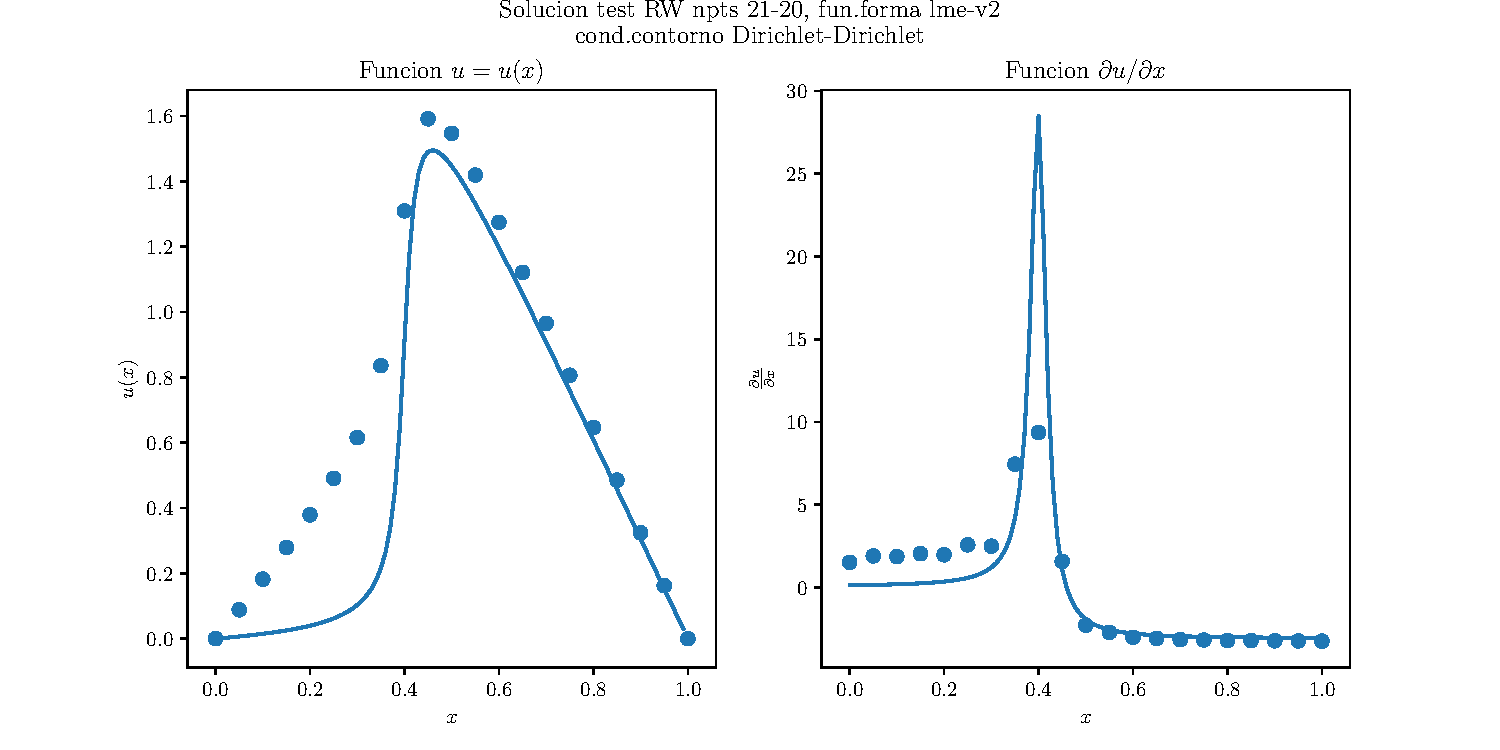
\includegraphics[width=1\textwidth]{./Imagenes/06/solucion/RW_21-20_regular_type-2_caso-1_lme-v2_direct_dgesv-lapack-blas.pdf}
    \caption{Solución del test RW} \label{fig:RW_caso-1_sol}
\end{figure}
%%%%%%%%%%%%%%%%%%%%%%%%%%%%%%%%%%%%%%%%%
\begin{figure}
    \centering
    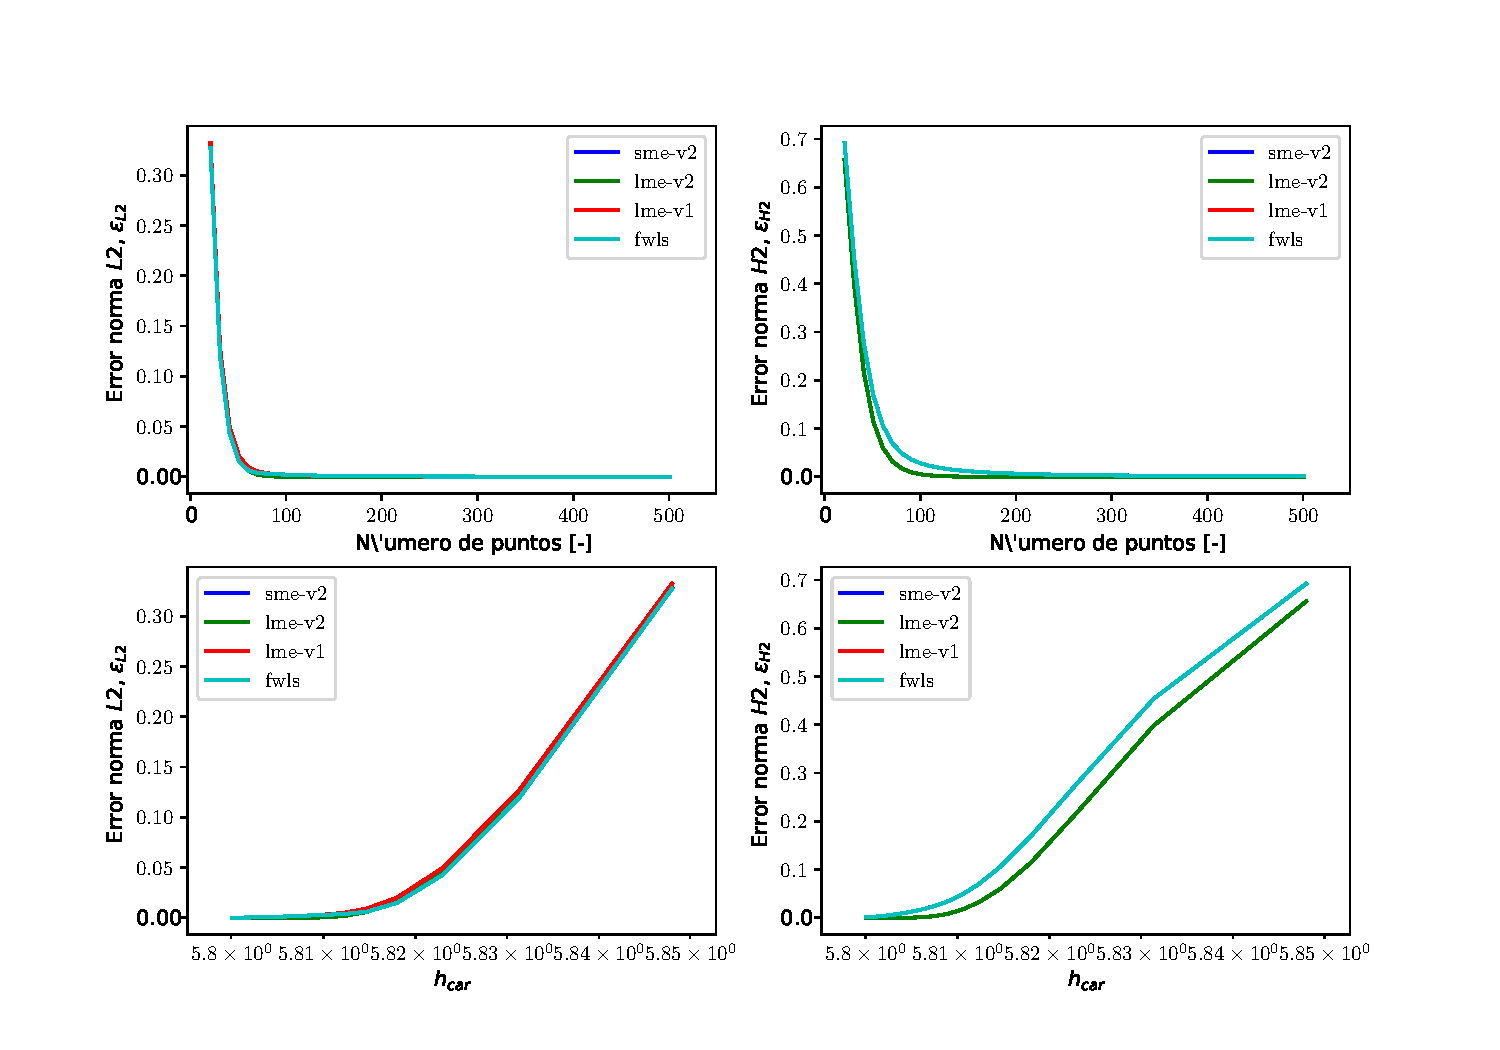
\includegraphics[width=1\textwidth]{./Imagenes/06/comparacion_shp_regular/RW_regular_type-2_caso-1_direct_dgesv-lapack-blas_sme-v2_lme-v2_lme-v1_fwls.pdf}
    \caption{Convergencia test RW sujeto a condiciones Dirichlet - Dirichlet para una distribución regular} \label{fig:RW_caso-1_conv}
\end{figure}
\begin{figure}
    \centering
    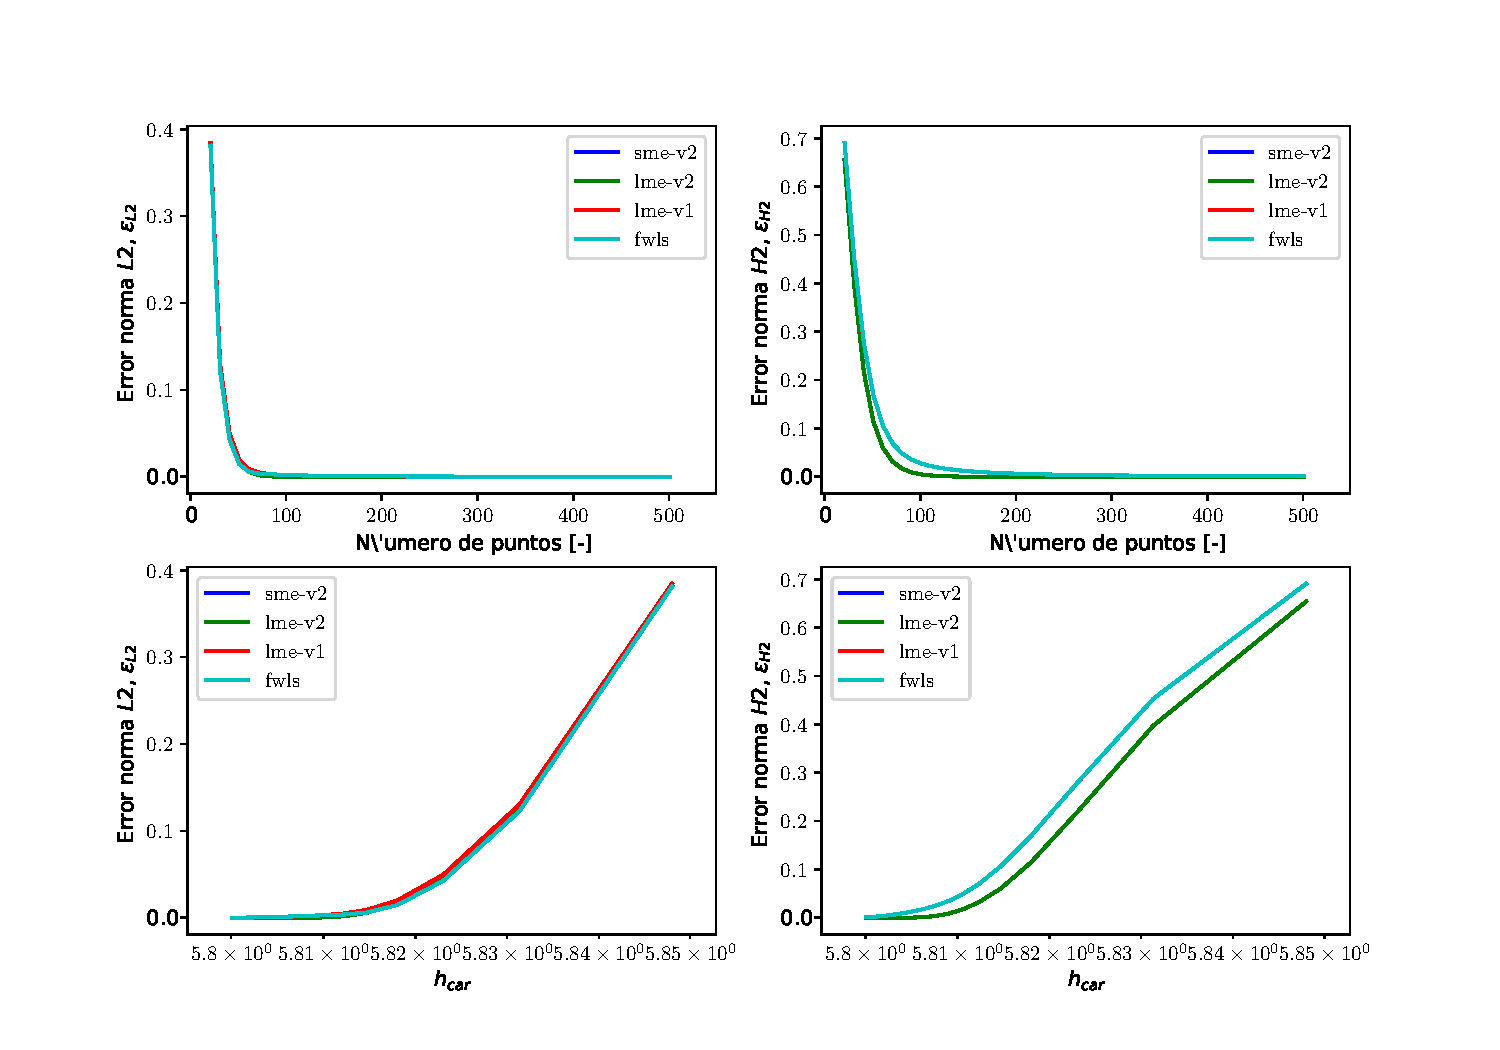
\includegraphics[width=1\textwidth]{./Imagenes/06/comparacion_shp_regular/RW_regular_type-2_caso-2_direct_dgesv-lapack-blas_sme-v2_lme-v2_lme-v1_fwls.pdf}
    \caption{Convergencia test RW sujeto a condiciones Dirichlet - Neumann para una distribución regular} \label{fig:RW_caso-2_conv}
\end{figure}
\begin{figure}
    \centering
    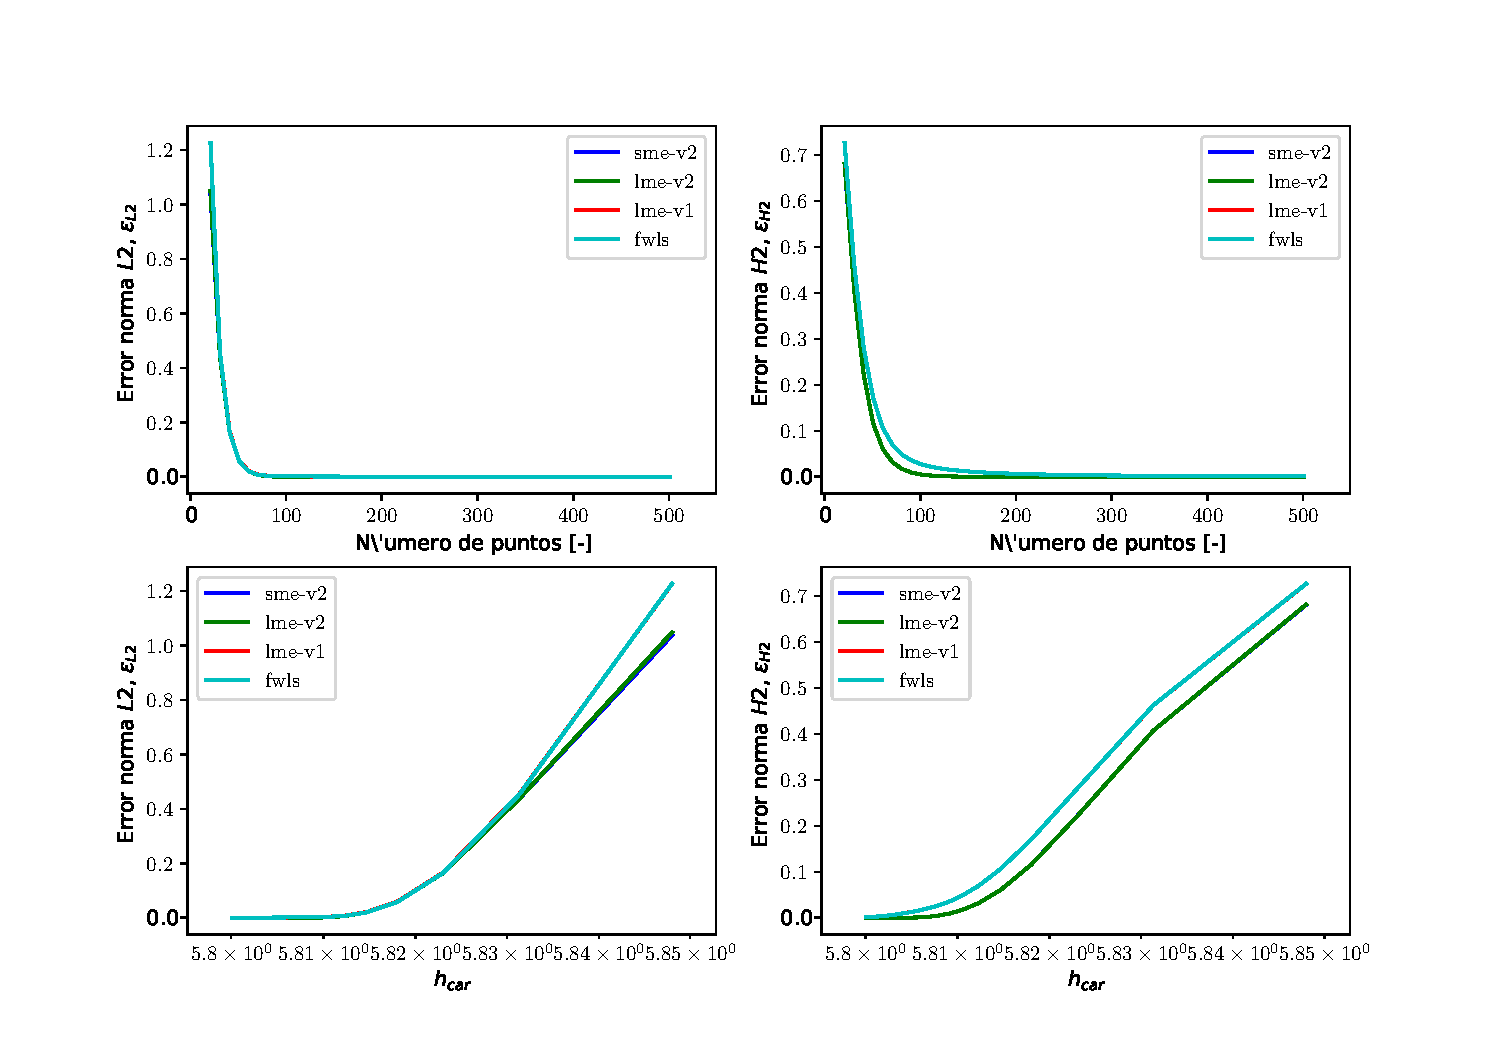
\includegraphics[width=1\textwidth]{./Imagenes/06/comparacion_shp_regular/RW_regular_type-2_caso-3_direct_dgesv-lapack-blas_sme-v2_lme-v2_lme-v1_fwls.pdf}
    \caption{Convergencia test RW sujeto a condiciones Neumann - Dirichlet para una distribución regular} \label{fig:RW_caso-3_conv}
\end{figure}
%%%%%%%%%%%%%%%%%%%%%%%%%%%%%%%%%%%%%%%%%
\begin{figure}
    \centering
    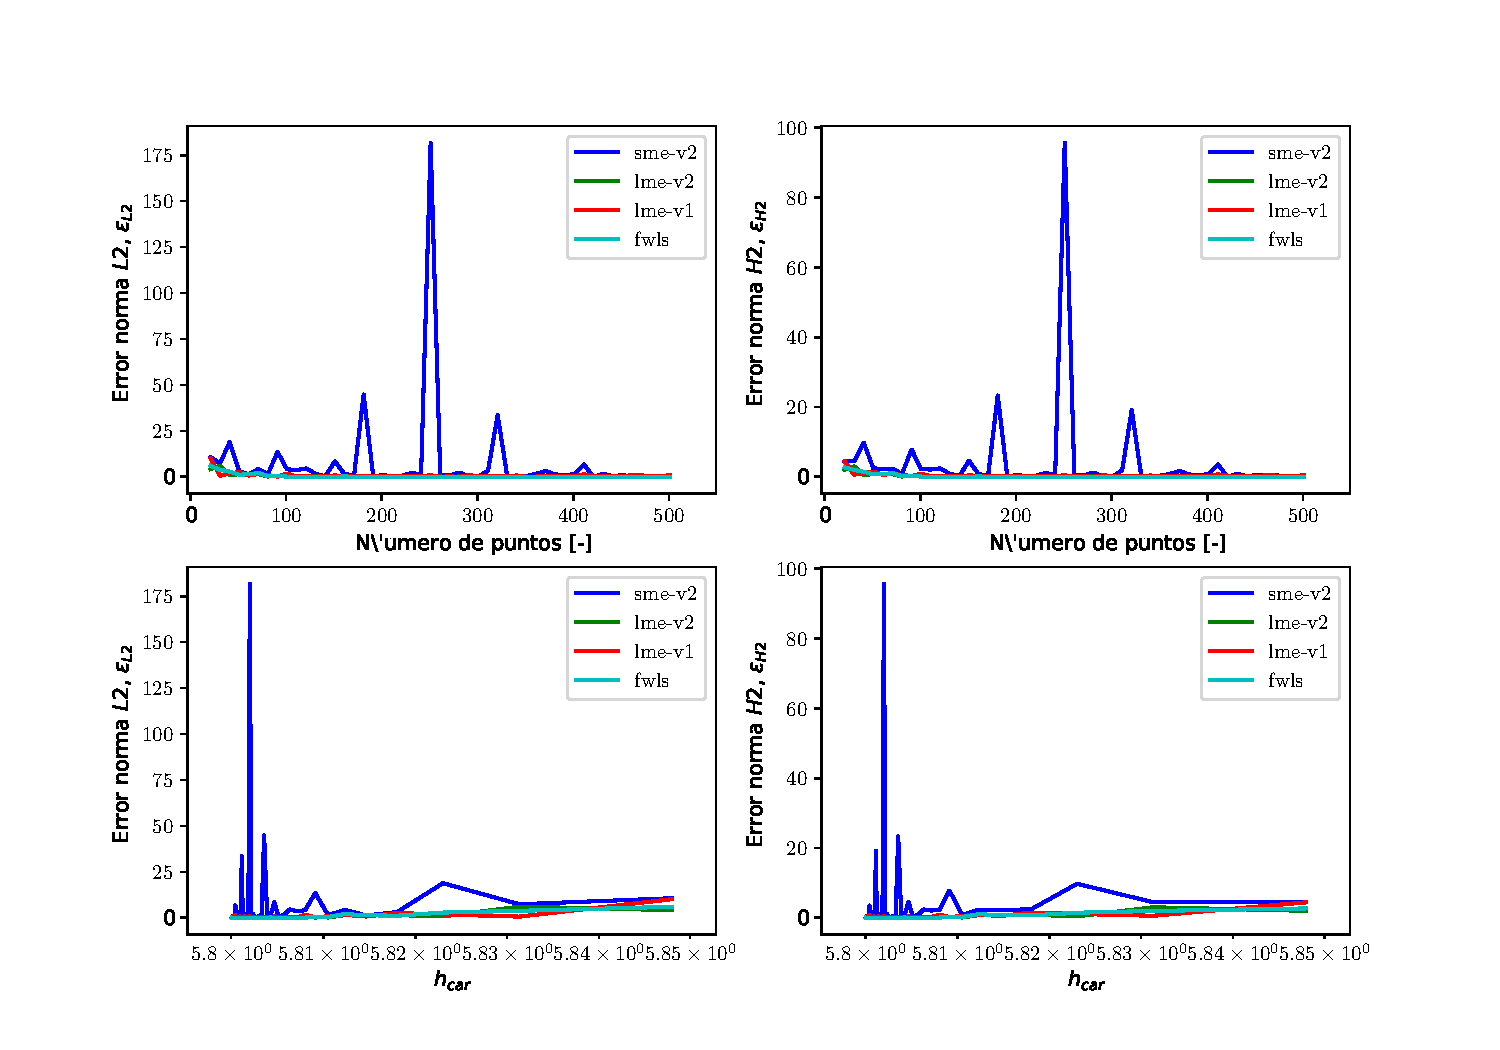
\includegraphics[width=1\textwidth]{./Imagenes/06/comparacion_shp_irreg/RW_irreg_type-2_caso-1_direct_dgesv-lapack-blas_sme-v2_lme-v2_lme-v1_fwls.pdf}
    \caption{Convergencia test RW sujeto a condiciones Dirichlet - Dirichlet para una distribución irregular} \label{fig:RW_caso-1_conv}
\end{figure}
\begin{figure}
    \centering
    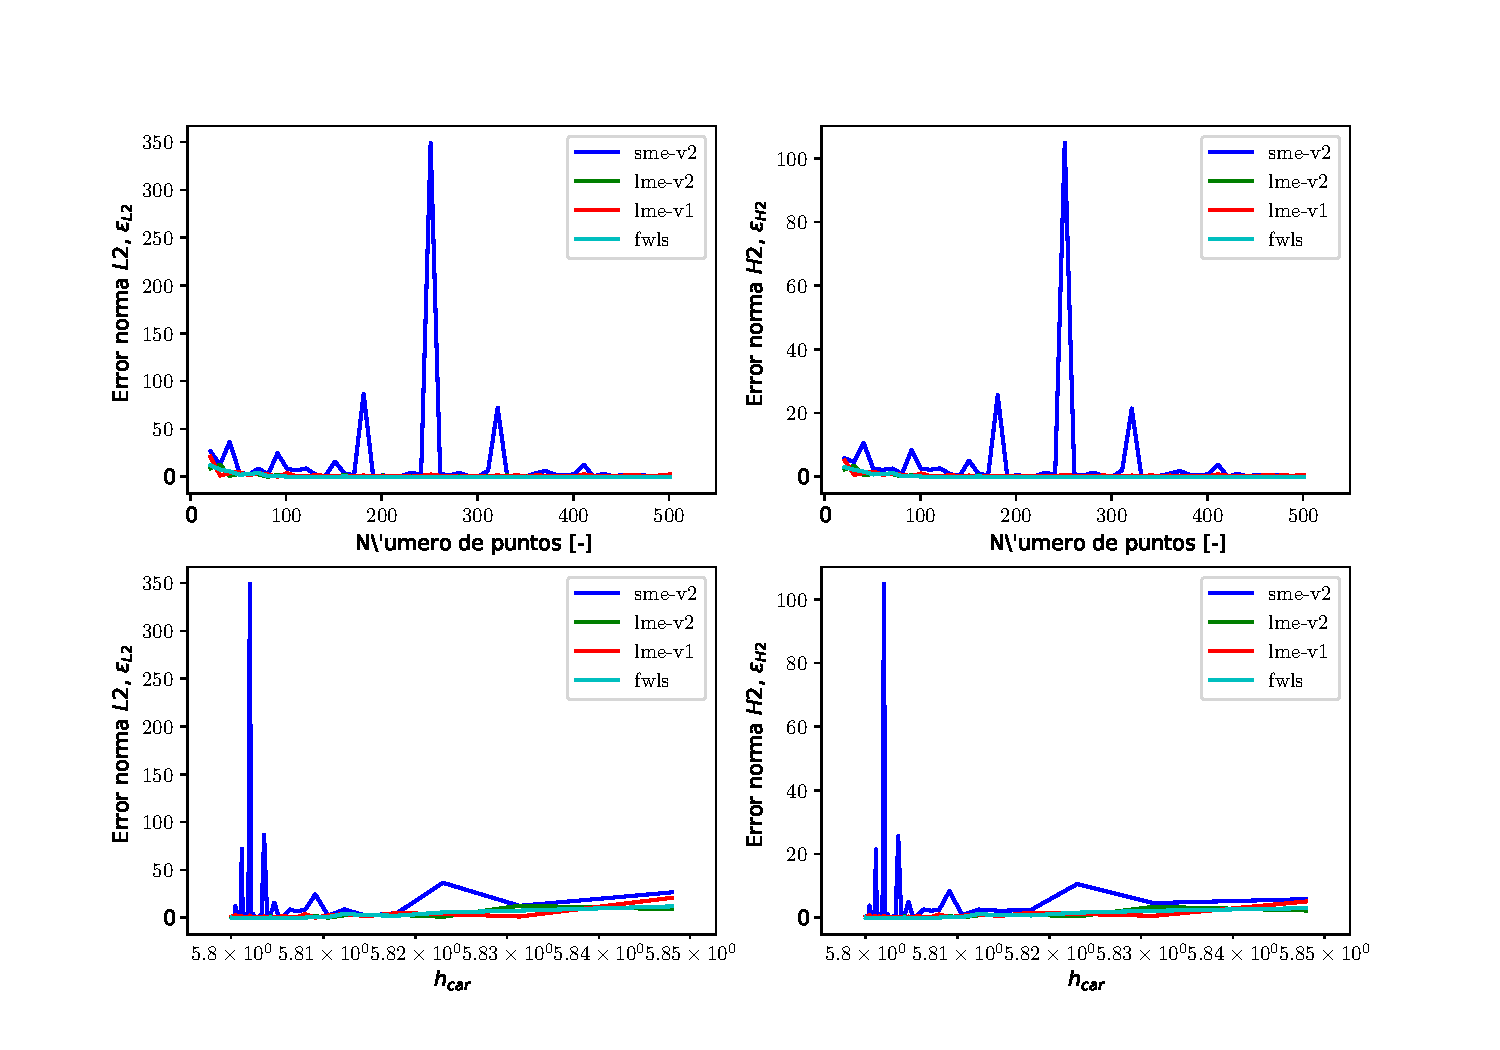
\includegraphics[width=1\textwidth]{./Imagenes/06/comparacion_shp_irreg/RW_irreg_type-2_caso-2_direct_dgesv-lapack-blas_sme-v2_lme-v2_lme-v1_fwls.pdf}
    \caption{Convergencia test RW sujeto a condiciones Dirichlet - Neumann para una distribución irregular} \label{fig:RW_caso-2_conv}
\end{figure}
\begin{figure}
    \centering
    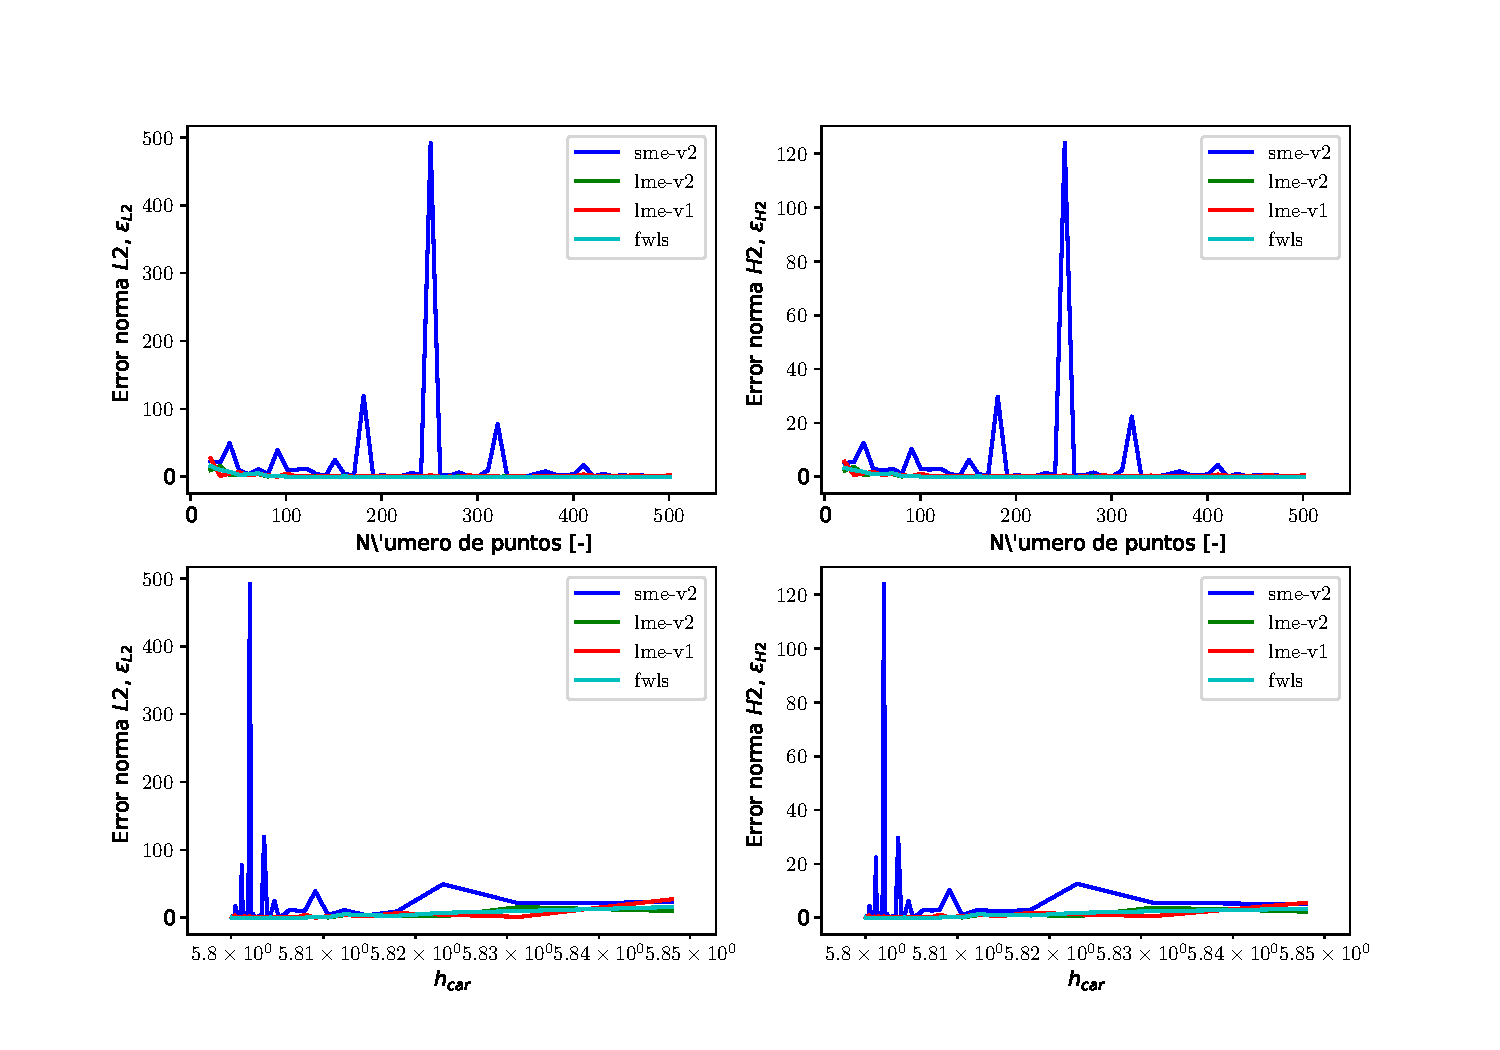
\includegraphics[width=1\textwidth]{./Imagenes/06/comparacion_shp_irreg/RW_irreg_type-2_caso-3_direct_dgesv-lapack-blas_sme-v2_lme-v2_lme-v1_fwls.pdf}
    \caption{Convergencia test RW sujeto a condiciones Neumann - Dirichlet para una distribución irregular} \label{fig:RW_caso-3_conv}
\end{figure}

%%%%%%%%%%%%%%%%%%%%%%%%%%%%%%%%%%%%%%%%%%%%%%%%%%%%%%%%%%%%%%%%%%%%

\subsection{AxialTruss}
La ecuación governante es
\begin{equation}
    E A \frac{d^2 u}{d^2 x} + b(x) = 0
\end{equation}
y su término fuente es:
\begin{equation}
    b(x) = -(2.3 \pi)^2 \sin(2.3\pi x)
\end{equation}
donde su extremo izquierdo ($x=0$) se encuentra fijo y su extremo derecho ($x=1$) se le aplica una fuerza sinusoidal a lo largo del eje $x$, es decir:
\begin{equation}
    u|_{x=0} = 0
\end{equation}
\begin{equation}
    \begin{split}
        f = A \sigma_x|_{x=1} = E A \frac{d u}{d x} |_{x=1} = -2.3 \pi \cos(2.3 \pi x) , \\
        \mbox{ o bien, } \hspace{0.5cm} \frac{d u}{d x} |_{x=1} = -2.3 \pi \cos(2.3 \pi x)
    \end{split}
\end{equation}
cuya solución exacta es
\begin{eqnarray}
    u = -sin( 2.3 \pi x ) 
    du = - 2.3 \pi \cos( 2.3 \pi x )
\end{eqnarray}
En la Figura \ref{fig:Axialtruss_caso-1_sol} se muestra la solución al problema y en las Figuras \ref{fig:Axialtruss_caso-1_conv} \ref{fig:Axialtruss_caso-2_conv} \ref{fig:Axialtruss_caso-3_conv} se muestra la convergencia de la solución
\begin{figure}
    \centering
    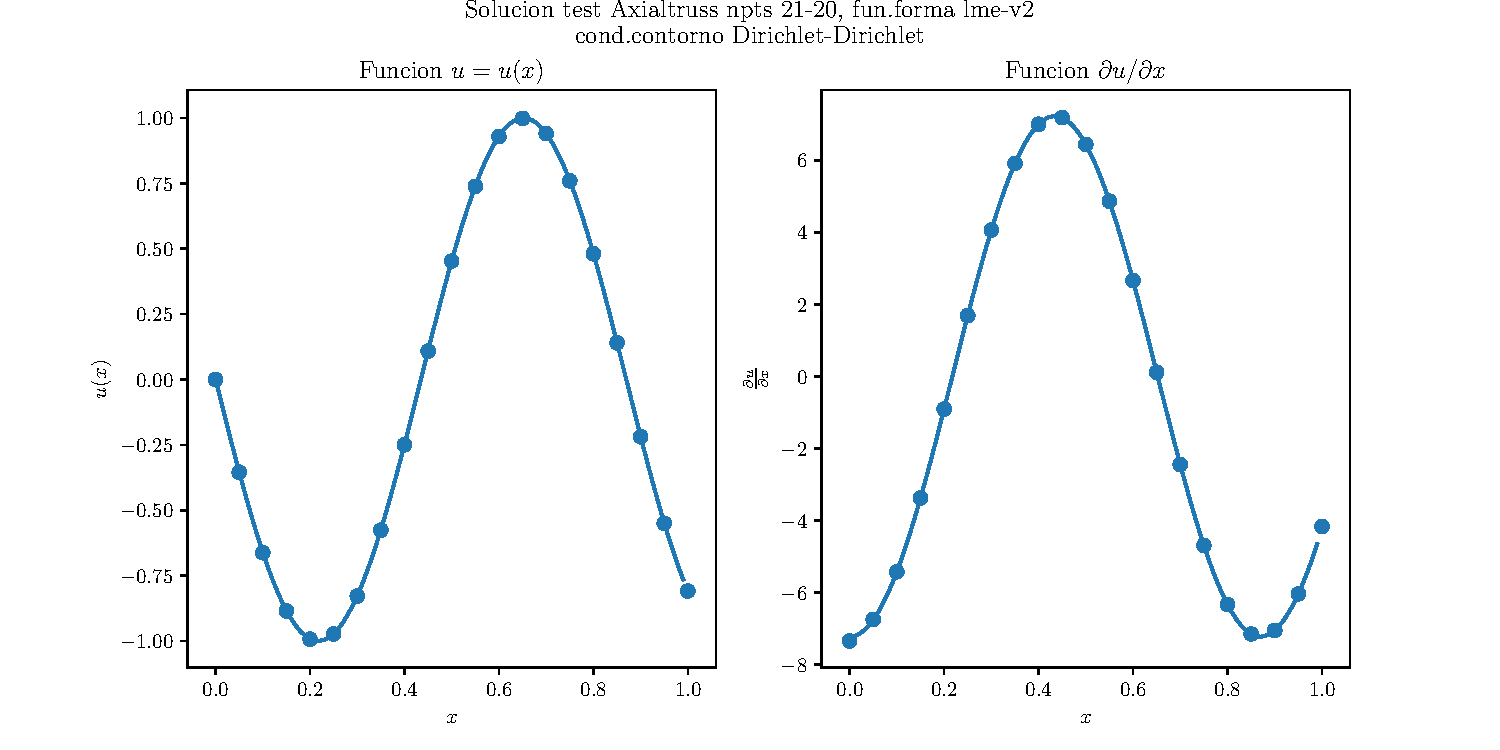
\includegraphics[width=1\textwidth]{./Imagenes/06/solucion/Axialtruss_21-20_regular_type-2_caso-1_lme-v2_direct_dgesv-lapack-blas.pdf}
    \caption{Solución del test Axialtruss} \label{fig:Axialtruss_caso-1_sol}
\end{figure}
%%%%%%%%%%%%%%%%%%%%%%%%%%%%%%%%%%%%%%%%%
\begin{figure}
    \centering
    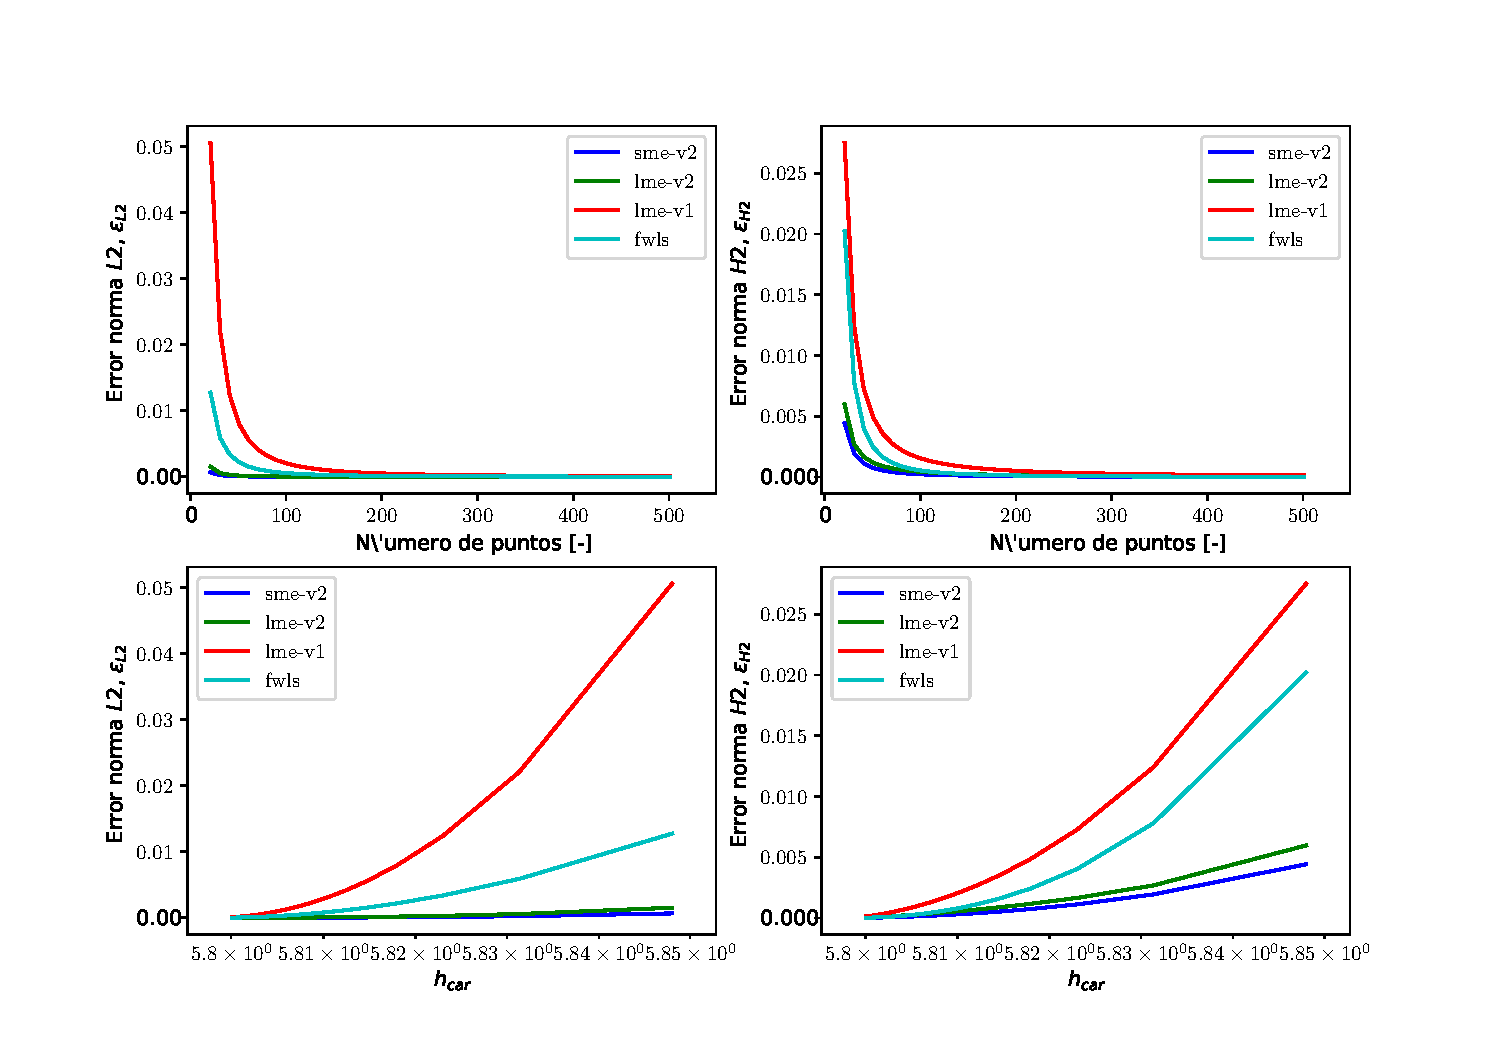
\includegraphics[width=1\textwidth]{./Imagenes/06/comparacion_shp_regular/Axialtruss_regular_type-2_caso-1_direct_dgesv-lapack-blas_sme-v2_lme-v2_lme-v1_fwls.pdf}
    \caption{Convergencia test Axialtruss sujeto a condiciones Dirichlet - Dirichlet para una distribución regular} \label{fig:Axialtruss_caso-1_conv}
\end{figure}
\begin{figure}
    \centering
    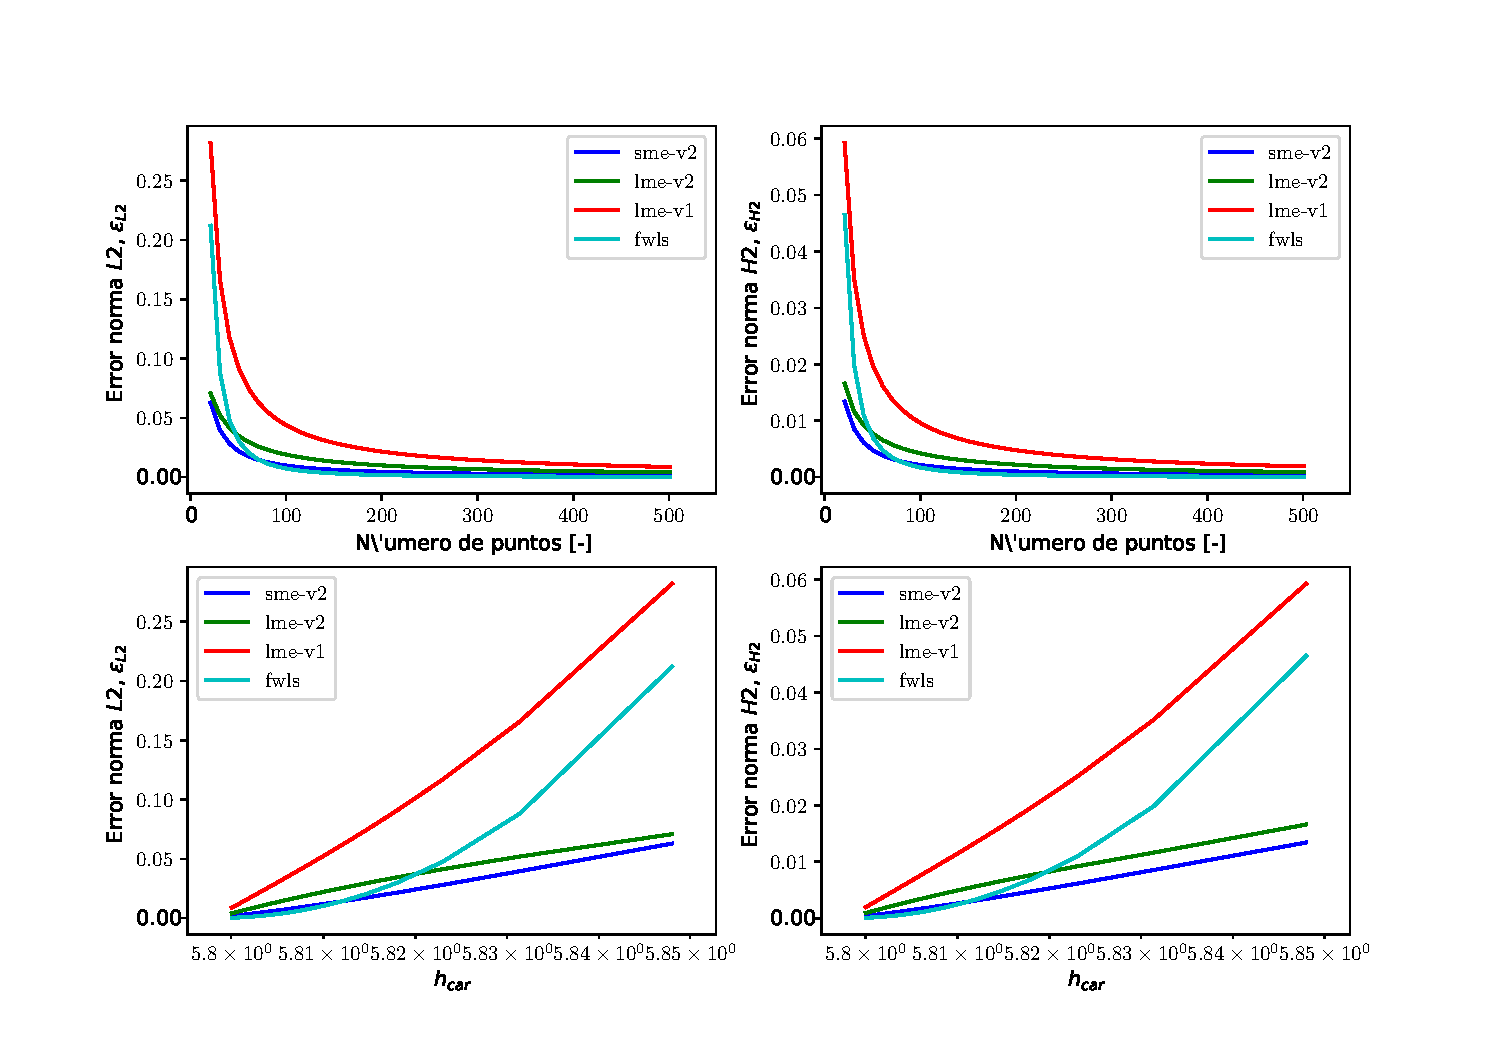
\includegraphics[width=1\textwidth]{./Imagenes/06/comparacion_shp_regular/Axialtruss_regular_type-2_caso-2_direct_dgesv-lapack-blas_sme-v2_lme-v2_lme-v1_fwls.pdf}
    \caption{Convergencia test Axialtruss sujeto a condiciones Neumann - Dirichlet para una distribución regular} \label{fig:Axialtruss_caso-2_conv}
\end{figure}
\begin{figure}
    \centering
    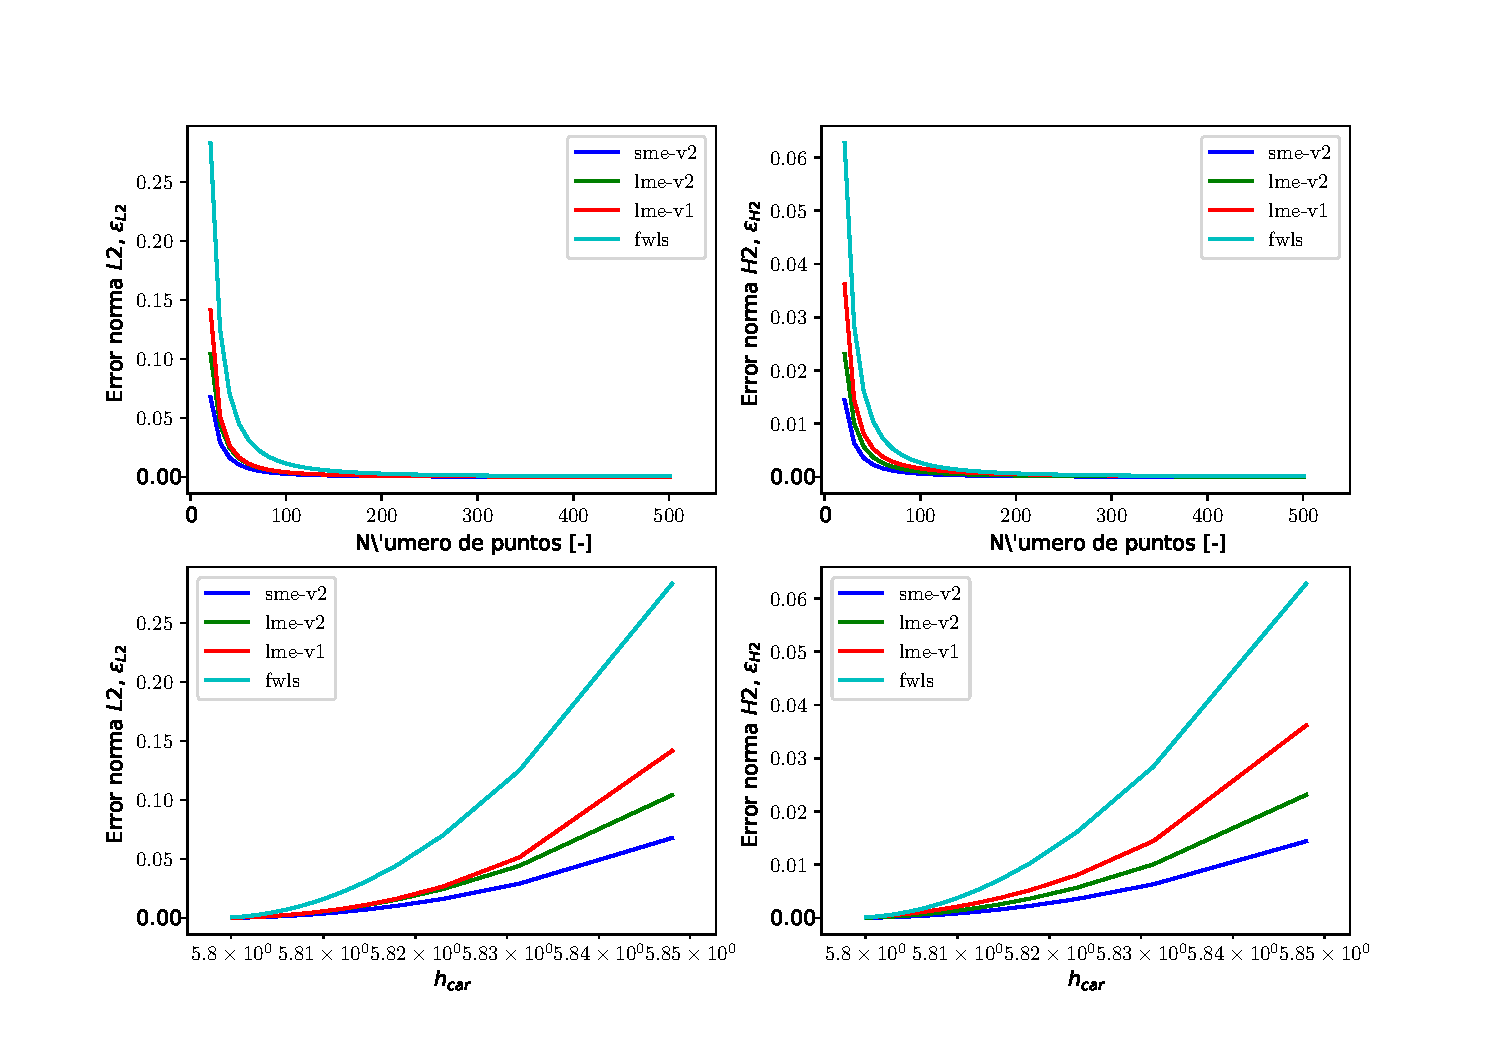
\includegraphics[width=1\textwidth]{./Imagenes/06/comparacion_shp_regular/Axialtruss_regular_type-2_caso-3_direct_dgesv-lapack-blas_sme-v2_lme-v2_lme-v1_fwls.pdf}
    \caption{Convergencia test Axialtruss sujeto a condiciones Dirichlet - Neumann para una distribución regular} \label{fig:Axialtruss_caso-3_conv}
\end{figure}
%%%%%%%%%%%%%%%%%%%%%%%%%%%%%%%%%%%%%%%%%
\begin{figure}
    \centering
    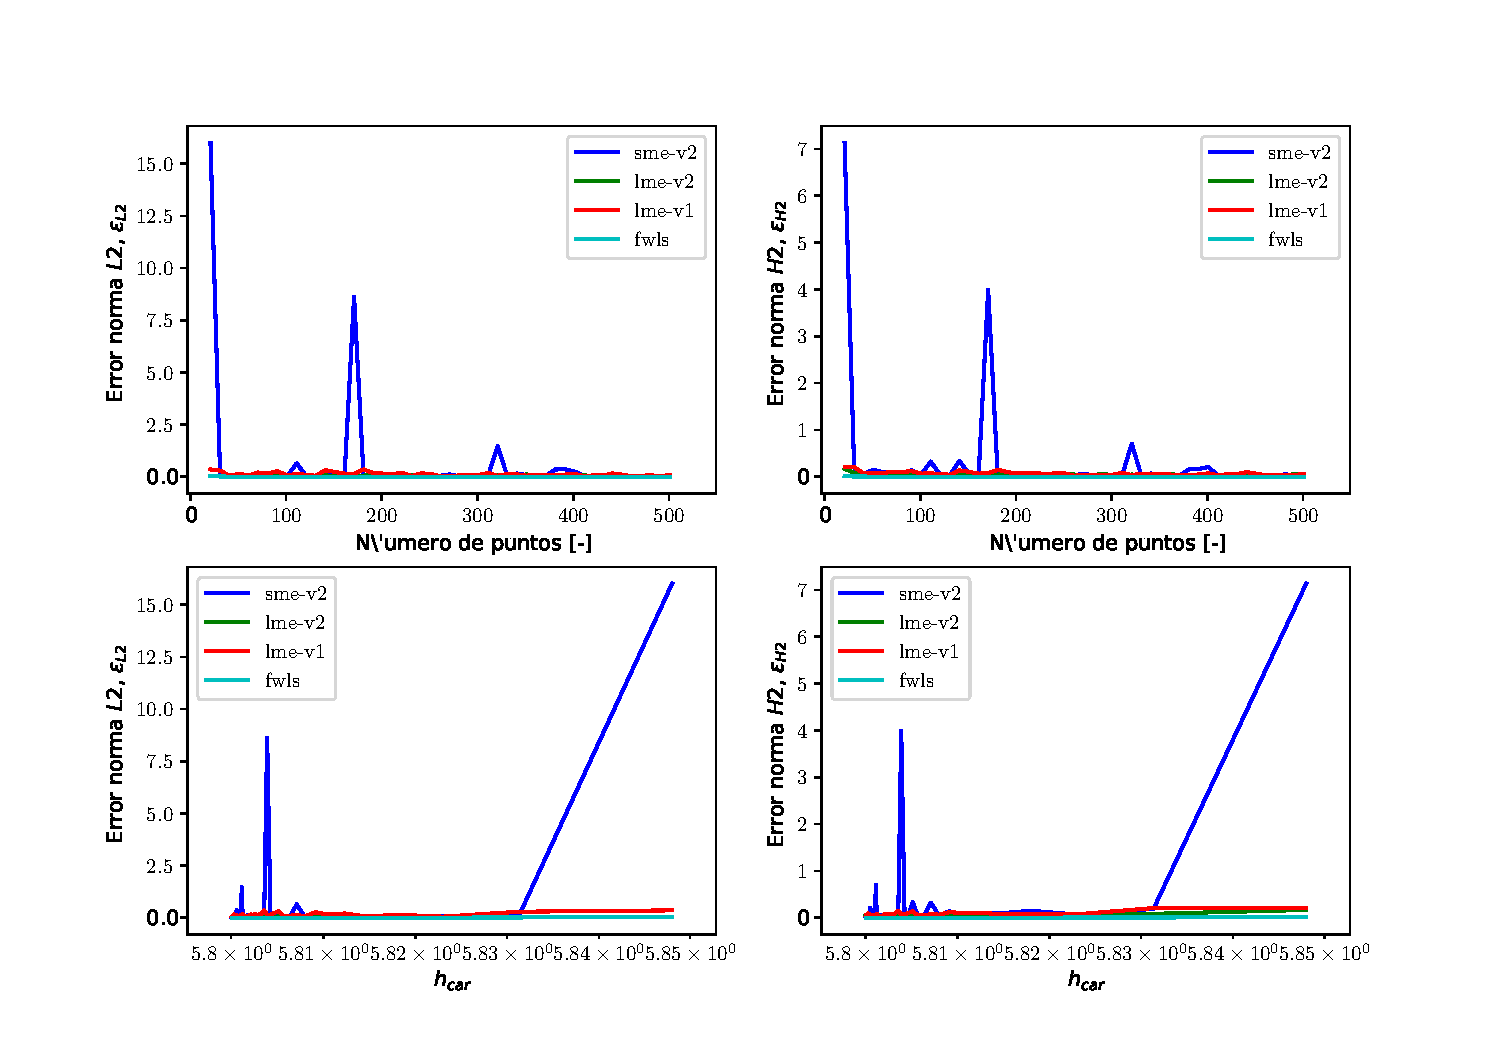
\includegraphics[width=1\textwidth]{./Imagenes/06/comparacion_shp_irreg/Axialtruss_irreg_type-2_caso-1_direct_dgesv-lapack-blas_sme-v2_lme-v2_lme-v1_fwls.pdf}
    \caption{Convergencia test Axialtruss sujeto a condiciones Dirichlet - Dirichlet para una distribución irregular} \label{fig:Axialtruss_caso-1_conv_irreg}
\end{figure}
\begin{figure}
    \centering
    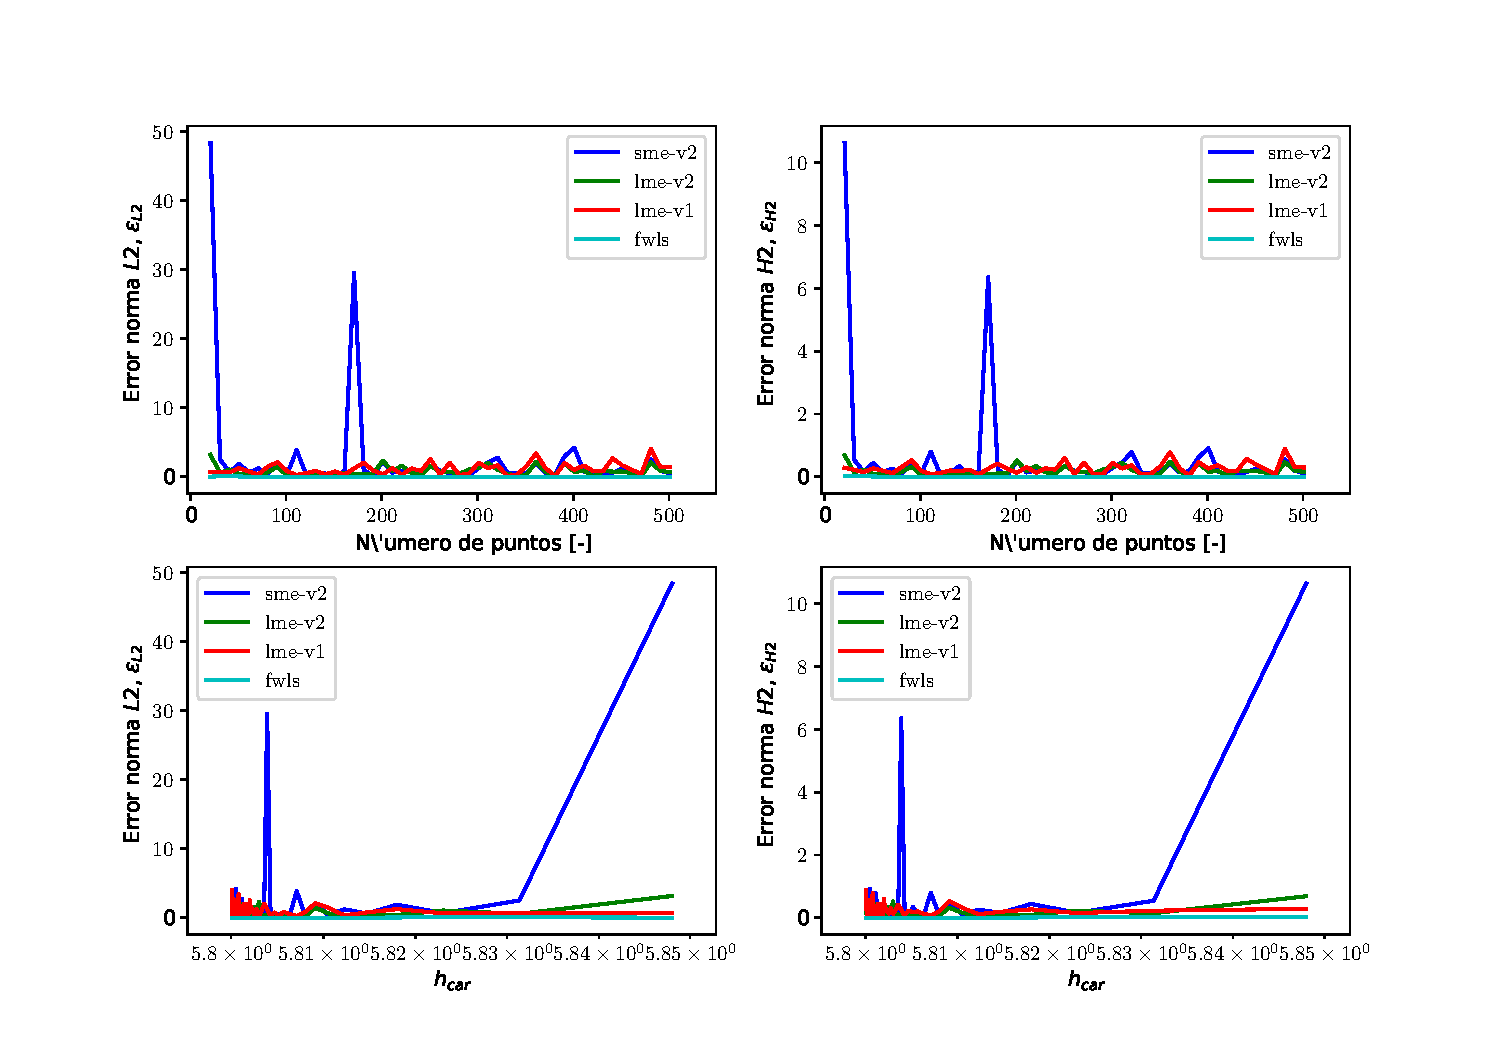
\includegraphics[width=1\textwidth]{./Imagenes/06/comparacion_shp_irreg/Axialtruss_irreg_type-2_caso-2_direct_dgesv-lapack-blas_sme-v2_lme-v2_lme-v1_fwls.pdf}
    \caption{Convergencia test Axialtruss sujeto a condiciones Neumann - Dirichlet para una distribución irregular} \label{fig:Axialtruss_caso-2_conv_irreg}
\end{figure}
\begin{figure}
    \centering
    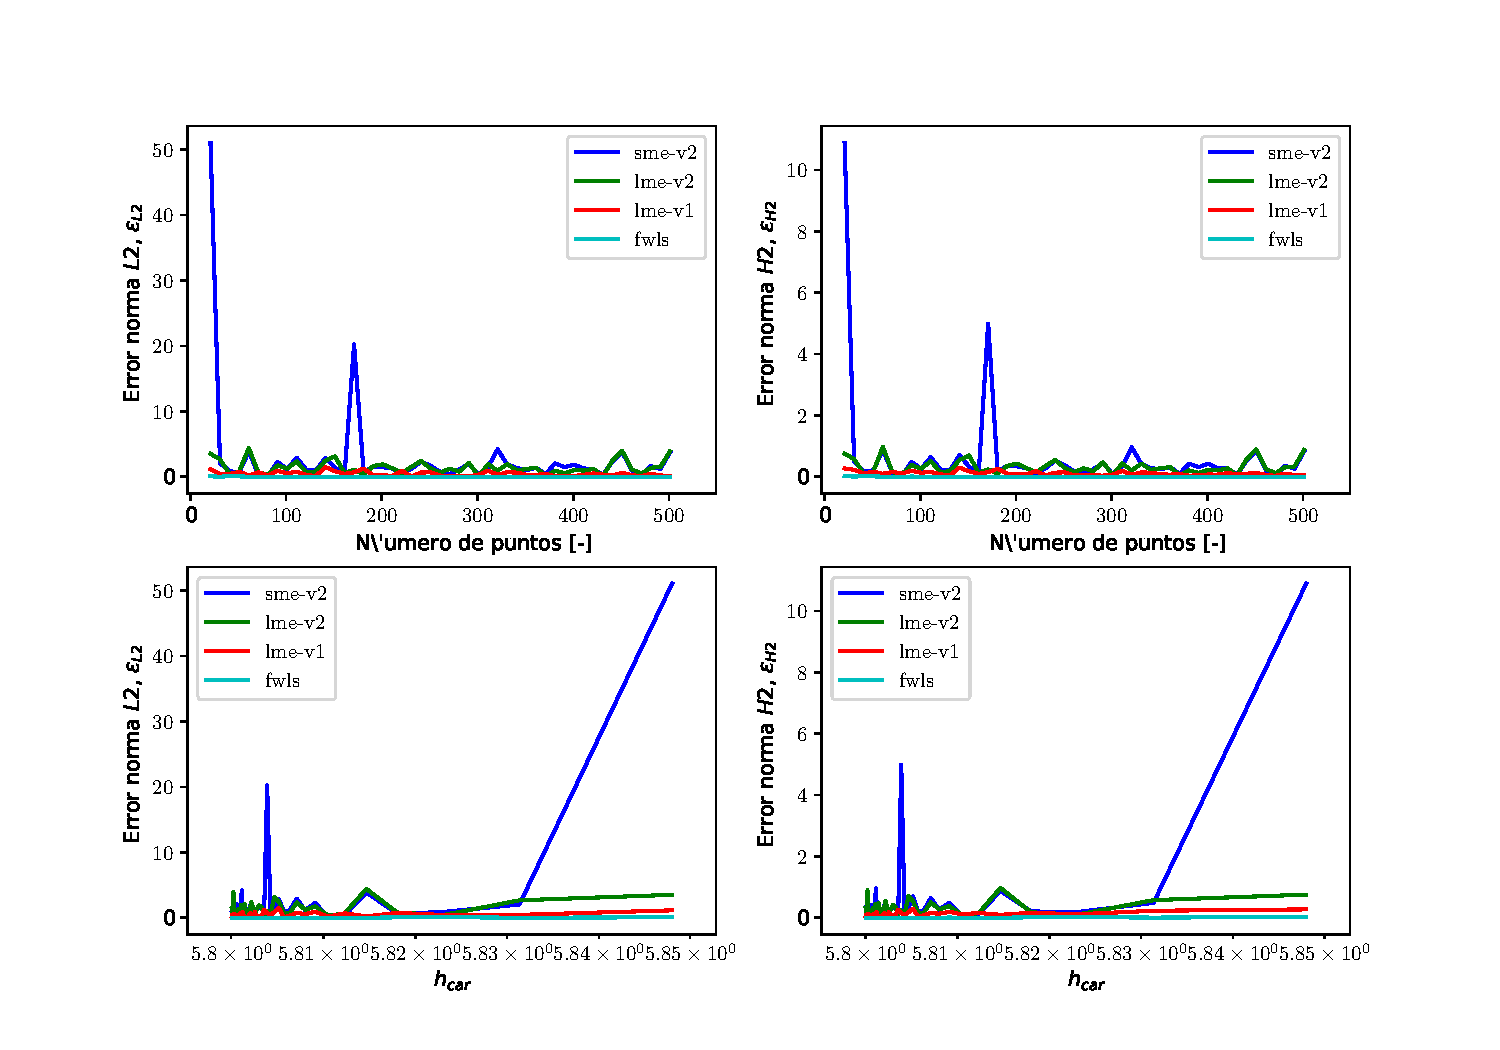
\includegraphics[width=1\textwidth]{./Imagenes/06/comparacion_shp_irreg/Axialtruss_irreg_type-2_caso-3_direct_dgesv-lapack-blas_sme-v2_lme-v2_lme-v1_fwls.pdf}
    \caption{Convergencia test Axialtruss sujeto a condiciones Dirichlet - Neumann para una distribución irregular} \label{fig:Axialtruss_caso-3_conv_irreg}
\end{figure}

%%%%%%%%%%%%%%%%%%%%%%%%%%%%%%%%%%%%%%%%%%%%%%%%%%%%%%%%%%%%%%%%%%%%

\subsection{Waveprop}
Se resuelve una ecuación unidimensional de onda de la forma:
\begin{equation}
    \frac{d^2u}{dx^2} + \lambda u = 0
\end{equation}
sujeto a las siguientes condiciones,
\begin{equation}
    u|_{x=0} \; , \; u|_{x=1} = 1
\end{equation}
se tiene la solución exacta,
\begin{eqnarray}
    u = \frac{ sin( \sqrt{\lambda} x) }{ sin( \sqrt{\lambda} ) }
    du = \sqrt{\lambda} \frac{ cos( \sqrt{\lambda} x )} {( sin( \sqrt{\lambda} ))}
\end{eqnarray}
En la Figura \ref{fig:Waveprop_caso-1_sol} se muestra la solución y en las Figuras \ref{fig:Waveprop_caso-1_conv} \ref{fig:Waveprop_caso-2_conv} \ref{fig:Waveprop_caso-3_conv} se muestra la convergencia de la solución
\begin{figure}
    \centering
    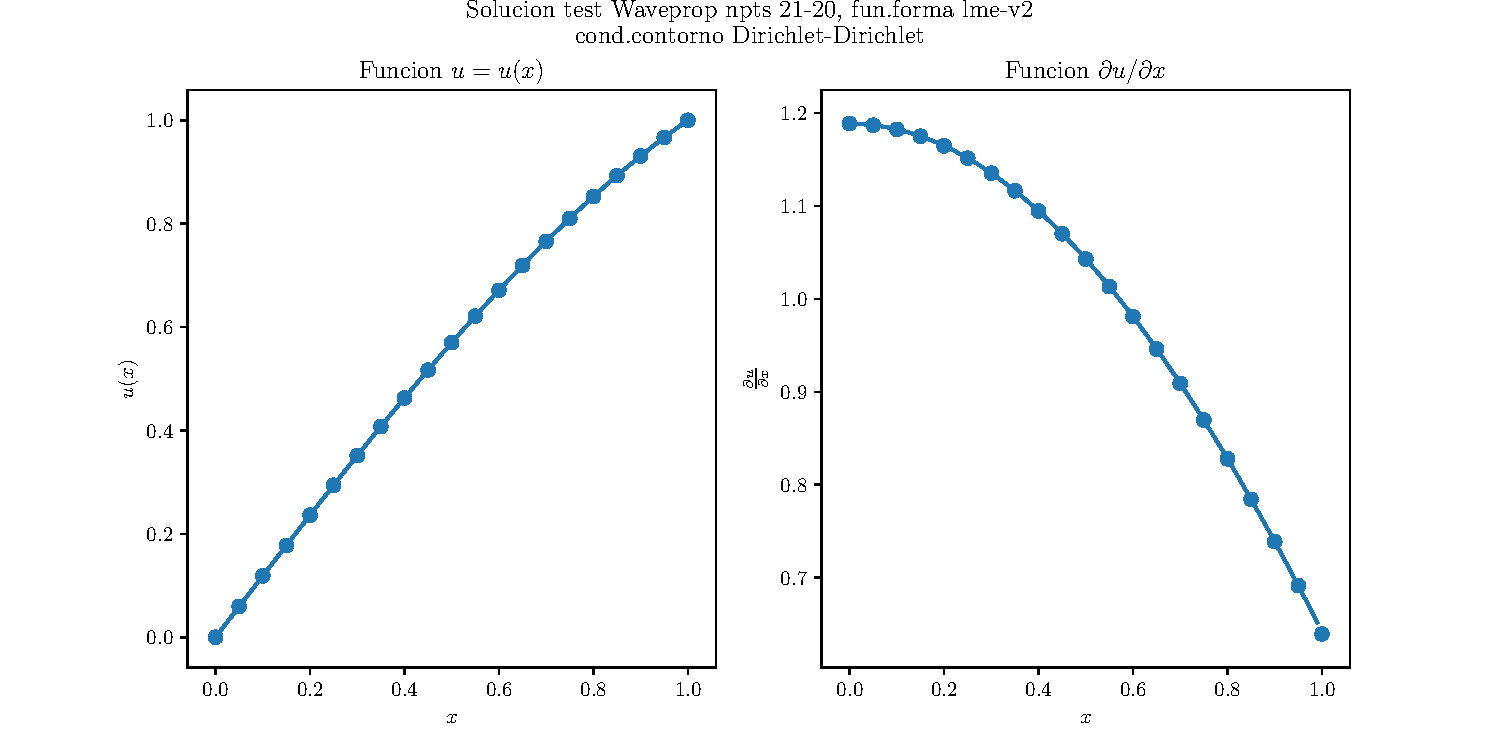
\includegraphics[width=1\textwidth]{./Imagenes/06/solucion/Waveprop_21-20_regular_type-2_caso-1_lme-v2_direct_dgesv-lapack-blas.pdf}
    \caption{Solución del test Waveprop} \label{fig:Waveprop_caso-1_sol}
\end{figure}
%%%%%%%%%%%%%%%%%%%%%%%%%%%%%%%%%%%%%%%%%
\begin{figure}
    \centering
    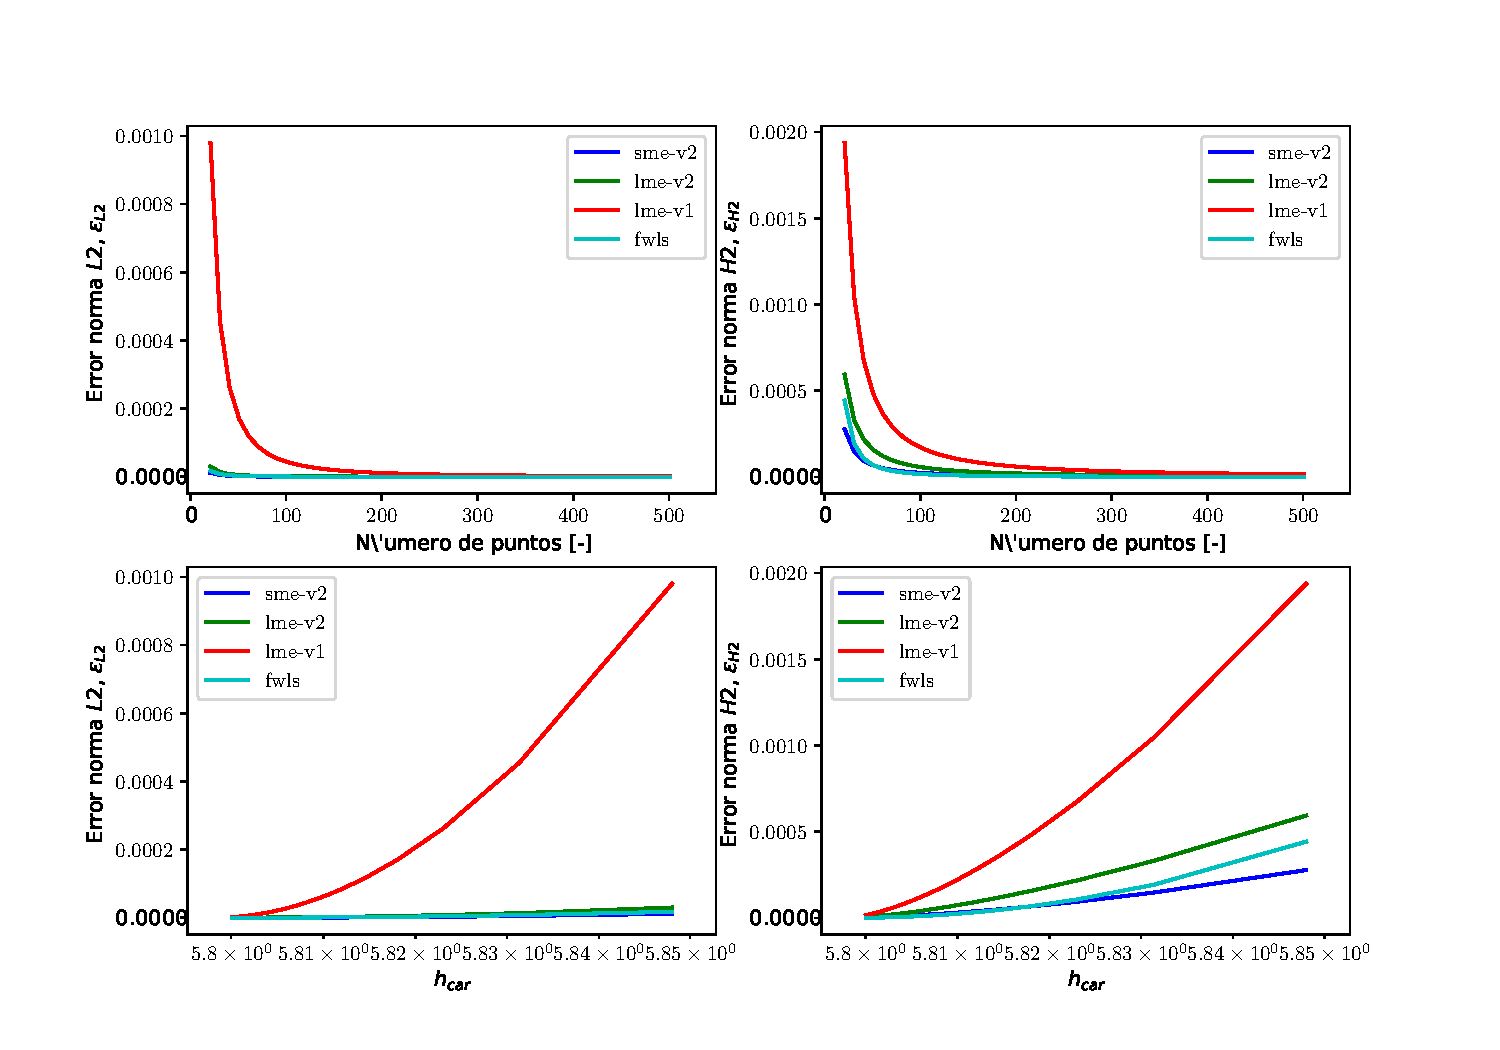
\includegraphics[width=1\textwidth]{./Imagenes/06/comparacion_shp_regular/Waveprop_regular_type-2_caso-1_direct_dgesv-lapack-blas_sme-v2_lme-v2_lme-v1_fwls.pdf}
    \caption{Convergencia test Waveprop sujeto a condiciones Dirichlet - Dirichlet para una distribución regular} \label{fig:Waveprop_caso-1_conv}
\end{figure}
\begin{figure}
    \centering
    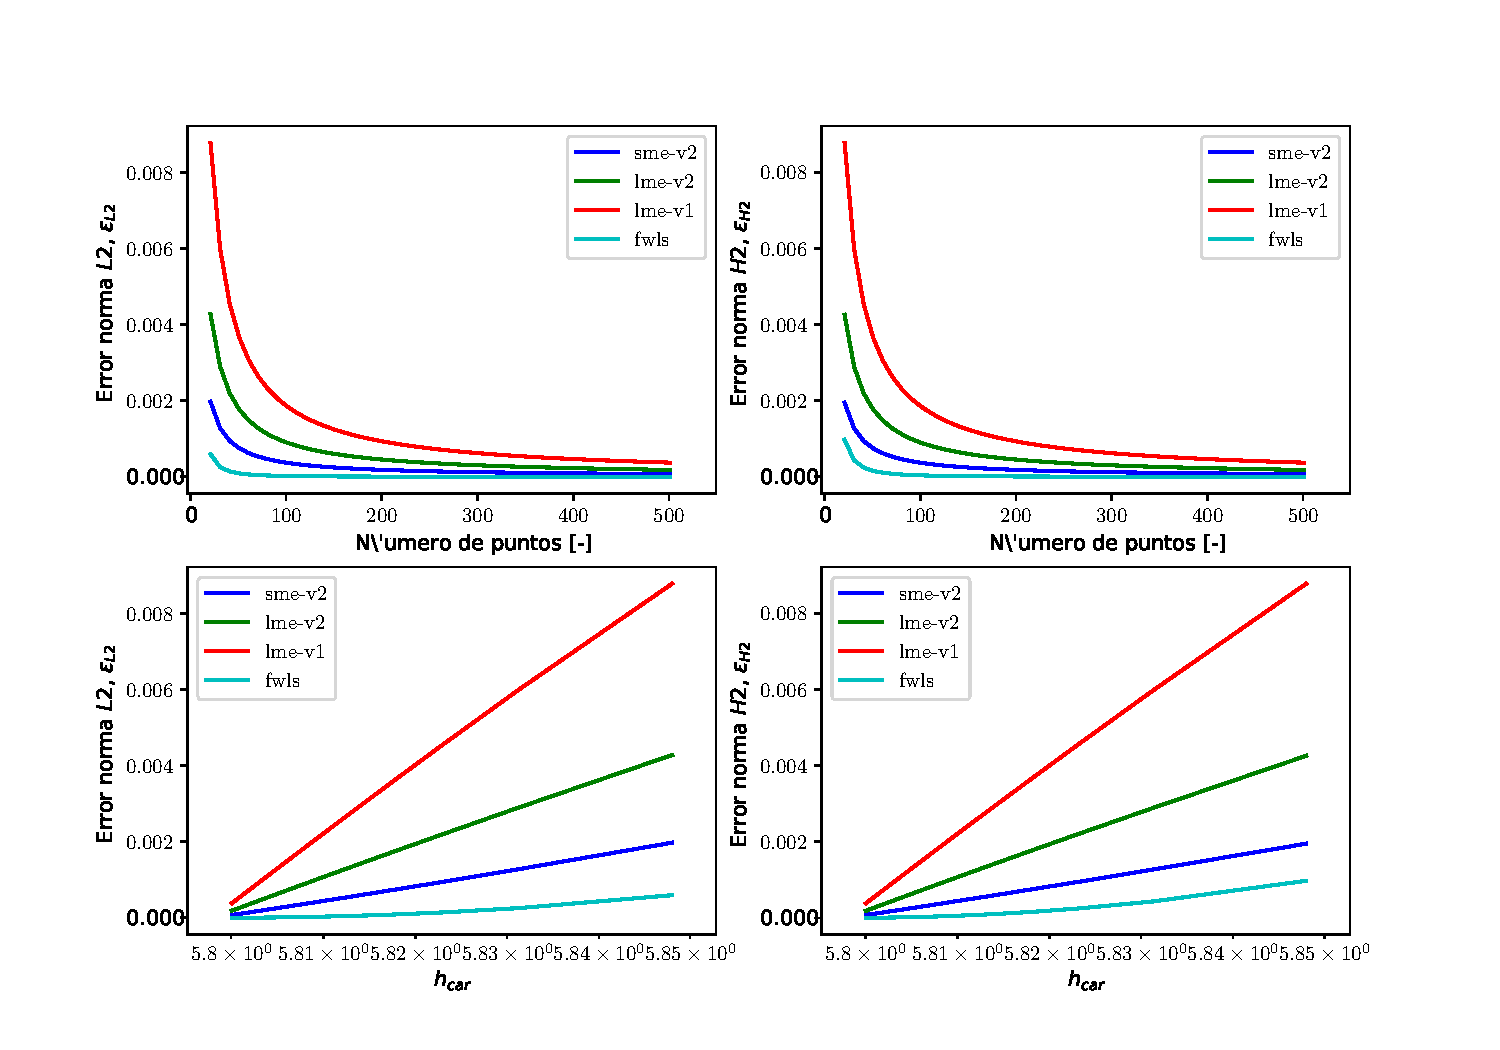
\includegraphics[width=1\textwidth]{./Imagenes/06/comparacion_shp_regular/Waveprop_regular_type-2_caso-2_direct_dgesv-lapack-blas_sme-v2_lme-v2_lme-v1_fwls.pdf}
    \caption{Convergencia test Waveprop sujeto a condiciones Dirichlet - Neumann para una distribución regular} \label{fig:Waveprop_caso-2_conv}
\end{figure}
\begin{figure}
    \centering
    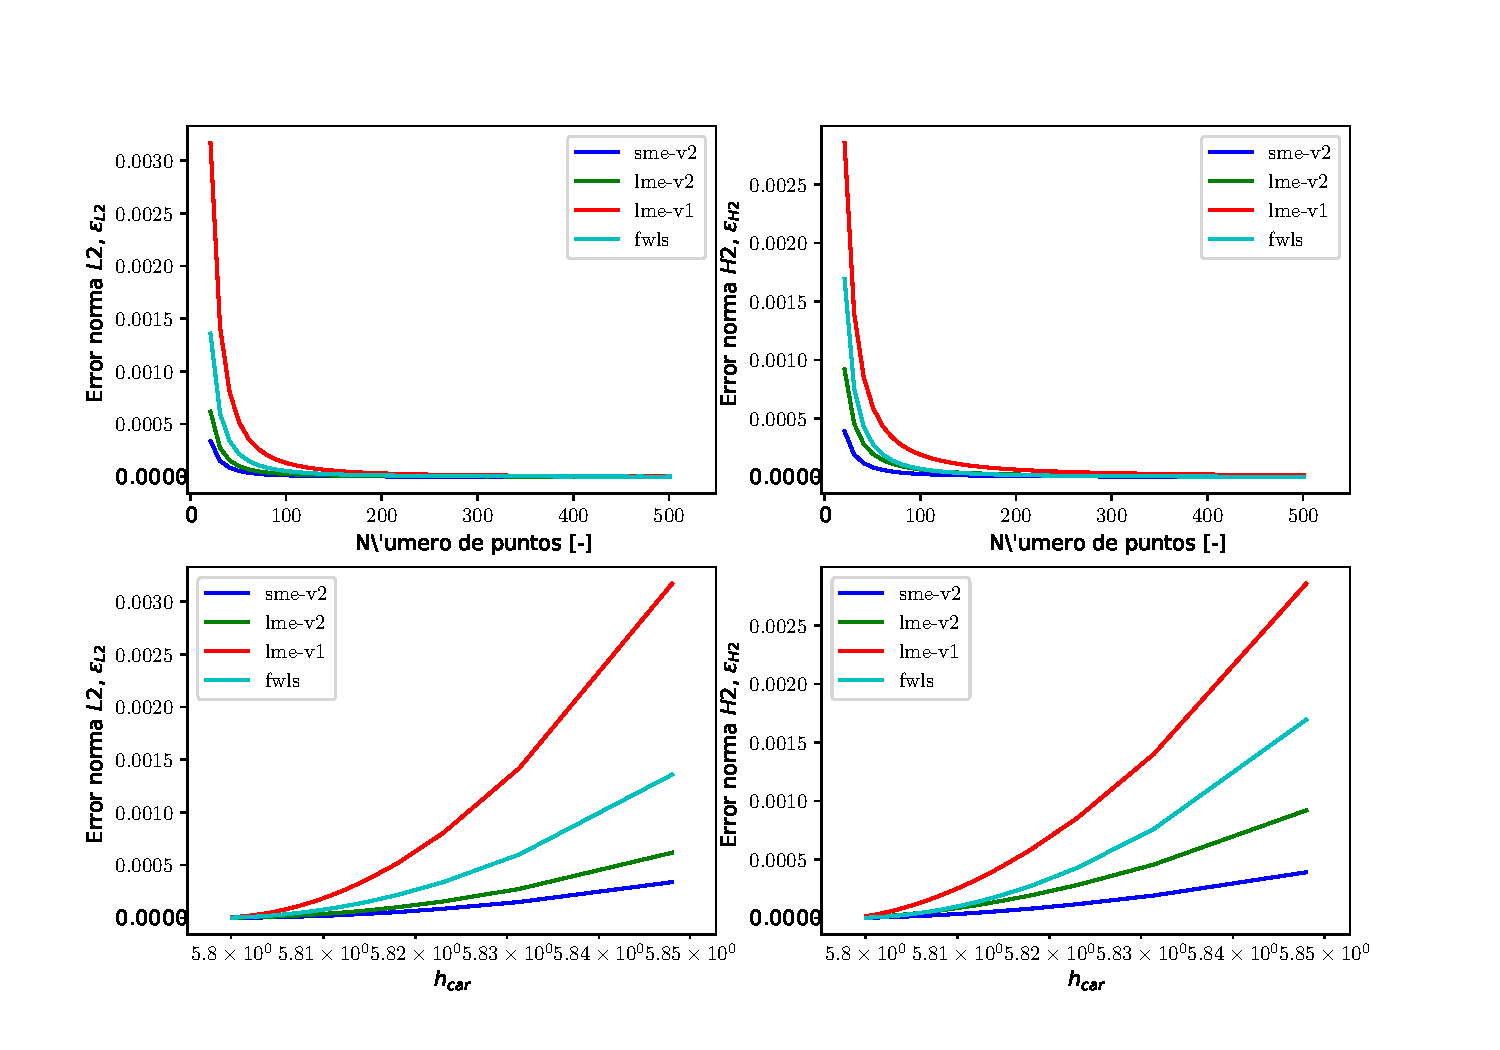
\includegraphics[width=1\textwidth]{./Imagenes/06/comparacion_shp_regular/Waveprop_regular_type-2_caso-3_direct_dgesv-lapack-blas_sme-v2_lme-v2_lme-v1_fwls.pdf}
    \caption{Convergencia test Waveprop sujeto a condiciones Neumann - Dirichlet para una distribución regular} \label{fig:Waveprop_caso-3_conv}
\end{figure}
%%%%%%%%%%%%%%%%%%%%%%%%%%%%%%%%%%%%%%%%%
\begin{figure}
    \centering
    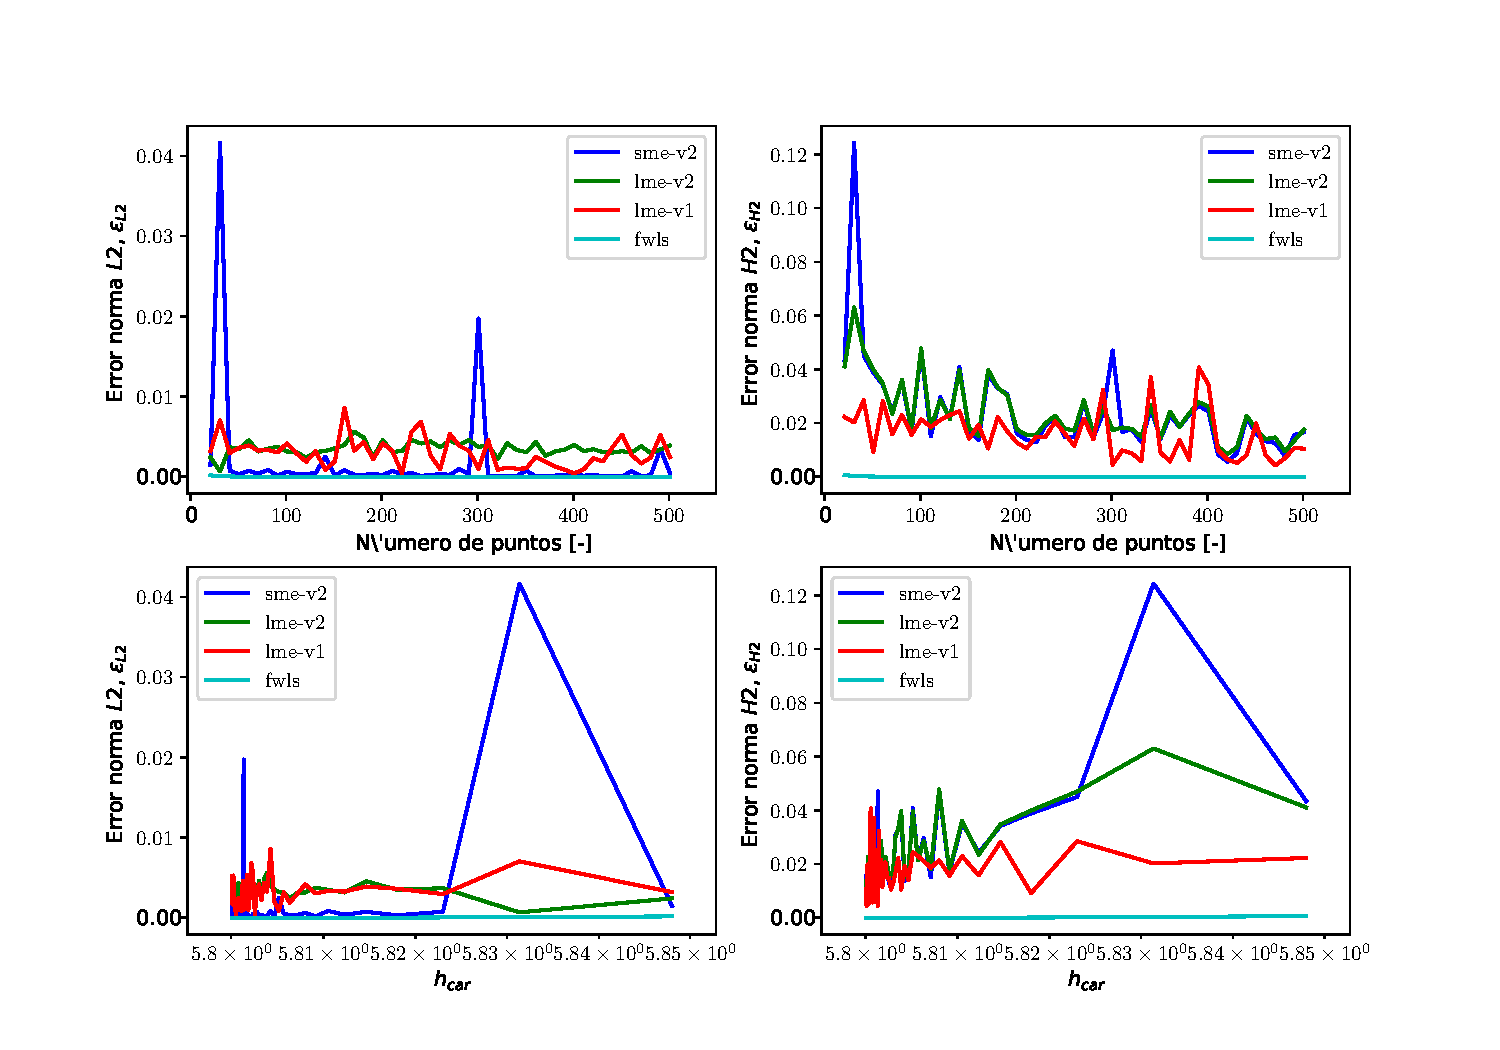
\includegraphics[width=1\textwidth]{./Imagenes/06/comparacion_shp_irreg/Waveprop_irreg_type-2_caso-1_direct_dgesv-lapack-blas_sme-v2_lme-v2_lme-v1_fwls.pdf}
    \caption{Convergencia test Waveprop sujeto a condiciones Dirichlet - Dirichlet para una distribución irregular} \label{fig:Waveprop_caso-1_conv_irreg}
\end{figure}
\begin{figure}
    \centering
    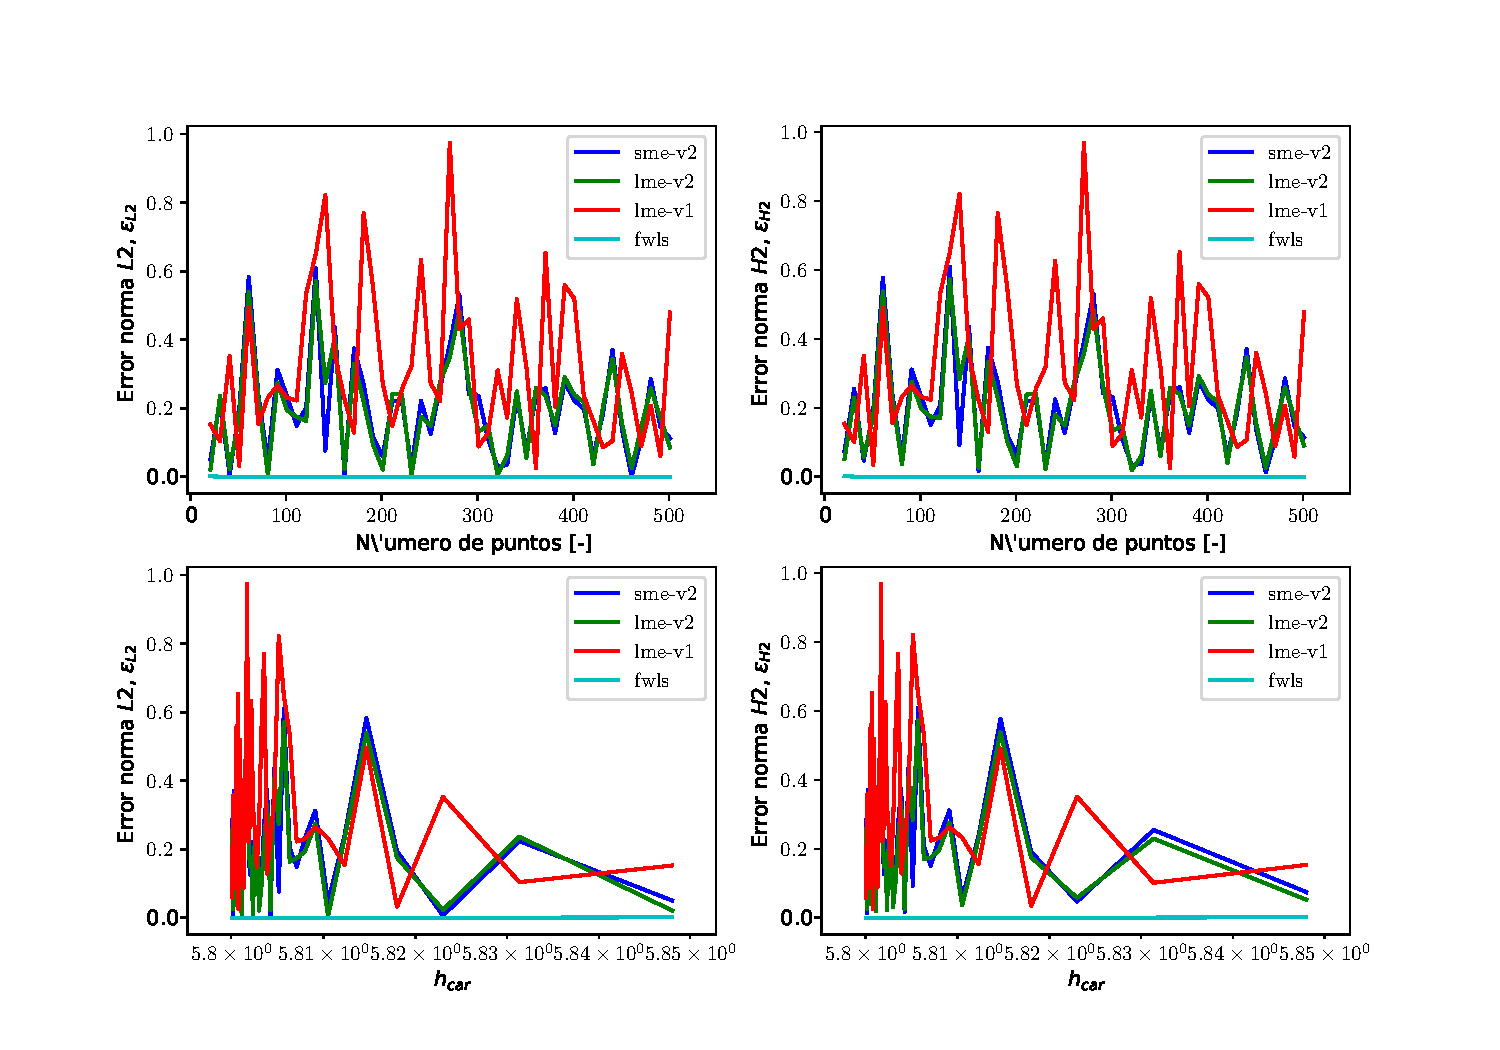
\includegraphics[width=1\textwidth]{./Imagenes/06/comparacion_shp_irreg/Waveprop_irreg_type-2_caso-2_direct_dgesv-lapack-blas_sme-v2_lme-v2_lme-v1_fwls.pdf}
    \caption{Convergencia test Waveprop sujeto a condiciones Dirichlet - Neumann para una distribución irregular} \label{fig:Waveprop_caso-2_conv_irreg}
\end{figure}
\begin{figure}
    \centering
    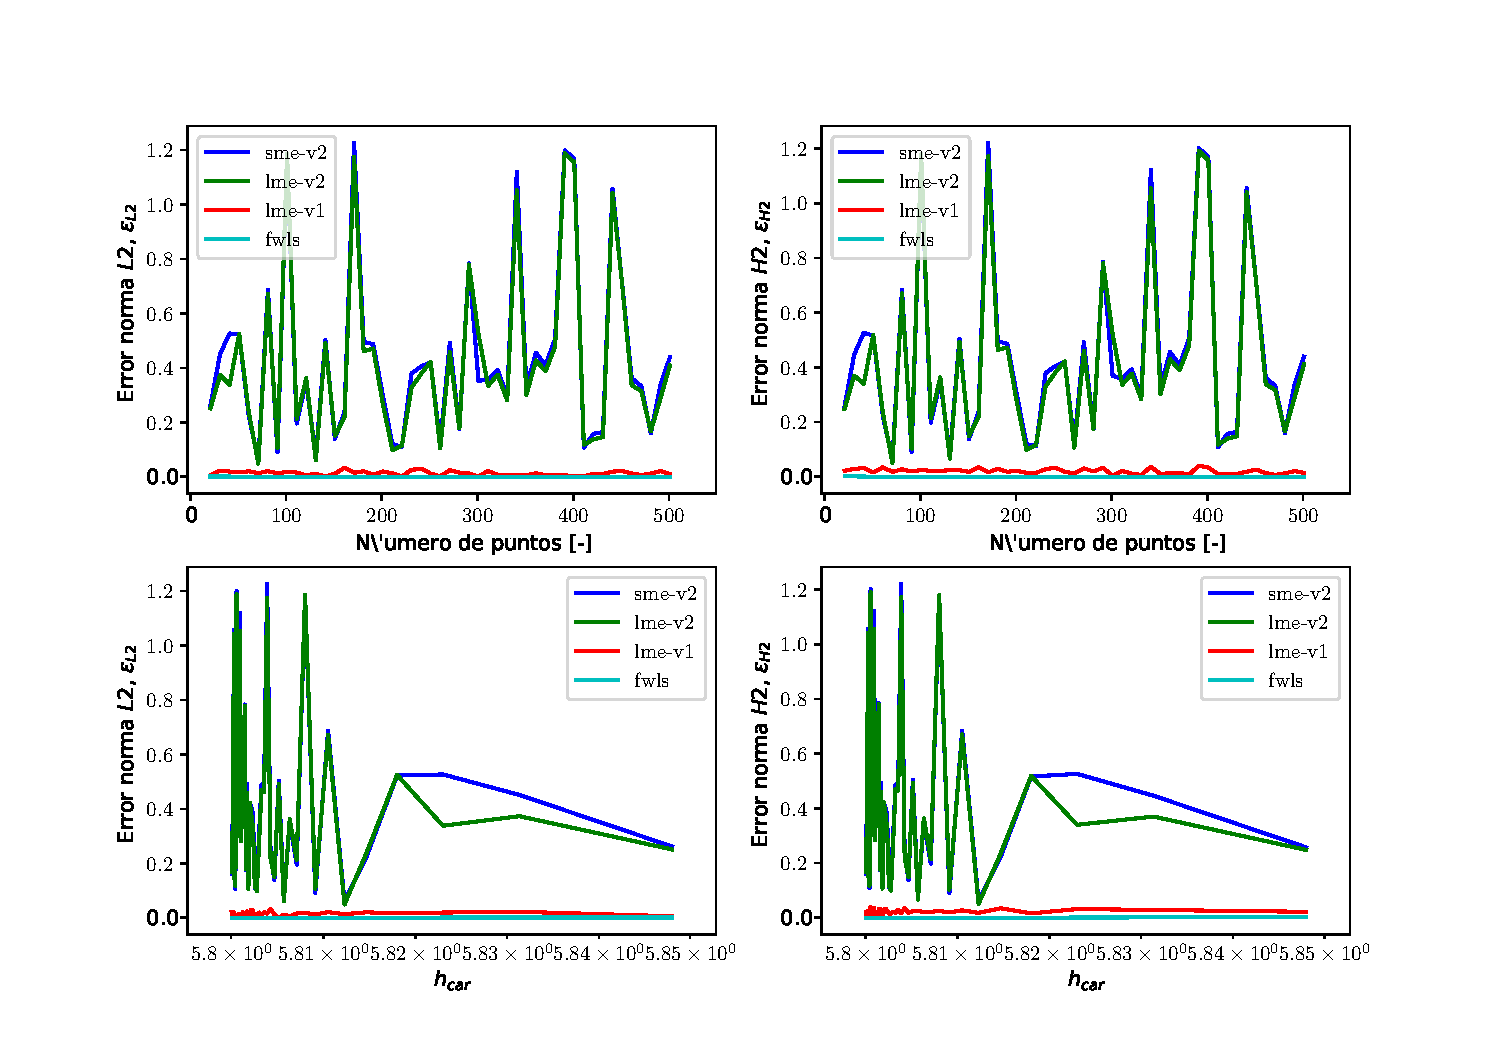
\includegraphics[width=1\textwidth]{./Imagenes/06/comparacion_shp_irreg/Waveprop_irreg_type-2_caso-3_direct_dgesv-lapack-blas_sme-v2_lme-v2_lme-v1_fwls.pdf}
    \caption{Convergencia test Waveprop sujeto a condiciones Neumann - Dirichlet para una distribución irregular} \label{fig:Waveprop_caso-3_conv_irreg}
\end{figure}


